\chapter{Implementation}
\label{chap:implementation}


\section{Architecture}
\setlength{\leftskip}{0.25cm}
\indent \indent
This section is dedicated to detailing the high-level architecture and design of the project. It will discuss the purpose of each component and the software engineering principles applied to make design choices.

\setlength{\leftskip}{0cm}
\subsection{Framework}
\setlength{\leftskip}{0.5cm}
\indent \indent
The project's design began with understanding the MLaaS threat model described in §\ref{sec:threatModel}. Figure \ref{fig:abstractNetwork} depicts a high-level layout of the core components based on this framework. The server-side application has been split into two categories: \textit{online} in red and \textit{offline} in blue. Online describes inference being performed directly in response to a request from the client. Offline describes generating inference results on batches of data, independent of the front-end. 
\begin{itemize}
    \item The online components are where most of this dissertation's discussion occurs. This portion of the application is responsible for emulating the MLaaS model. The \textit{GUI} allows users to select the encryption scheme and inference method used. The user's video is then passed to the \textit{encryption} component, responsible for encrypting data using the selected scheme - either CKKS or MeKKS in the current implementation. The resulting encrypted data is then passed through the \textit{client} to the \textit{server}. In the \textit{inference} component, the received data is privately analysed, and a video containing only the moving objects is returned to the \textit{client} via the \textit{server}. The \textit{decryption} component must then decrypt the inference results and the video played for the user.
    \item The offline components are intended for use before the application is deployed. The framework's \textit{testing} component refers to developing and refining the inference algorithms used to extract moving objects. The \textit{evaluation} component encompasses the process of evaluating the application, including both inference performance and client-server activity.
\end{itemize}
\indent \indent
Figure \ref{fig:abstractInference} provides a deeper insight into the composition of the inference component. The scope of this project only considers the layers above encryption primitives. However, it is important to note that lower layers of abstraction exist. In particular, a layer that may be particularly relevant to the investigation begun by this dissertation is the hardware implementation. Hardware modifications could potentially impact the application's performance considerably, both positively and negatively. For example, accelerators, such as GPUs, could be used to perform cryptographic operations ~\cite{Badawi}. Equally, the hardware used in current surveillance implementations may produce weaker results.
\begin{figure}[ht]
    \begin{subfigure}[b]{0.5\textwidth}
        \centering
        \scalebox{0.5}{\begin{tikzpicture}
    \draw[draw=black,dashed,line width=0.5mm] (0,-3) rectangle ++(12,10);
    \node (Encryption) at (3,2) [draw,thick,minimum width=4cm,minimum height=2cm,fill=ckksRed] {\Large\textrm{Encryption}};
    \node (Decryption) at (9,2) [draw,thick,minimum width=4cm,minimum height=2cm,fill=ckksRed] {\Large\textrm{Decryption}};
    \node (GUI) at (6,-1) [draw,thick,minimum width=7cm,minimum height=2cm,fill=ckksRed] {\Large\textrm{Graphical User Interface}};
    \node (Client) at (6,5) [draw,thick,minimum width=7cm,minimum height=2cm,fill=ckksRed] {\Large\textrm{Client}};

    \draw[->,>=stealth,line width=1mm] ([xshift=-2cm]GUI.north) to ([xshift=1cm]Encryption.south);
    \draw[->,>=stealth,line width=1mm] ([xshift=-1cm]Decryption.south) to ([xshift=2cm]GUI.north);
    \draw[->,>=stealth,line width=1mm] ([xshift=1cm]Encryption.north) to ([xshift=-2cm]Client.south);
    \draw[->,>=stealth,line width=1mm] ([xshift=2cm]Client.south) to ([xshift=-1cm]Decryption.north);



    \draw[draw=black,dashed,line width=0.5mm] (0,10) rectangle ++(12,10);
    \node (Server) at (6,12) [draw,thick,minimum width=7cm,minimum height=2cm,fill=ckksRed] {\Large\textrm{Server}};
    \node (Inference) at (6,15) [draw,thick,minimum width=7cm,minimum height=2cm,fill=ckksRed] {\Large\textrm{Inference}};
    \node (Testing) at (9,18) [draw,thick,minimum width=4cm,minimum height=2cm,fill=mekksBlue] {\Large\textrm{Testing}};
    \node (Evaluation) at (3,18) [draw,thick,minimum width=4cm,minimum height=2cm,fill=mekksBlue] {\Large\textrm{Evaluation}};

    \draw[->,>=stealth,line width=1mm] ([xshift=-2cm]Server.north) to ([xshift=-2cm]Inference.south);
    \draw[->,>=stealth,line width=1mm] ([xshift=2cm]Inference.south) to ([xshift=2cm]Server.north);



    \draw[->,>=stealth,line width=1mm] ([xshift=-2cm]Client.north) to ([xshift=-2cm]Server.south);
    \draw[->,>=stealth,line width=1mm] ([xshift=2cm]Server.south) to ([xshift=2cm]Client.north);
\end{tikzpicture}
}
        \captionsetup{justification=centering}
        \caption[Project Components]{The project components.\medskip\\Online:\sethlcolor{ckksRed} \hl{\quad\quad\quad\quad}\smallskip\\Offline:\sethlcolor{mekksBlue} \hl{\quad\quad\quad\quad}}
        \label{fig:abstractNetwork}
    \end{subfigure}%
    \begin{subfigure}[b]{0.5\textwidth}
        \centering
        \scalebox{0.7}{\begin{tikzpicture}
    \coordinate (Start) at (2.5,14);
    \coordinate (End) at (6.5,14);
    \coordinate (aStart) at (10,0);
    \coordinate (aEnd) at (10,13);


    \draw[draw=black,dashed,line width=0.5mm] (0,0) rectangle ++(9,13);
    \node (Inference) at (4.5,11) [draw,thick,minimum width=7cm,minimum height=2cm,fill=abstractYellow] {\Large\textrm{Inference}};
    \node (Arithmetic) at (4.5,8) [draw,thick,minimum width=7cm,minimum height=2cm,fill=abstractYellow] {\Large\textrm{Arithmetic}};
    \node (Circuits) at (4.5,5) [draw,thick,minimum width=7cm,minimum height=2cm,fill=abstractYellow] {\Large\textrm{Boolean Circuits}};
    \node (Primitives) at (4.5,2) [draw,thick,minimum width=7cm,minimum height=2cm,fill=abstractYellow] {\Large\textrm{Cryptographic Primitives}};


    \draw[->,>=stealth,line width=0.8mm] (Start) to ([xshift=-2cm]Inference.north);
    \draw[->,>=stealth,line width=0.8mm] ([xshift=-2cm]Inference.south) to ([xshift=-2cm]Arithmetic.north);
    \draw[->,>=stealth,line width=0.8mm] ([xshift=-2cm]Arithmetic.south) to ([xshift=-2cm]Circuits.north);
    \draw[->,>=stealth,line width=0.8mm] ([xshift=-2cm]Circuits.south) to ([xshift=-2cm]Primitives.north);
    \draw[->,>=stealth,line width=0.8mm] ([xshift=2cm]Primitives.north) to ([xshift=2cm]Circuits.south);
    \draw[->,>=stealth,line width=0.8mm] ([xshift=2cm]Circuits.north) to ([xshift=2cm]Arithmetic.south);
    \draw[->,>=stealth,line width=0.8mm] ([xshift=2cm]Arithmetic.north) to ([xshift=2cm]Inference.south);
    \draw[->,>=stealth,line width=0.8mm] ([xshift=2cm]Inference.north) to (End);
    
    \draw[->,>=stealth,line width=1.2mm] (aStart) to (aEnd) node[rotate=270,sloped,anchor=center,above,xshift=6.5cm] {\large\textrm{Level of Abstraction}};

    % \node (Encryption) at (3,2) [draw,thick,minimum width=4cm,minimum height=2cm,fill=ckksRed] {\Large\textrm{Encryption}};
    % \node (Decryption) at (9,2) [draw,thick,minimum width=4cm,minimum height=2cm,fill=ckksRed] {\Large\textrm{Decryption}};
    % \node (GUI) at (6,-1) [draw,thick,minimum width=7cm,minimum height=2cm,fill=ckksRed] {\Large\textrm{Graphical User Interface}};
    % \node (Client) at (6,5) [draw,thick,minimum width=7cm,minimum height=2cm,fill=ckksRed] {\Large\textrm{Client}};

    % \draw[->,>=stealth,line width=0.6mm] ([xshift=-1cm]Decryption.south) to ([xshift=2cm]GUI.north);
    % \draw[->,>=stealth,line width=0.6mm] ([xshift=1cm]Encryption.north) to ([xshift=-2cm]Client.south);
    % \draw[->,>=stealth,line width=0.6mm] ([xshift=2cm]Client.south) to ([xshift=-1cm]Decryption.north);



    % \draw[draw=black,dashed,line width=0.5mm] (0,10) rectangle ++(12,10);
    % \node (Server) at (6,12) [draw,thick,minimum width=7cm,minimum height=2cm,fill=ckksRed] {\Large\textrm{Server}};
    % \node (Inference) at (6,15) [draw,thick,minimum width=7cm,minimum height=2cm,fill=ckksRed] {\Large\textrm{Inference}};
    % \node (Testing) at (9,18) [draw,thick,minimum width=4cm,minimum height=2cm,fill=mekksBlue] {\Large\textrm{Testing}};
    % \node (Evaluation) at (3,18) [draw,thick,minimum width=4cm,minimum height=2cm,fill=mekksBlue] {\Large\textrm{Evaluation}};

    % \draw[->,>=stealth,line width=0.6mm] ([xshift=-2cm]Server.north) to ([xshift=-2cm]Inference.south);
    % \draw[->,>=stealth,line width=0.6mm] ([xshift=2cm]Inference.south) to ([xshift=2cm]Server.north);



    % \draw[->,>=stealth,line width=0.6mm] ([xshift=-2cm]Client.north) to ([xshift=-2cm]Server.south);
    % \draw[->,>=stealth,line width=0.6mm] ([xshift=2cm]Server.south) to ([xshift=2cm]Client.north);
\end{tikzpicture}
}
        \caption{Abstract layers of the inference stack.}
        \label{fig:abstractInference}
    \end{subfigure}%
    \caption{High-level implementation overview.}
    \label{fig:abstraction}
\end{figure}

\setlength{\leftskip}{0cm}
\subsection{Software Interface}
\setlength{\leftskip}{0.5cm}
\indent \indent
An overview of the project's repository is given in Figure \ref{fig:filetree}. The project was written to clearly distinguish the layers depicted in Figure \ref{fig:abstraction}. The object-oriented approach to design allowed separate components to be implemented independently. As well as aiding comprehension, this architecture was chosen to minimise interaction across abstraction layers, and make the project straightforward to expand with, for example, more HE schemes or inference methods.
\smallskip \\ \indent
The application can be split into four layers of abstraction, from the high-level interface to the low-level implementation.
\begin{itemize}
    \item The highest level is the graphical user interface that the user directly interacts with. It allows the user to configure the encryption scheme and inference method used by the server, and upload and receive videos.
    \item The next layer contains the networking functionality of the application. Managed by the \texttt{connection} files in both the \texttt{client} and \texttt{server} packages, this layer is responsible for passing any data between the client and the server.
    \item The third layer establishes the API for the cryptographic principles. The HE functionality required by the application is contained within this layer so that the particular scheme in use can be substituted without changes to the above layers.
    \item The lowest level contains the cryptographic primitives. Contained within the \texttt{lib} folder, the libraries \texttt{Seal-Python} and \texttt{MeKKS} contain the implementations of these primitives so that the preceding levels may use them.
\end{itemize}

\begin{figure}[htp]     
    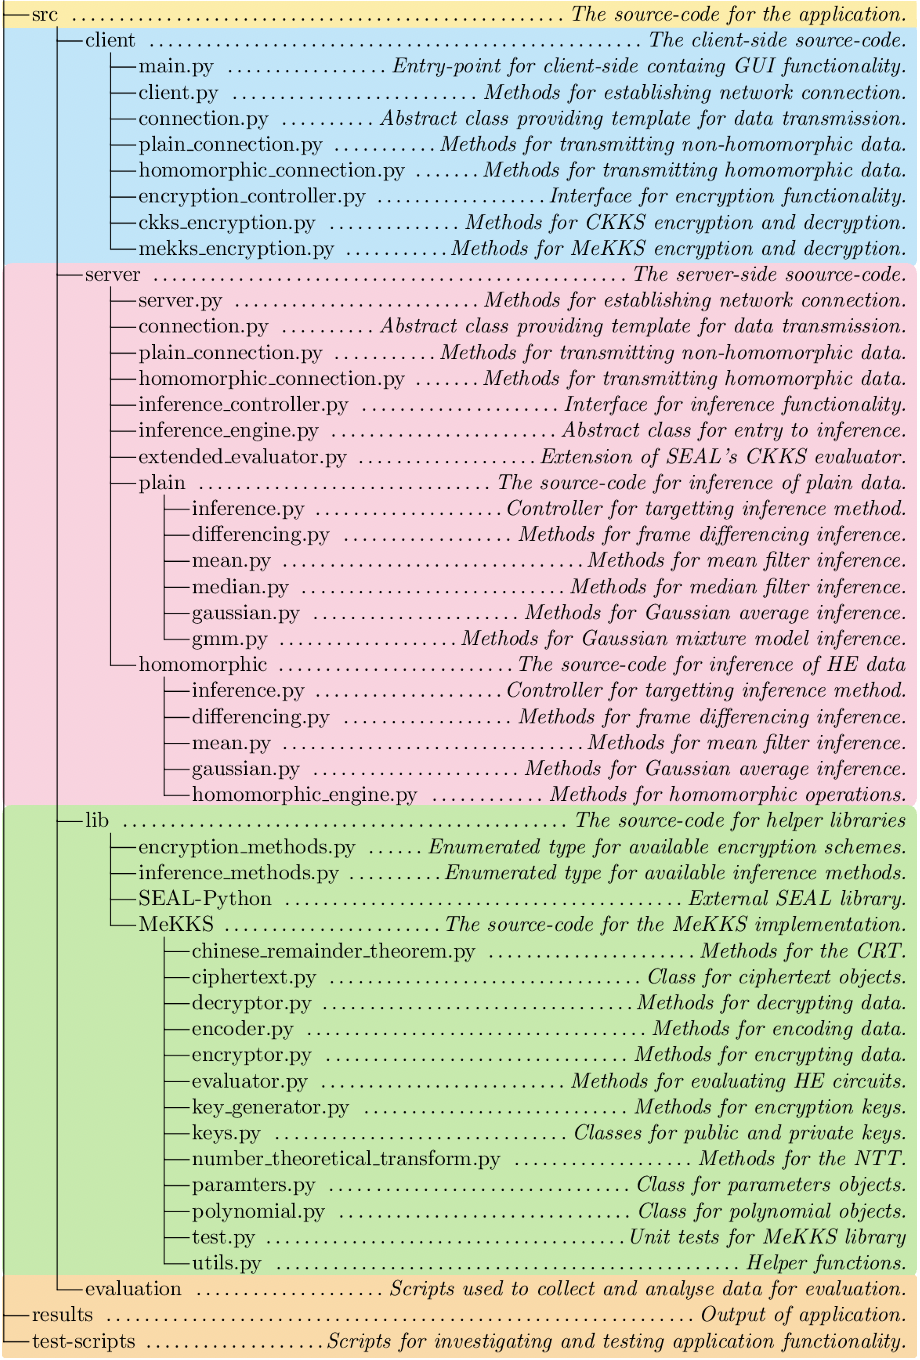
\includegraphics[scale=0.97]{figures/repositoryOverview}
    \caption[Repository Overview]{Repository Overview.}
    \label{fig:filetree}
\end{figure}
\setlength{\leftskip}{0cm}
\subsection{Class Structure}
\setlength{\leftskip}{0.5cm}
\indent \indent
This section provides a more thorough insight into the project's structure. Figure \ref{fig:clientUML} details the arrangement of the client-side, Figure \ref{fig:serverUML} contains the classes composing the server-side, and Figure \ref{fig:mekksUML} depicts the structure of the MeKKS library. While there is overlap in these class diagrams, they have been separated into three figures for the sake of clarity.

\begin{figure}[htp]
    \centering
    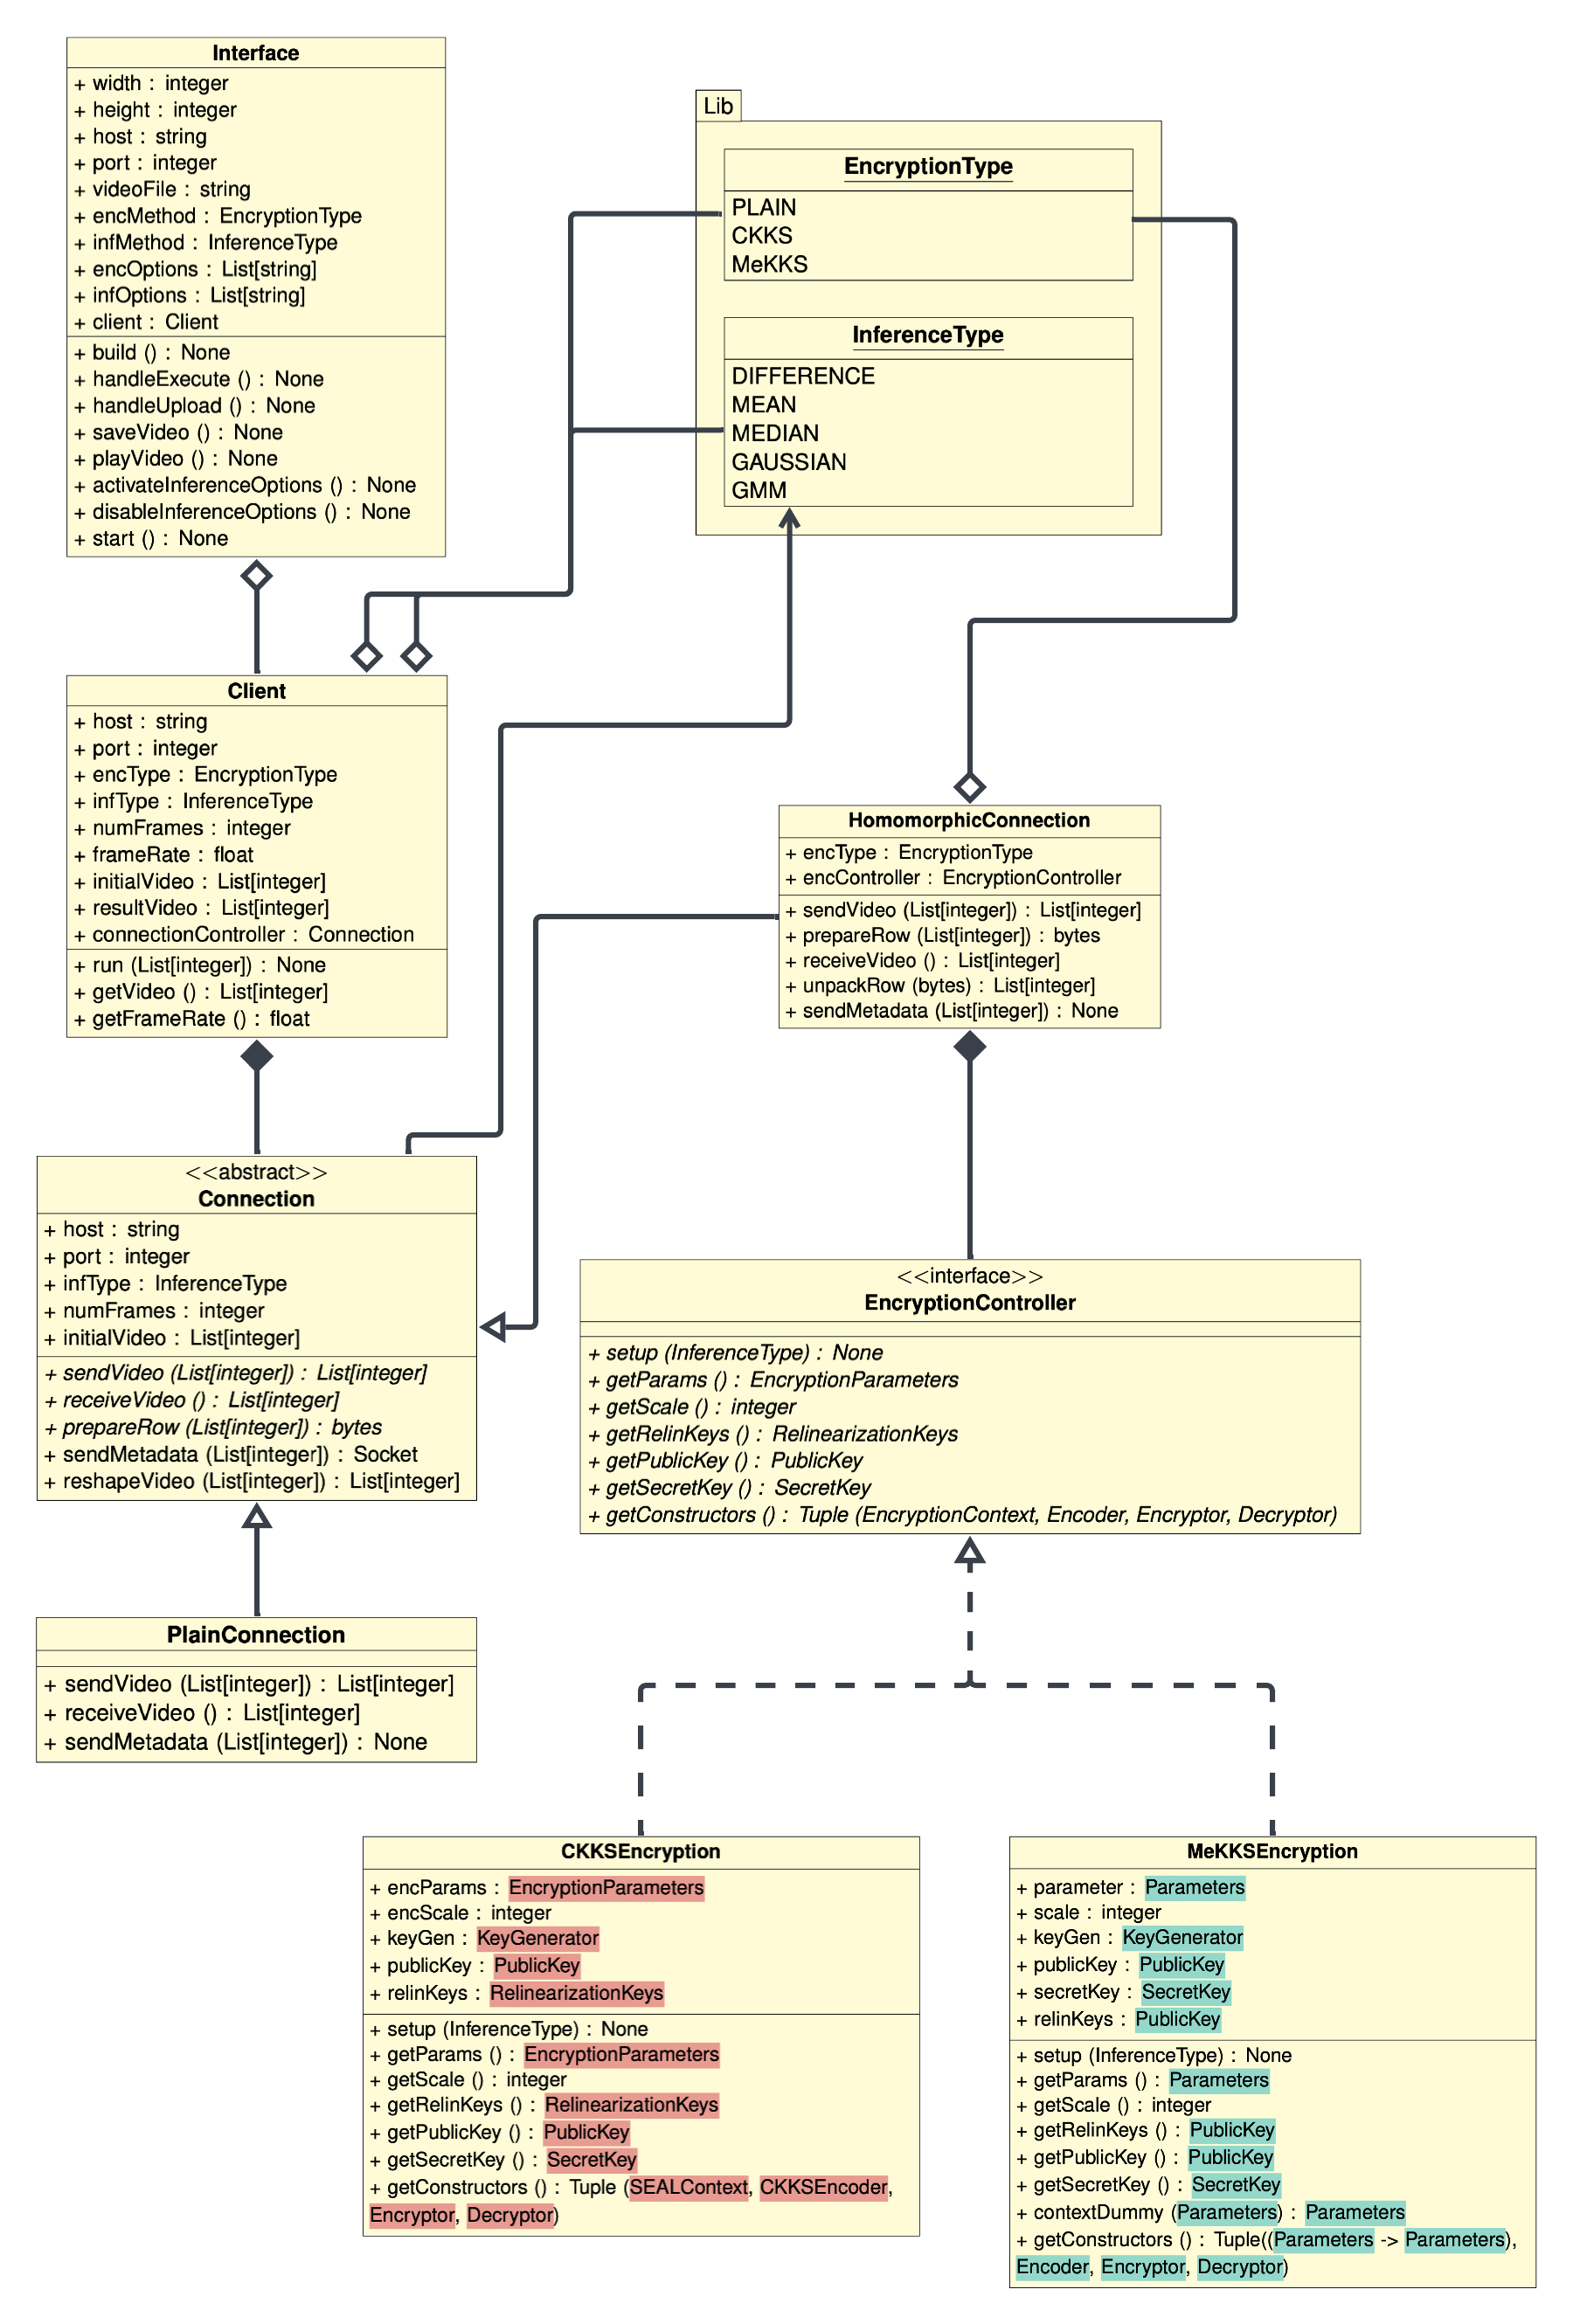
\includegraphics[scale=0.24]{figures/clientClasses}
    \captionsetup{justification=centering}
    % \scalebox{0.6}{\begin{tikzpicture}
    \begin{class}[text width=7cm]{Interface}{-3.5,10}
        \attribute{+ width : integer}
        \attribute{+ height : integer}
        \attribute{+ host : string}
        \attribute{+ port : integer}
        \attribute{+ videoFile : string}
        \attribute{+ encMethod : EncryptionType}
        \attribute{+ infMethod : InferenceType}
        \attribute{+ encOptions : List[string]}
        \attribute{+ infOptions : List[string]}
        \attribute{+ client : Client}

        \operation{+ build () : None}
        \operation{+ handleExecute () : None}
        \operation{+ handleUpload () : None}
        \operation{+ saveVideo () : None}
        \operation{+ playVideo () : None}
        \operation{+ activateInferenceOptions () : None}
        \operation{+ disableInferenceOptions () : None}
        \operation{+ start () : None}
    \end{class}


    \begin{class}[text width=7cm]{Client}{-3.5,-2}
        \attribute{+ host : string}
        \attribute{+ port : integer}
        \attribute{+ encType : EncryptionType}
        \attribute{+ infType : InferenceType}
        \attribute{+ numFrames : integer}
        \attribute{+ frameRate : float}
        \attribute{+ initialVideo : List[integer]}
        \attribute{+ resultVideo : List[integer]}
        \attribute{+ connectionController : Connection}
        
        \operation{+ run (List[integer]) : None}
        \operation{+ getVideo () : List[integer]}
        \operation{+ getFrameRate () : float}
    \end{class}

    
    \begin{abstractclass}[text width=8cm]{Connection}{-3.2,-11}
        \attribute{+ host : string}
        \attribute{+ port : integer}
        \attribute{+ infType : InferenceType}
        \attribute{+ numFrames : integer}
        \attribute{+ initialVideo : List[integer]}

        \operation{\textit{+ sendVideo (List[integer]) : List[integer]}}
        \operation{\textit{+ receiveVideo () : List[integer]}}
        \operation{\textit{+ prepareRow (List[integer]) : bytes}}
        \operation{+ sendMetadata (List[integer]) : Socket}
        \operation{+ reshapeVideo (List[integer]) : List[integer]}
    \end{abstractclass}

    
    \begin{class}[text width=7.5cm]{PlainConnection}{-3,-19}
        \operation{+ sendVideo (List[integer]) : List[integer]}
        \operation{+ receiveVideo () : List[integer]}
        \operation{+ sendMetadata (List[integer]) : None}
    \end{class}


    \begin{class}[text width=7.5cm]{HomomorphicConnection}{8,-3}
        \attribute{+ encType : EncryptionType}
        \attribute{+ encController : EncryptionController}
        
        \operation{+ sendVideo (List[integer]) : List[integer]}
        \operation{+ prepareRow (List[integer]) : bytes}
        \operation{+ receiveVideo () : List[integer]}
        \operation{+ unpackRow (bytes) : List[integer]}
        \operation{+ sendMetadata (List[integer]) : None}
    \end{class}


    \begin{interface}[text width=14.5cm]{EncryptionController}{14,-10}
        \operation{\textit{+ setup (InferenceType) : None}}
        \operation{\textit{+ getParams () : EncryptionParameters}}
        \operation{\textit{+ getScale () : integer}}
        \operation{\textit{+ getRelinKeys () : RelinearizationKeys}}
        \operation{\textit{+ getPublicKey () : PublicKey}}
        \operation{\textit{+ getSecretKey () : SecretKey}}
        \operation{\textit{+ getConstructors () : Tuple (EncryptionContext, Encoder, Encryptor, Decryptor)}}
    \end{interface}


    \begin{class}[text width=11cm]{CKKSEncryption}{8.3,-26}
        \sethlcolor{ckksRed}
        \attribute{+ encParams : \hl{EncryptionParameters}}
        \attribute{+ encScale : integer}
        \attribute{+ keyGen : \hl{KeyGenerator}}
        \attribute{+ publicKey : \hl{PublicKey}}
        \attribute{+ relinKeys : \hl{RelinearizationKeys}}

        \operation{+ setup (InferenceType) : None}
        \operation{+ getParams () : \hl{EncryptionParameters}}
        \operation{+ getScale () : integer}
        \operation{+ getRelinKeys () : \hl{RelinearizationKeys}}
        \operation{+ getPublicKey () : \hl{PublicKey}}
        \operation{+ getSecretKey () : \hl{SecretKey}}
        \operation{+ getConstructors () : Tuple (\hl{SEALContext}, \hl{CKKSEncoder}, \hl{Encryptor}, \hl{Decryptor})}
    \end{class}


    \begin{class}[text width=10.5cm]{MeKKSEncryption}{17,-16}
        \sethlcolor{mekksBlue}
        \attribute{+ parameter : \hl{Parameters}}
        \attribute{+ scale : integer}
        \attribute{+ keyGen : \hl{KeyGenerator}}
        \attribute{+ publicKey : \hl{PublicKey}}
        \attribute{+ secretKey : \hl{SecretKey}}
        \attribute{+ relinKeys : \hl{PublicKey}}

        \operation{+ setup (InferenceType) : None}
        \operation{+ getParams () : \hl{Parameters}}
        \operation{+ getScale () : integer}
        \operation{+ getRelinKeys () : \hl{PublicKey}}
        \operation{+ getPublicKey () : \hl{PublicKey}}
        \operation{+ getSecretKey () : \hl{SecretKey}}
        \operation{+ contextDummy (\hl{Parameters}) : \hl{Parameters}}
        \operation{+ getConstructors () : Tuple((\hl{Parameters} -> \hl{Parameters}), \hl{Encoder}, \hl{Encryptor}, \hl{Decryptor})}
    \end{class}


    \begin{package}{Lib}
        \begin{object}[text width=7cm]{EncryptionType}{12,6}
            \attribute{PLAIN}
            \attribute{CKKS}
            \attribute{MeKKS}
        \end{object}


        \begin{object}[text width=7cm]{InferenceType}{12,3}
            \attribute{DIFFERENCE}
            \attribute{MEAN}
            \attribute{MEDIAN}
            \attribute{GAUSSIAN}
            \attribute{GMM}
        \end{object}
    \end{package}

    % \begin{scope}[line width=0.8mm]
    %     \aggregation{Interface}{}{}{Client}
    %     \path (Interface) -- (Client) node[pos=0.7,right]{\large 1};

    %     \composition{Client}{}{}{Connection}
    %     \path (Client) -- (Connection) node[pos=0.7,right]{\large 1};

    %     \draw[>=open triangle 60,->] (PlainConnection) to (Connection);

    %     \draw[>=open triangle 60,->] (HomomorphicConnection) to (Connection);

    %     \composition{HomomorphicConnection}{}{}{EncryptionController}
    %     \path (HomomorphicConnection) -- (EncryptionController) node[pos=0.8, right]{\large 1};

    %     \draw[>=open triangle 60,dashed,->] (EncryptionController) to (CKKSEncryption);

    %     \draw[>=open triangle 60,dashed,->] (EncryptionController) to (MeKKSEncryption);

    %     \unidirectionalAssociation{Client}{}{}{EncryptionType}

    %     \unidirectionalAssociation{Client}{}{}{InferenceType}

    %     \unidirectionalAssociation{Connection}{}{}{InferenceType}

    %     \unidirectionalAssociation{HomomorphicConnection}{}{}{EncryptionType}
    % \end{scope}
\end{tikzpicture}

}
    \caption[Client UML Class Diagram]{UML Class Diagram showing the components of the client side.\medskip\\External CKKS classes:\sethlcolor{ckksRed} \hl{\quad\quad\quad\quad}\smallskip\\External MeKKS classes:\sethlcolor{mekksBlue} \hl{\quad\quad\quad\quad}}
    \label{fig:clientUML}
\end{figure}
        
\begin{figure}[htp]
    \centering
    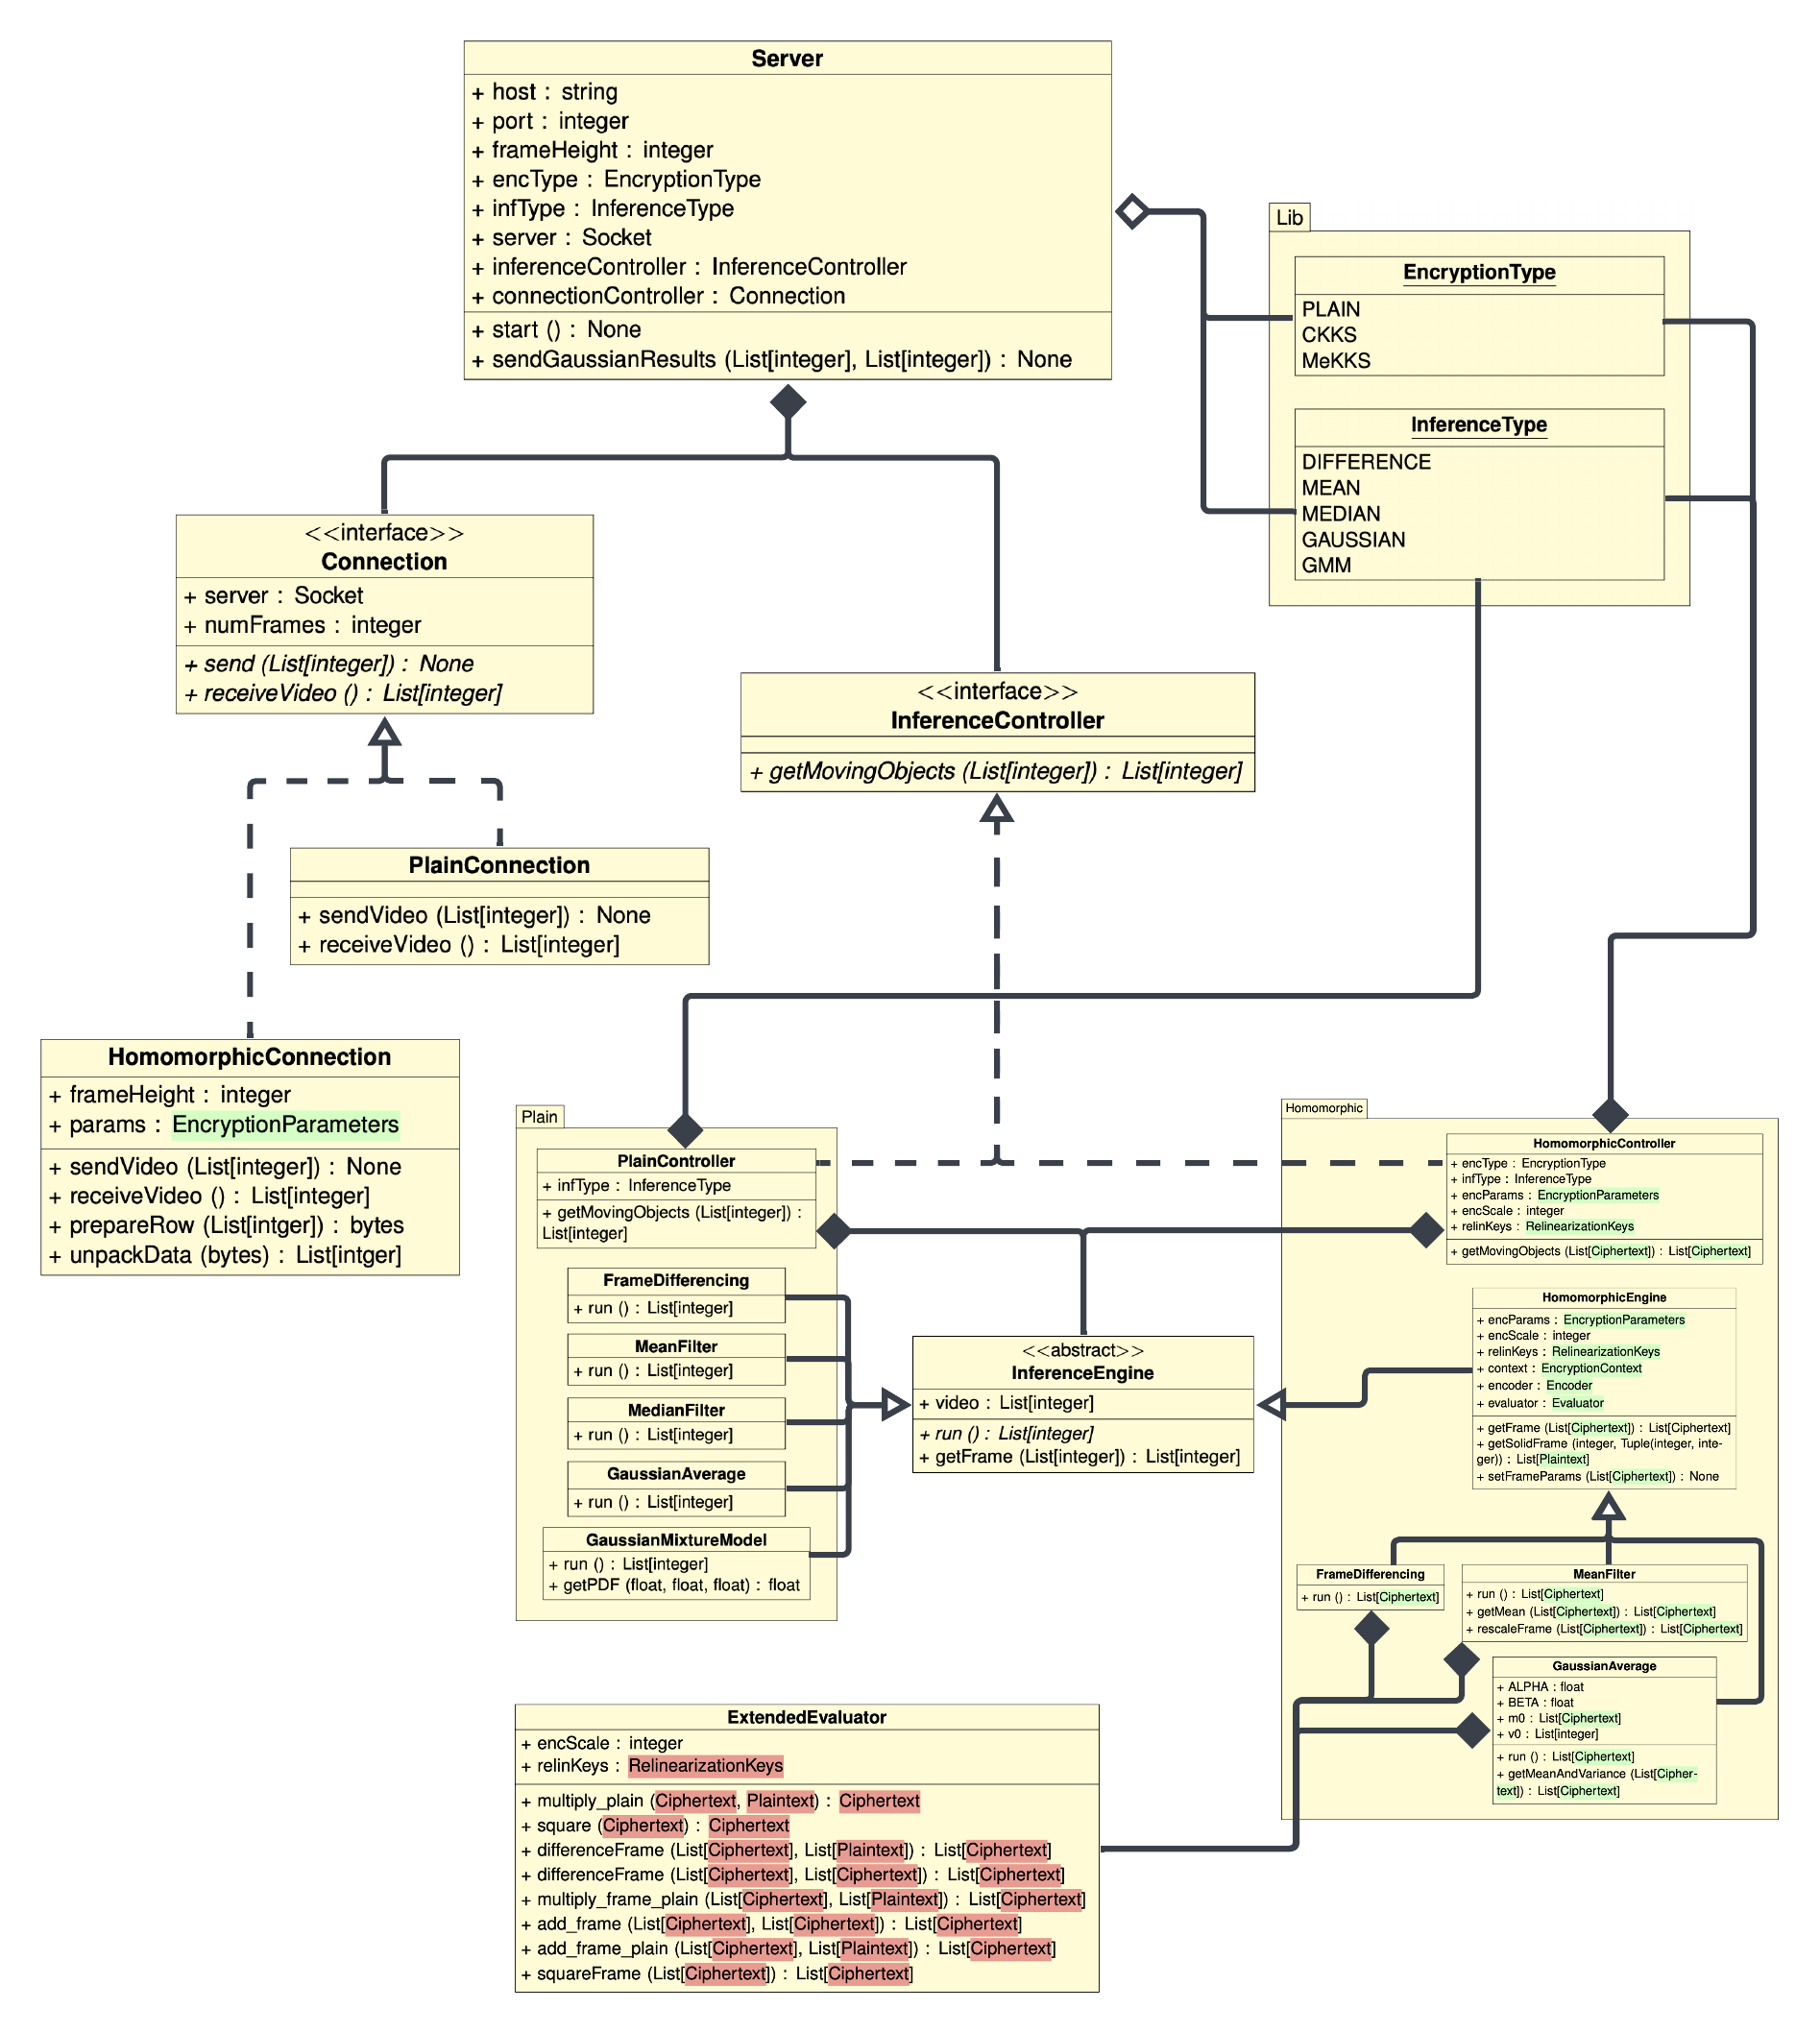
\includegraphics[scale=0.236]{figures/serverClasses}
    \captionsetup{justification=centering}
    % \scalebox{0.6}{\input{figures/serverClasses}}
    \caption[Client UML Class Diagram]{UML Class Diagram showing the components of the server side.\medskip\\External CKKS classes:\sethlcolor{ckksRed} \hl{\quad\quad\quad\quad}\smallskip\\Abstract HE objects:\sethlcolor{homomorphicGreen} \hl{\quad\quad\quad\quad}}
    \label{fig:serverUML}
\end{figure}
        
\begin{figure}[htp]
    \centering
    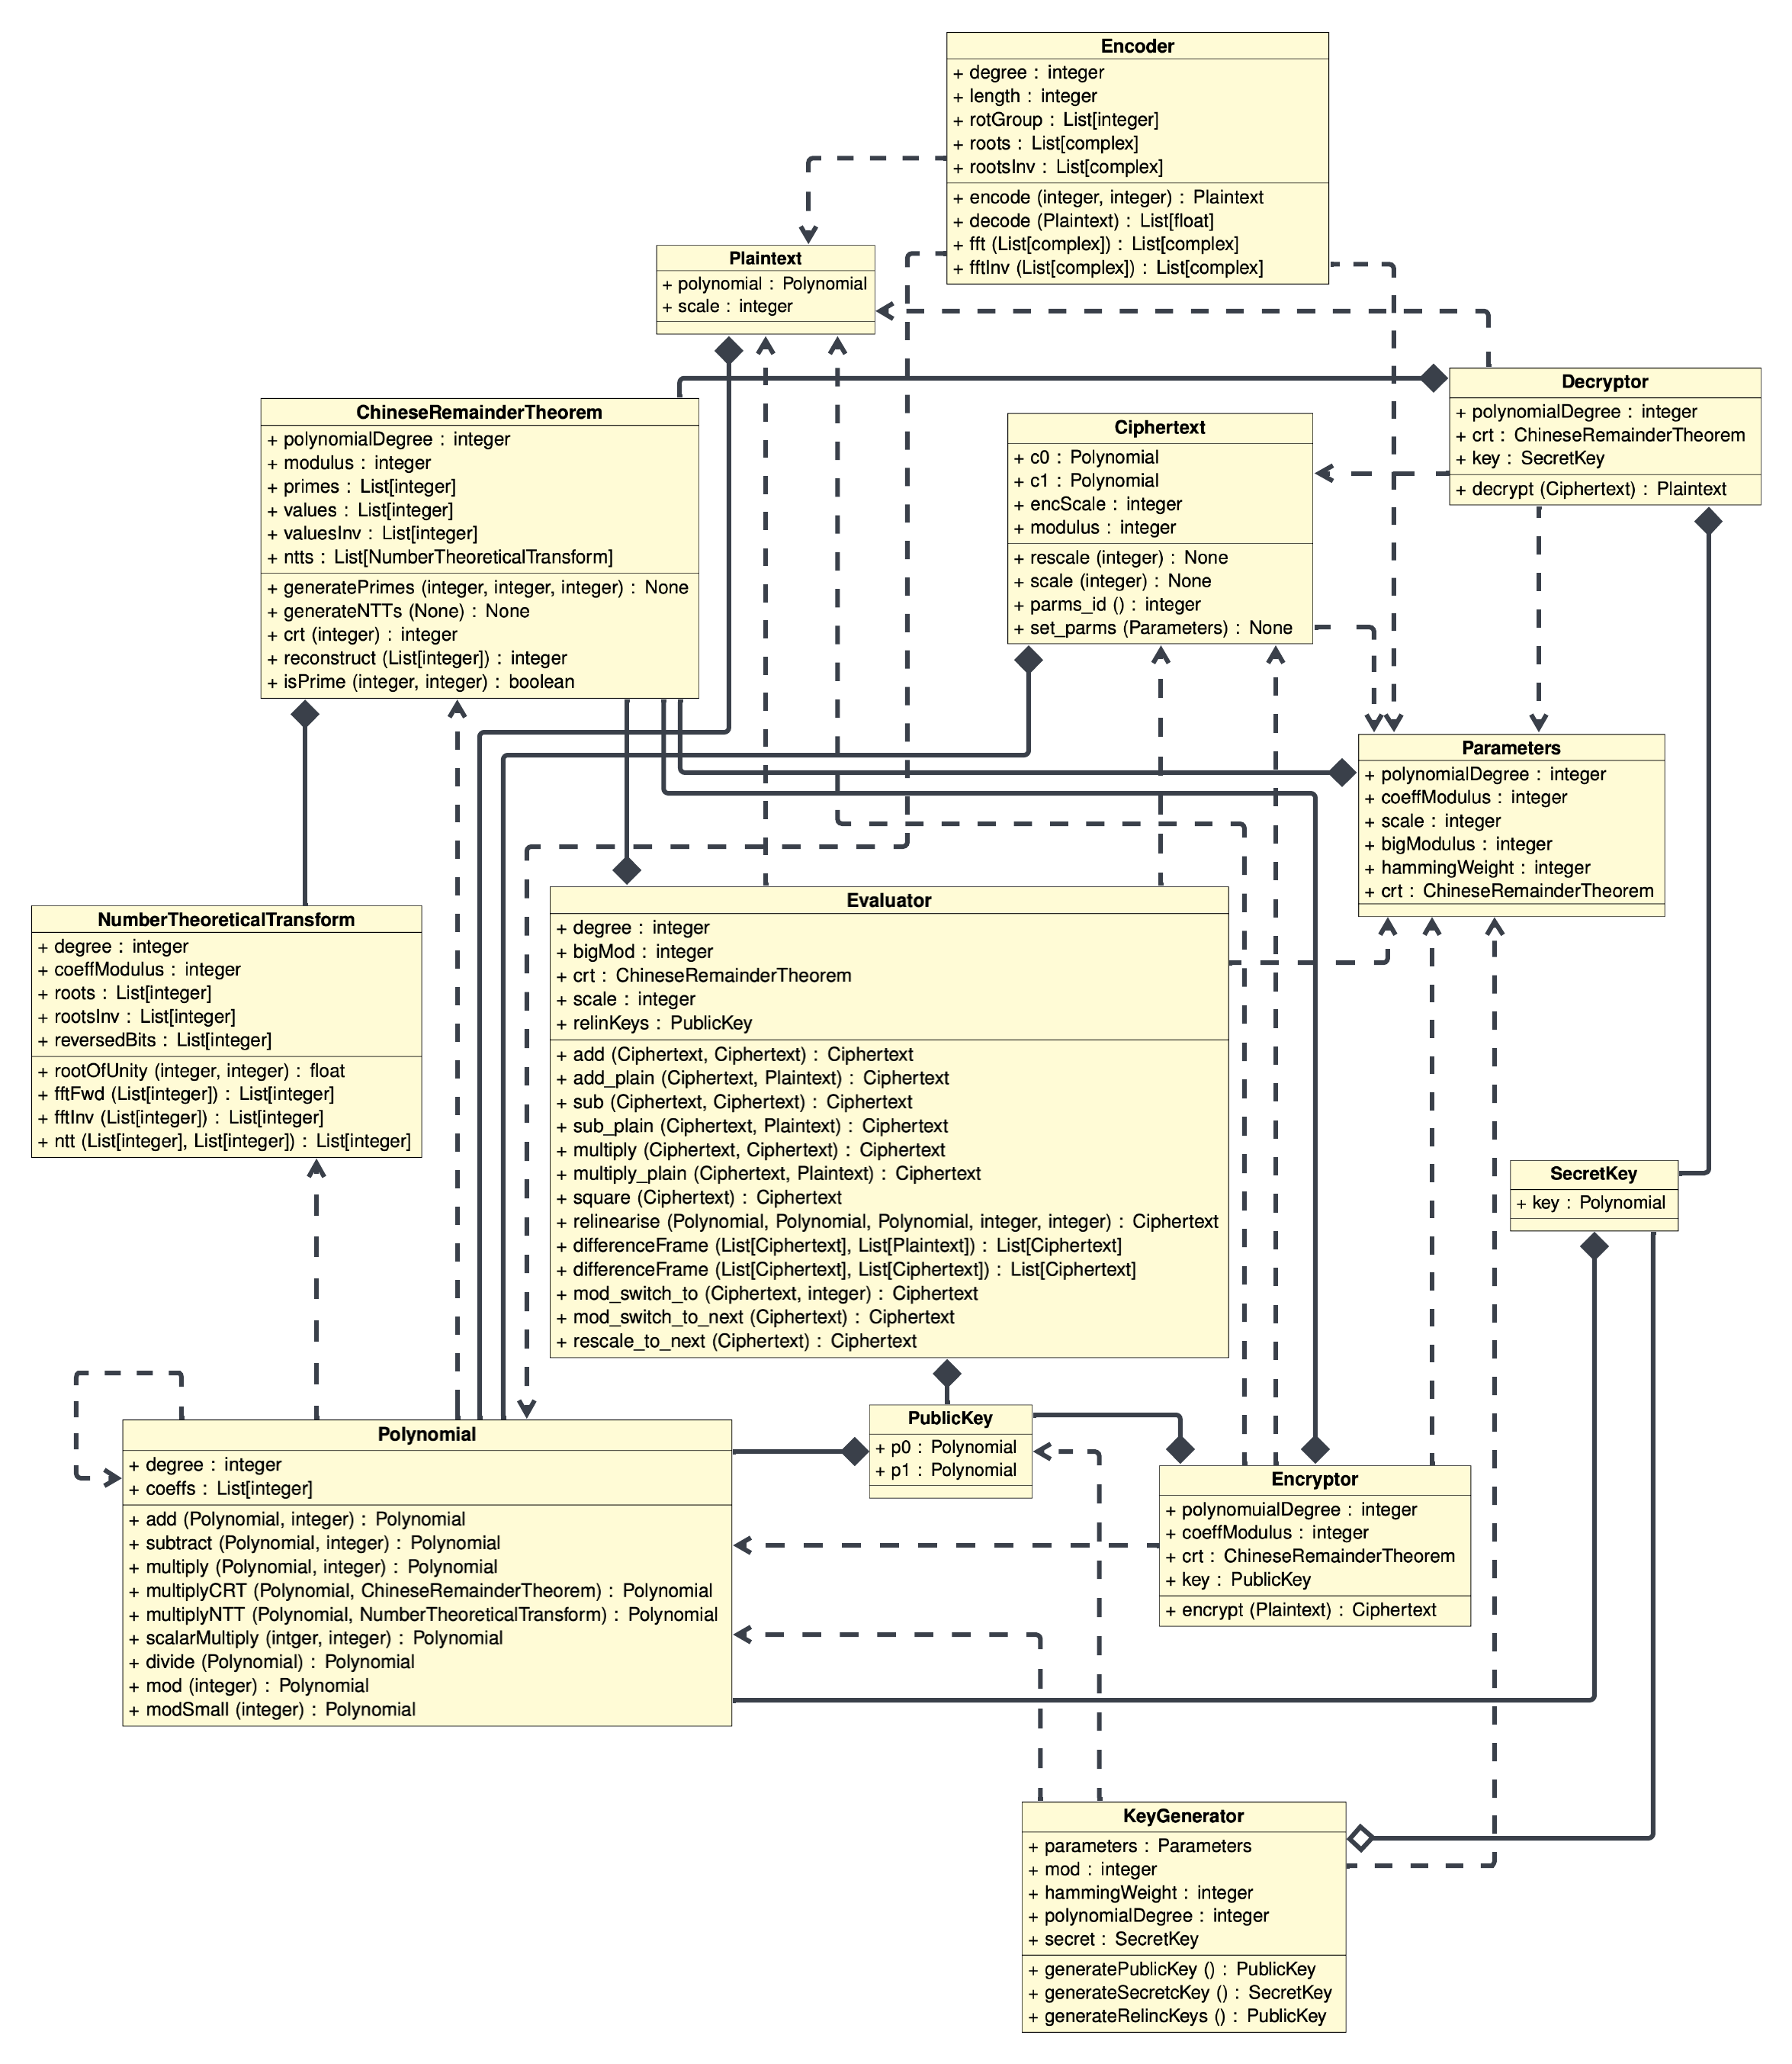
\includegraphics[scale=0.19]{figures/mekksClasses}
    \captionsetup{justification=centering}
    % \scalebox{0.6}{\begin{tikzpicture}
    \begin{class}[text width=9.2cm]{ChineseRemainderTheorem}{0,0}
        \attribute{+ polynomialDegree : integer}
        \attribute{+ modulus : integer}
        \attribute{+ primes : List[integer]}
        \attribute{+ values : List[integer]}
        \attribute{+ valuesInv : List[integer]}
        \attribute{+ ntts : List[NumberTheoreticalTransform]}

        \operation{+ generatePrimes (integer, integer, integer) : None}
        \operation{+ generateNTTs (None) : None}
        \operation{+ crt (integer) : integer}
        \operation{+ reconstruct (List[integer]) : integer}
        \operation{+ isPrime (integer, integer) : boolean}
    \end{class}


    \begin{class}[text width=6.4cm]{Ciphertext}{9, 0}
        \attribute{+ c0 : Polynomial}
        \attribute{+ c1 : Polynomial}
        \attribute{+ encScale : integer}
        \attribute{+ modulus : integer}

        \operation{+ rescale (integer) : None}
        \operation{+ scale (integer) : None}
        \operation{+ parms\_id () : integer}
        \operation{+ set\_parms (Parameters) : None}
    \end{class}


    \begin{class}[text width=6.5cm]{Decryptor}{9,-6}
        \attribute{+ polynomialDegree : integer}
        \attribute{+ crt : ChineseRemainderTheorem}
        \attribute{+ key : SecretKey}

        \operation{+ decrypt (Ciphertext) : Plaintext}
    \end{class}


    \begin{class}[text width=8cm]{Encoder}{0,-8}
        \attribute{+ degree : integer}
        \attribute{+ length : integer}
        \attribute{+ rotGroup : List[integer]}
        \attribute{+ roots : List[complex]}
        \attribute{+ rootsInv : List[complex]}

        \operation{+ encode (integer, integer) : Plaintext}
        \operation{+ decode (Plaintext) : List[float]}
        \operation{+ fft (List[complex]) : List[complex]}
        \operation{+ fftInv (List[complex]) : List[complex]}
    \end{class}


    \begin{class}[text width=6.5cm]{Encryptor}{0,-20}
        \attribute{+ polynomuialDegree : integer}
        \attribute{+ coeffModulus : integer}
        \attribute{+ crt : ChineseRemainderTheorem}
        \attribute{+ key : PublicKey}

        \operation{+ encrypt (Plaintext) : Ciphertext}
    \end{class}


    % \begin{class}[text width=14.2cm]{Evaluator}{-3,-14}
    %     \attribute{+ degree : integer}
    %     \attribute{+ bigMod : integer}
    %     \attribute{+ crt : ChineseRemainderTheorem}
    %     \attribute{+ scale : integer}
    %     \attribute{+ relinKeys : PublicKey}

    %     \operation{+ add (Ciphertext, Ciphertext) : Ciphertext}
    %     \operation{+ add\_plain (Ciphertext, Plaintext) : Ciphertext}
    %     \operation{+ sub (Ciphertext, Ciphertext) : Ciphertext}
    %     \operation{+ sub\_plain (Ciphertext, Plaintext) : Ciphertext}
    %     \operation{+ multiply (Ciphertext, Ciphertext) : Ciphertext}
    %     \operation{+ multiply\_plain (Ciphertext, Plaintext) : Ciphertext}
    %     \operation{+ square (Ciphertext) : Ciphertext}
    %     \operation{+ relinearise (Polynomial, Polynomial, Polynomial, integer, integer) : Ciphertext}
    %     \operation{+ differenceFrame (List[Ciphertext], List[Plaintext]) : List[Ciphertext]}
    %     \operation{+ differenceFrame (List[Ciphertext], List[Ciphertext]) : List[Ciphertext]}
    %     \operation{+ mod\_switch\_to (Ciphertext, integer) : Ciphertext}
    %     \operation{+ mod\_switch\_to\_next (Ciphertext) : Ciphertext}
    %     \operation{+ rescale\_to\_next (Ciphertext) : Ciphertext}
    % \end{class}


    \begin{class}[text width=6.8cm]{KeyGenerator}{0,-14}
        \attribute{+ parameters : Parameters}
        \attribute{+ mod : integer}
        \attribute{+ hammingWeight : integer}
        \attribute{+ polynomialDegree : integer}
        \attribute{+ secret : SecretKey}

        \operation{+ generatePublicKey () : PublicKey}
        \operation{+ generateSecretcKey () : SecretKey}
        \operation{+ generateRelincKeys () : PublicKey}
    \end{class}


    \begin{class}[text width=3.4cm]{PublicKey}{9, -20}
        \attribute{+ p0 : Polynomial}
        \attribute{+ p1 : Polynomial}
    \end{class}


    \begin{class}[text width=3.5cm]{SecretKey}{9, -23}
        \attribute{+ key : Polynomial}
    \end{class}

    \begin{class}[text width=8.2cm]{NumberTheoreticalTransform}{18, 0}
        \attribute{+ degree : integer}
        \attribute{+ coeffModulus : integer}
        \attribute{+ roots : List[integer]}
        \attribute{+ rootsInv : List[integer]}
        \attribute{+ reversedBits : List[integer]}

        \operation{+ rootOfUnity (integer, integer) : float}
        \operation{+ fftFwd (List[integer]) : List[integer]}
        \operation{+ fftInv (List[integer]) : List[integer]}
        \operation{+ ntt (List[integer], List[integer]) : List[integer]}
    \end{class}


    \begin{class}[text width=6.4cm]{Parameters}{9, -25}
        \attribute{+ polynomialDegree : integer}
        \attribute{+ coeffModulus : integer}
        \attribute{+ scale : integer}
        \attribute{+ bigModulus : integer}
        \attribute{+ hammingWeight : integer}
        \attribute{+ crt : ChineseRemainderTheorem}
    \end{class}


    \begin{class}[text width=4.7cm]{Plaintext}{18,-7}
        \attribute{+ polynomial : Polynomial}
        \attribute{+ scale : integer}
    \end{class}


    \begin{class}[text width=12.8cm]{Polynomial}{18,-10}
        \attribute{+ degree : integer}
        \attribute{+ coeffs : List[integer]}

        \operation{+ add (Polynomial, integer) : Polynomial}
        \operation{+ subtract (Polynomial, integer) : Polynomial}
        \operation{+ multiply (Polynomial, integer) : Polynomial}
        \operation{+ multiplyCRT (Polynomial, ChineseRemainderTheorem) : Polynomial}
        \operation{+ multiplyNTT (Polynomial, NumberTheoreticalTransform) : Polynomial}
        \operation{+ scalarMultiply (intger, integer) : Polynomial}
        \operation{+ divide (Polynomial) : Polynomial}
        \operation{+ mod (integer) : Polynomial}
        \operation{+ modSmall (integer) : Polynomial}
    \end{class}
\end{tikzpicture}
}
    \caption[MeKKS UML Class Diagram]{UML Class Diagram showing the components of the MeKKS encryption scheme.}
    \label{fig:mekksUML}
\end{figure}

\setlength{\leftskip}{0cm}





\section{Encryption}
\setlength{\leftskip}{0.25cm}
\indent \indent
This section briefly discusses the fundamentals of the CKKS HE scheme, as described in the original paper by Cheon et al.\ ~\cite{CKKS}, and how it is implemented in this project.  Also, to provide further insights and an investigation in specialising HE schemes, a bespoke CKKS implementation is detailed, called MeKKS. 

\setlength{\leftskip}{0cm}
\subsection{CKKS Primitives}
\label{sec:CKKS}
\setlength{\leftskip}{0.5cm}
\indent \indent
Fundamentally, the CKKS scheme encrypts plaintext polynomials into ciphertext polynomials. Addition and multiplication operations can then be performed on the data, introducing uncertainty to the values. Finally, ciphertext polynomials can be decrypted to retrieve approximations of plaintext polynomials, with the accuracy depending on the number of operations performed.
\smallskip \\ \indent
Therefore, to encrypt vectors of real values, they must be first be encoded as polynomials in the ring $\mathcal{R} = \mathbb{Z}[X] / (X^N + 1)$, where $N$ is a power of 2. During encoding, the real values must be rounded. To preserve precision, the vector is multiplied by a \textit{scaling factor}, $\Delta$. Once the vector has been encoded into a polynomial in $\mathcal{R}$, it can be encrypted into a \textit{pair} of polynomials: the ciphertext.
\smallskip \\ \indent
Consider two vectors $\vec{v}$ and $\vec{w}$. To encode these vectors, they are scaled to $\Delta \vec{v}$ and $\Delta \vec{w}$.  They can then be encrypted and multiplied to give ciphertext equivalents of $\Delta^2 (\vec{v} \bigodot \vec{w})$. It is clear from this that a sequence of multiplication operations will continue to increase the scale factor indefinitely. To overcome this, CKKS introduces a \textit{rescaling} procedure, which can be understood as dividing the ciphertext by $\Delta$ to reduce the scale.
\smallskip \\ \indent
However, rescaling is not a free operation, so it cannot be continuously applied to allow unlimited multiplications. CKKS is a levelled HE scheme, so each ciphertext resides at a discrete level. Each level has a coefficient modulus $q$ that dictates a ciphertext's coefficients must be in $\mathbb{Z}_q$. When a polynomial is first encrypted, it exists in the maximum level, $L$, with coefficient modulus $Q = q_0 \dot \Delta^L$, for a \textit{base modulus} $q_0$. When a ciphertext is rescaled, the coefficient modulus is divided by $\Delta$, reducing it to $q_0 \cdot \Delta^{L-1}$. Hence, the ciphertext is lowered to the next level. If a ciphertext reaches level 0, no further multiplications can be applied, to preserve the encrypted values. For correct decryption, the coefficients of a polynomial cannot exceed $q_0$. Consequently, in practice, $q_0$ is much larger than $\Delta$.

\setlength{\leftskip}{0cm}
\subsubsection{Encoding and Decoding}
\setlength{\leftskip}{0.5cm}
\indent \indent
In CKKS, the plaintext message space is the \textit{cyclotomic polynomial ring} $\mathcal{R} = \mathbb{Z}[X] / \Phi_M(X)$, where $\Phi_M(X)$ is the $M$-th cyclotomic polynomial and $M$ is a power of two. Encoding is the process of mapping a complex vector to an element in $\mathcal{R}$, and decoding is the process of reversing this mapping.
\smallskip \\ \indent
Another way of defining decoding is as a mapping of an element $r \in \mathcal{R}$ to a vector in $\mathbb{C}^N$ using the embedding $\sigma : \frac{\mathbb{R}[X]}{X^N + 1} \rightarrow \mathbb{C}^N$. This is applied to each root of $\Phi_M(X)$ through the evaluation of $r$ as
\begin{equation}
    \sigma(r) = (r(\xi), r(\xi^3), \ldots, r(\xi^{M-1})) = (r(\xi^k) \: | \: k \in \mathbb{Z}^*_N) \in \mathbb{C}^N
\end{equation}
where $\xi = e^{\frac{2 \pi i}{M}}$ is a primitive $M$-th root of unity.
\smallskip \\ \indent
However, to establish a one-to-one mapping, the input must be \textit{scaled} and \textit{rounded} during encoding, and half of the complex vector must be \textit{discarded} during decoding.
\smallskip \\ \indent
As a result of the above, the CKKS encoding function has the form given in Equation \ref{eq:encode}.
\begin{equation}
    \label{eq:encode}
    \texttt{Encode}(\vec{v}, \Delta) : \mathbb{C}^\frac{N}{2} \times \mathbb{Z}^+ \rightarrow \mathcal{R}
\end{equation}

\setlength{\leftskip}{0cm}
\subsubsection{Operations}
\setlength{\leftskip}{0.5cm}
\indent \indent
Figure \ref{fig:ckksOps} lists the operations supported by CKKS and their definitions. An important observation is the multiplication of polynomials required during ciphertext multiplication. This makes multiplication a much more computationally expensive operation than addition.
\begin{figure}[ht]
    \centering
    \begin{tcolorbox}
        \begin{itemize}[leftmargin=0.1cm]
            \item \texttt{KeyGen} : sample $s \leftarrow \chi_{\text{key}}$, $\vec{r}' \rightarrow \mathcal{R}_{qL}$, $\vec{r}' \rightarrow \mathcal{R}_{P \cdot qL}$, $\vec{e} \leftarrow \chi_{\text{err}}$, and $\vec{e}' \leftarrow \chi_{\text{err}}$.
            \begin{enumerate}
                \item Calculate $\vec{a} := - \vec{r} \vec{s} + \vec{e} \mod q_L$ and $\vec{a}' := -\vec{r}' \vec{s} + \vec{e}' + P \vec{s}^2 \mod P \cdot qL$.
                \item Return $\texttt{SecretKey} := (1, \vec{s})$, $\texttt{PublicKey} := (\vec{a}, \vec{r})$, $\texttt{EvaluationKey} := (\vec{a}', \vec{r}')$.
            \end{enumerate}
            \item $\texttt{Enc}_\texttt{PublicKey}(\vec{m})$ : sample $\vec{v} \leftarrow \chi_{\text{enc}}$ and $\vec{e}_0, \vec{e}_1 \leftarrow \chi_{\text{err}}$.
            \begin{enumerate}
                \item Calculate $\vec{c}_0 := \vec{v} \cdot \vec{a} + \vec{m} + \vec{e}_0$ and $\vec{c}_1 := \vec{v} \cdot \vec{r} + \vec{e}_1$.
                \item Return $(\vec{c}_0, \vec{c}_1) \mod q_L$.
            \end{enumerate}
            \item $\texttt{Dec}_\texttt{SecretKey}(\vec{c}_0 + \vec{c}_1 \cdot \vec{s}) = (\vec{c}_0 + \vec{c}_1) \mod q_l$.
            \item $\texttt{Add}((\vec{c}_0, \vec{c}_1), (\vec{d}_0, \vec{d}_1)) = (\vec{c}_0 + \vec{d}_0, \vec{c}_1 + \vec{d}_1) \mod q_l$.
            \item $\texttt{AddPlain}((\vec{c}_0, \vec{c}_1), x) = (c_0 + \texttt{Enc}_\texttt{PublicKey}(x), \vec{c}_1) \mod q_l$.
            \item $\texttt{Multiply}((\vec{c}_0, \vec{c}_1), (\vec{d}_0, \vec{d}_1)) = (\vec{r}_0, \vec{r}_1) + (\lfloor P^{-1} \cdot \vec{r}_2 \cdot \texttt{EvaluationKey}_0 \rceil, \lfloor P^{-1} \cdot \vec{r}_2 \cdot \texttt{EvaluationKey}_1  \rceil) \mod q_l$.
            \item $\texttt{MultiplyPlain}((\vec{c}_0, \vec{c}_1), x) = (\vec{c}_0 \cdot \texttt{Enc}_\texttt{PublicKey}(x), \vec{c}_1 \cdot \texttt{Enc}_\texttt{PublicKey}(x)) \mod q_l$.
        \end{itemize}
    \end{tcolorbox}
    \caption[CKKS Operations]{A list of the basic operations supported by the CKKS scheme. $P$ is a large scaling factor and $\lfloor \cdot \rceil$ denotes rounding to the nearest integer. Recreated from \cite{CKKS}.}
    \label{fig:ckksOps}
\end{figure}

\setlength{\leftskip}{0cm}
\subsubsection{Rescaling}
\setlength{\leftskip}{0.5cm}
\indent \indent
The rescaling function introduced above is defined by equation \ref{eq:rescale}.
\begin{equation}
    \label{eq:rescale}
    \texttt{Rescale}(\vec{c}, \Delta^{l_\text{new}}) : \mathcal{R}^2_{ql} \times \mathbb{Z}^+ \rightarrow \mathcal{R}^2_{ql} = \lfloor \Delta^{l_\text{new} - l} \cdot \vec{c} \rceil \mod q_{l_\text{new}}
\end{equation}
Rescaling truncates some of the least-significant bits of a ciphertext by dividing by a power of the scaling factor. Practically, this is performed after every multiplication to revert the resulting $\Delta^2$ back down to just $\Delta$.  

\setlength{\leftskip}{0cm}
\subsubsection{Rotations}
\setlength{\leftskip}{0.5cm}
\indent \indent
An advantage of RLWE based HE schemes over others is the ability to \textit{rotate} ciphertext slots. Given a vector $\vec{V} = [v_0, v_1, v_2, \ldots, v_n]$ and an offset $d$. A rotation would cyclically shift each element by $d$ indices\footnote{For example, given $\vec{v} = [1, 2, 3, 4, 5]$ and $d = 2$ would produce $\vec{v}' = [4, 5, 1, 2, 3]$.}. This is achieved by homomorphically performing a \textit{Galois automorphism} on the ciphertext using standard results from \textit{Galois theory}. However, these operations are significantly the most expensive operations offered by RLWE-based schemes ~\cite{RotationBad}.

\setlength{\leftskip}{0cm}
\subsubsection{RNS Optimisations}
\setlength{\leftskip}{0.5cm}
\indent \indent
SEAL utilises a \textit{residue number system} \cite{RNS} to overcome the slow computations caused by very large polynomial coefficients requiring arbitrary precision arithmetic [RNS]. This exploits the Chinese Remainder Theorem (CRT) to decompose the coefficients in $\mathbb{Z}_q$ into $n$ smaller ones: $\mathbb{Z}_{p_1}, \ldots, \mathbb{Z}_{p_n}$. To do this, the CRT uses a \textit{moduli switching chain} $p_1, \ldots, p_n$ such that $\prod_i p_i = q$ and each $p_i$ is a prime number requiring fewer than 64-bits to store. Thanks to hardware limitations, it is faster to compute the $n$ separate multiplications in $p_1, \ldots, p_n$ than it is to compute a single multiplication in $q$. The results of the separate multiplications can be easily combined thanks to the isomorphism between $\mathbb{Z}_q$ and $\mathbb{Z}_{p_1}, \ldots, \mathbb{Z}_{p_n}$.
\smallskip \\ \indent
Unfortunately, as a result of the RNS optimisation, $q_l = q_0 \Delta^l$ cannot always be maintained due to the difficulty of finding every $q_l$ as the product of $n$ primes. To overcome this, SEAL instead defines $q_l = q_0 \prod_{i=1}^l p_i$ where $q_0$ must be prime. Where the original CKKS scheme divides by $\Delta$ to rescale, SEAL divides by $p_l$. Consequently, the resulting scaling factor is only approximately equal to $\Delta$. Therefore, in practice, the scaling factor must be manually reset to $\Delta$ after each multiplication and rescaling\footnote{Setting the scaling factor to $\Delta$ can be achieved by multiplying by a constant close to $1$, or using a ciphertexts \texttt{scale} function if $\Delta$ is known.}, and primes are chosen to be approximately the same size as $\Delta$.

\setlength{\leftskip}{0cm}

\subsection{MeKKS}
\label{sec:mekks}
\setlength{\leftskip}{0.5cm}
\indent \indent
Initially, the goal of implementing the CKKS scheme from first principles was to understand further the fundamental mathematical principles that allow it to work. There were little to no expectations of providing a performance improvement for the reasons detailed in §\ref{sec:mekksLimitations}. However, during the implementation phase, it became apparent that there may be some advantages to a specialised HE scheme that can overcome weaknesses found in SEAL during the earlier stages of development.

\setlength{\leftskip}{0cm}
\subsubsection{Limitations}
\label{sec:mekksLimitations}
\setlength{\leftskip}{0.5cm}
\indent \indent
The primary limitation of MeKKS was the language used for implementation. Traditionally, encryption schemes are written in C or C++ because they are lower-level than most languages, so they run more efficiently. Consequently, the more computationally expensive operations (such as the multiplications between large prime numbers required by CKKS, detailed above) would run much quicker than in Python. 
\smallskip \\ \indent
Another limitation was the number of optimisations that could be applied. Since the focus of the implementation was on understanding, the implementation began with the foundational CKKS scheme. However, since this scheme was released, many optimisations have been produced. For example, using residue number systems, bootstrapping extensions, or reduced approximation error ~\cite{RNS,BootstrappingHEAAN, RAE}. The opportunities for developing MeKKS are extensive. However, it was essential to define a clear endpoint for the implementation for the sake of scheduling the project and the inflexible final deadline. Therefore, the performance expectations compared to SEAL - which has had years of development from a team of experts - were further bounded.

\setlength{\leftskip}{0cm}
\subsubsection{Implementation}
\setlength{\leftskip}{0.5cm}
\indent \indent
The first iteration of MeKKS implementation began using the scheme outlined by Cheon et al. in 2016. This allowed all of the functionality described in §\ref{sec:CKKS} to be implemented, and the API constructed following SEAL to allow for easy integration into the core application.
\smallskip \\ \indent
However, the performance of this implementation meant it was infeasible to integrate into the rest of the application. Therefore, the next iteration of the HEAAN paper was used to add a bootstrapping procedure, dramatically speeding up computation ~\cite{BootstrappingHEAAN}. Taking advantage of the \textit{approximate computation} characteristic of this encryption scheme, the bootstrapping approach aims to evaluate the decryption formula approximately so that an encryption of the original message can be obtained in a large ciphertext modulus. Hence, an approximation of the \textit{modular reduction} formula is implemented such that it can be efficiently evaluated using standard HE arithmetic operations - where the error induced by the approximation is small enough to maintain precision.
\smallskip \\ \indent
Using the observation that the modular reduction function, $F(t) = [t]_q$, is the identity nearby zero and periodic in $q$, bootstrapping uses a trigonometric function to approximate the function when $t = \langle \texttt{Ciphertext}, \texttt{SecretKey} \rangle$ is close to a multiple of $q$ (the ciphertext modulus). Specifically, using the \textit{sine} function in the formula given by Equation \ref{eq:bootstrapping}.
\begin{equation}
    \label{eq:bootstrapping}
    [\langle \texttt{Ciphertext}, \texttt{SecretKey} \rangle]_q = \frac{q}{2 \pi} \cdot \sin \left( \frac{2 \pi}{q} \cdot \langle \texttt{Ciphertext}, \texttt{SecretKey} \rangle \right) + O(\epsilon^3 \cdot q)
\end{equation}
when $F(\langle \texttt{Ciphertext}, \texttt{SecretKey} \rangle) < \epsilon \cdot q$.
\smallskip \\ \indent
The Taylor polynomial can be used to approximate the trigonometric function so that it can be calculated in the HE domain. The input, $t$, is bounded by $K \cdot q$ for some constant $K = O(\lambda)$, where $\lambda$ is the security parameter. The degree of the Taylor polynomial should be at least $O(K \cdot q)$ in order to make the error term small enough on the interval $(-K \cdot q, K \cdot q)$. Cheon et al.\ proposed using the \textit{Paterson-Stockmeyer} method to reduce the complexity of these calculations ~\cite{BootstrappingHEAAN, Paterson}. However, the complexity of recryption grows exponentially with the depth of the decryption circuit, which still has a substantial impact.
\smallskip \\ \indent
Figure \ref{fig:bootstrapping} provides a graphical representation of the bootstrapping approximation.
\begin{figure}[ht]
    \centering
    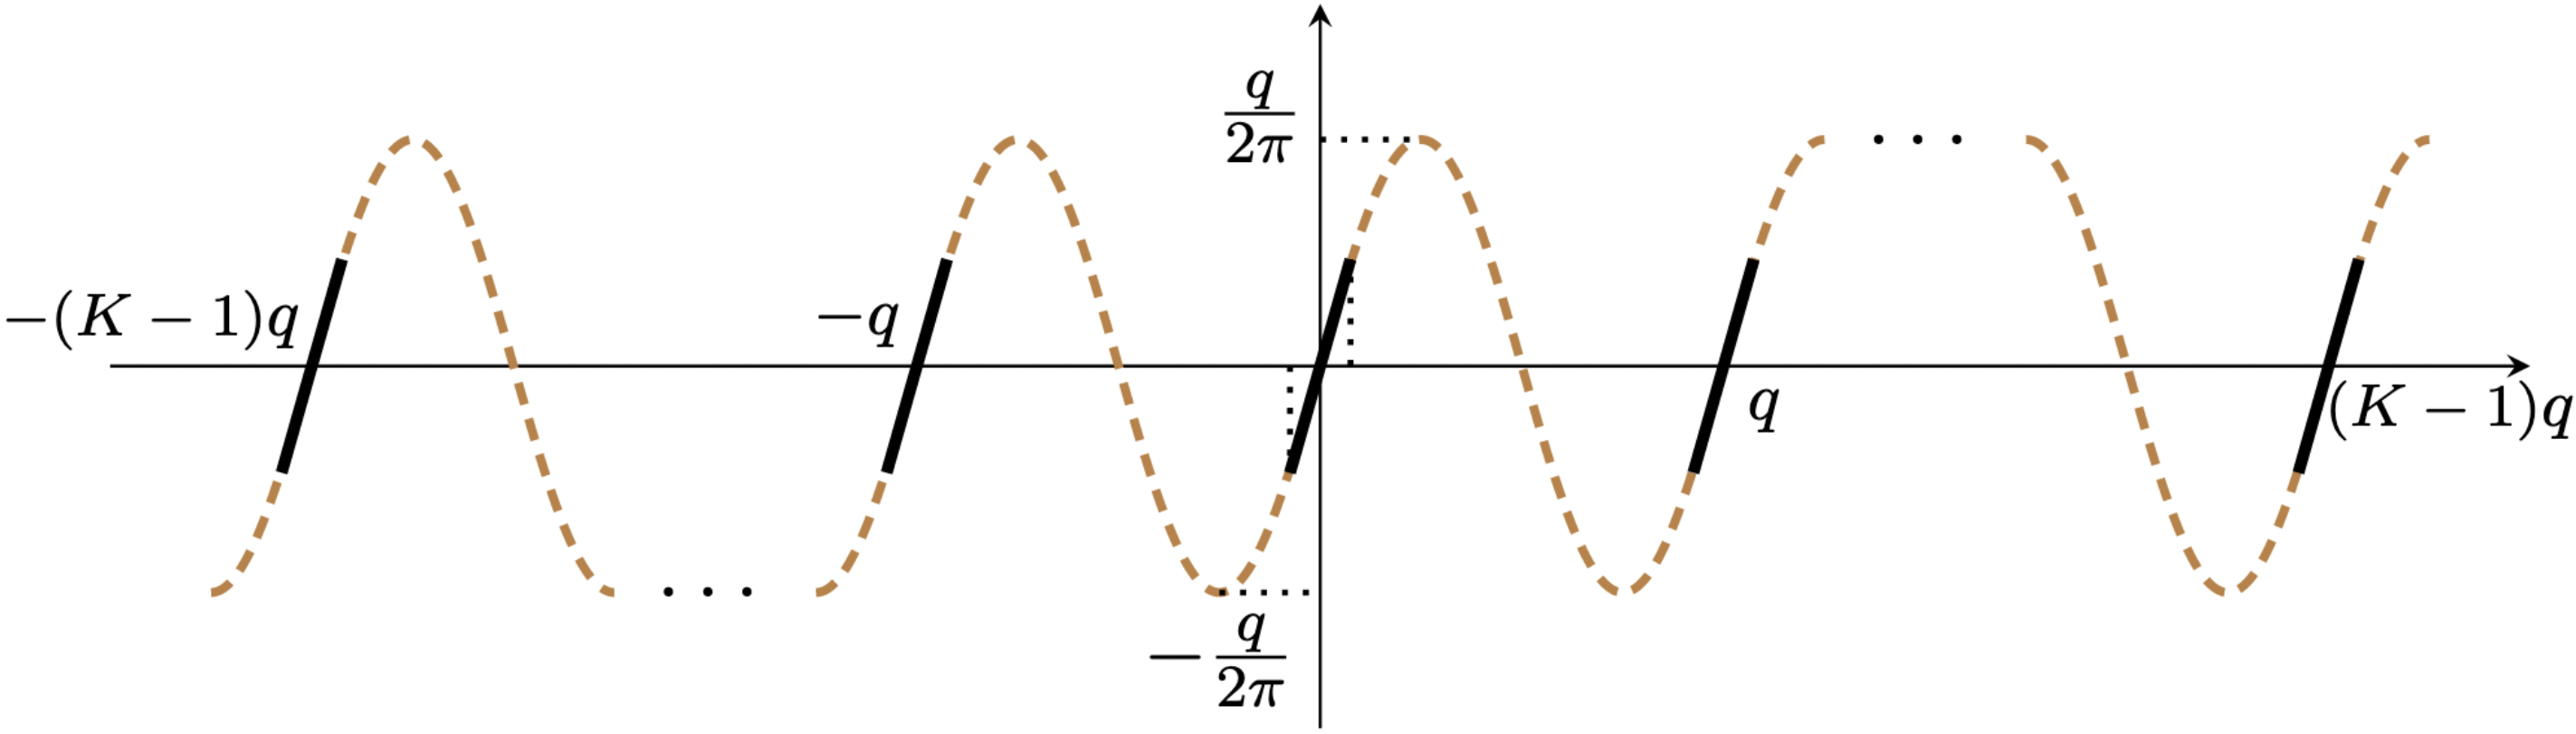
\includegraphics[scale=0.3]{figures/bootstrapping.png}
    \caption[Bootstrapping Procedure]{Modular Reduction and Scaled Sine Functions. Reproduced from \cite{BootstrappingHEAAN}.}
    \label{fig:bootstrapping}
\end{figure}

\setlength{\leftskip}{0cm}
\subsubsection{Optimisations}
\setlength{\leftskip}{0.5cm}
\indent \indent
The principal optimisations of MeKKS came through the methods of data representation. When integrating SEAL into the project, a Python wrapper for a C++ implementation was used. Consequently, the application was forced to handle large C++ objects, hidden by a further layer of abstraction via the wrapper. Therefore, Python struggled to manipulate these objects efficiently, specifically during the networking stages of execution. As explained in §\ref{sec:networking}, the bottleneck for SEAL's performance was in data serialisation. However, since MeKKS was written in Python, the underlying functionality provided much more efficient manipulation as it could directly interact with the objects and their attributes.
\smallskip \\ \indent
Another optimisation came through the specialisation of the library. The project planning ensured MeKKS was only implemented once the application's core had been complete. As a result, the functionality required had been investigated and almost wholly finalised. Therefore, only the components needed for each class in MeKKS were implemented. This further reduced the size of objects and removed any unnecessary computations, making execution more efficient. For example, the most expensive operations offered by SEAL are rotations. However, since the application did not use them, they were ignored during the implementation of MeKKS.

\setlength{\leftskip}{0cm}



\section{Networking}
\label{sec:networking}
\setlength{\leftskip}{0.25cm}
\indent \indent
This section is dedicated to detailing the techniques investigated for tackling the networking portion of the project. An established limitation of HE is its impact on memory usage ~\cite{Makkaoui}. Consequently, the \textit{transmission time} of data is significantly impaired. Given a video file, the \textit{transmission time} can be defined by Equation \ref{eq:transmission}.
\begin{equation}
    \text{transmission time} = \frac{\text{video size }\textit{(bytes)}}{\text{transmission rate }\textit{(bytes/second)}}
    \label{eq:transmission}
\end{equation}
\indent \indent
The core design of this project focused on emulating the MLaaS model employed by surveillance technology companies. Therefore, transferring large volumes of data to the cloud is a critical component, so a substantial portion of the investigation was considering how to reduce the effect of HE on uploading videos. The problem was considered from two angles: attempting to reduce the \textit{video size} (see §\ref{sec:seamCarving} and §\ref{sec:graphReps}) and attempting to increase the \textit{transmission rate} (see §\ref{sec:parallelisation}).

\setlength{\leftskip}{0cm}
\subsection{Memory Requirements}
\subsubsection{Seam Carving}
\label{sec:seamCarving}
\setlength{\leftskip}{0.5cm}
\indent \indent
Developed by Avidan and Shamir in 2007, \textit{seam carving} describes a method of resizing images using \textit{geometric constraints} while also considering \textit{image content} ~\cite{SeamCarving}. The advantage of accounting for both aspects is that an image can be resized to some target dimensions while preserving important features, such as people or buildings. There are two categories of methods for distinguishing these features. Firstly, \textit{top-down} methods use tools such as \textit{face detectors} to highlight were the features appear in the image ~\cite{Viola}. Whereas a \textit{bottom-up} approach uses \textit{saliency maps}\footnote{a representation highlighting the regions of an image where a persons' eyes are first drawn, see \cite{Saliency}.} to locate the most important ~\cite{Itti}.
\smallskip \\ \indent
However, instead of focussing on the most critical pixels of an image, seam carving targets the least important - those that ``won't be noticed'' if removed. To do this, it defines an \textit{energy function} for each pixel in an image. The original paper proposes multiple energy functions, beginning with the function shown in Equation \ref{eq:energy1} before developing Equation \ref{eq:energy2}.
\begin{equation}
    \label{eq:energy1}
    e(\vec{I}) = \left| \frac{\partial}{\partial x} \vec{I} \right| + \left| \frac{\partial}{\partial y} \vec{I} \right|
\end{equation}
\begin{equation}
    \label{eq:energy2}
    e_{\textit{HoG}}(\vec{I}) = \frac{\left| \frac{\partial}{\partial x} \vec{I} \right| + \left| \frac{\partial}{\partial y} \vec{I} \right|}{\max{(\textit{HoG}(\vec{I}(x,y)))}}
\end{equation}
where $\textit{HoG}(\vec{I}(x,y))$ is a histogram of oriented gradients at every pixel. The paper recommended an eight-bin histogram over an eleven-pixel square window around each pixel. Figure \ref{fig:scEnergy} depicts the application of an energy function to an example image.
\smallskip \\ \indent
Once the energy of each pixel has been calculated, the image can be split into \textit{seams}. A \textit{vertical seam} is a path of pixels connecting the top of an image to the bottom, such that there is only a single pixel from each column in the path. A \textit{horizontal seam} is a path of pixels connecting the left of an image to the right, such that there is only a single pixel from each column in the path. Formally, this is defined by Equation \ref{eq:vSeam} and Equation \ref{eq:hSeam} for vertical and horizontal seams respectively.
\begin{subequations}
    \begin{equation}
        \label{eq:vSeam}
        \vec{s}^\vec{x} = \{s^x_i\}^n_{i=1} = \{(x(i), i) \: s.t. \: \forall i \: |x(i) - x(i-1)| \leq 1\}^n_{i=1}
    \end{equation}
    \begin{equation}
        \label{eq:hSeam}
        \vec{s}^\vec{y} = \{s^y_j\}^m_{j=1} = \{(j, y(j)) \: s.t. \: \forall j \: |y(j) - y(j-1)| \leq 1\}^m_{j=1}
    \end{equation}
\end{subequations}
For an $n \times m$ image, \vec{I}, where $x : [1, \ldots, n] \rightarrow [1, \ldots, m]$ and $y : [1, \ldots, m] \rightarrow [1, \ldots, n]$. Figure \ref{fig:scSeams} depicts generating seams from pixel energies.
\smallskip \\ \indent
From this set, the \textit{optimal seam} is found. That is, the seam that minimises the \textit{seam cost} in Equation \ref{eq:seamCost}. Some implementations will calculate this seam using a variant of Dijkstra's algorithm, but a more common method is to use dynamic programming to implement Equation \ref{eq:dpSeamCarving} (for vertical seams - the definition of $M$ for horizontal seams is similar).
\begin{equation}
    \label{eq:seamCost}
    E(\vec{s}) = E(\vec{I_s}) = \sum^n_{i=1} = e(\vec{I}(s_i))
\end{equation}
\begin{equation}
    \label{eq:dpSeamCarving}
    M(i, j) = e(i,j) + \min{(M(i-1, j-1), M(i-1, j), M(i-1, j+1))}
\end{equation}
\indent
Building on the original algorithm, this project implements the \textit{forward energy} function developed by Rubinstein et al.\ ~\cite{Rubinstein}. Another dynamic programming algorithm, forward energy, improves the selection of the optimal seam in iteration $i$ by accounting for the impact on energy in the iteration $i+1$ of the algorithm and iteration $i$. To do this, the \textit{energy difference} function is defined by Equation \ref{eq:energyDiff}, where $C$ is the cost of removing the seam. 
\begin{equation}
    \label{eq:energyDiff}
    \Delta E_{i+1} = E(\vec{I}_{i+1}) - (E(\vec{I}_i) - E(C_i))
\end{equation}
\indent
Consequently, this criterion looks forward to the resulting image to search for the seam, which would inject minimal energy. The cost of removing a seam is measured as the forward differences between the pixels that become neighbours once the seam is removed. There are three cases for this, the pixels are diagonally adjacent in either direction, or the pixels are orthogonally adjacent, as demonstrated by Figure \ref{fig:adjacency} and formalised by Equation \ref{eq:adjacency}. From this, the Equation \ref{eq:dpSeamCarving} can be updated to become Equation \ref{eq:forwardEnergy}.
\begin{figure}[htp]
    \scalebox{0.78}{\begin{tikzpicture}
    \node (aT) at (0,0) [draw,line width=0.5mm,minimum width=6cm,minimum height=4cm] {};
    \node (aT1) at (-2,-1) [draw,line width=0.25mm,minimum width=2cm,minimum height=2cm] {\large$p_{i,j-1}$};
    \node (aT2) at (0,-1) [draw,line width=0.25mm,minimum width=2cm,minimum height=2cm,fill=ckksRed] {\large$p_{i,j}$};
    \node (aT3) at (2,-1) [draw,line width=0.25mm,minimum width=2cm,minimum height=2cm] {\large$p_{i,j+1}$};
    \node (aT4) at (-2,1) [draw,line width=0.25mm,minimum width=2cm,minimum height=2cm,fill=ckksRed] {\large$p_{i-1,j-1}$};
    \node (aT5) at (0,1) [draw,line width=0.25mm,minimum width=2cm,minimum height=2cm] {\large$p_{i-1,j}$};
    \node (aT6) at (2,1) [draw,line width=0.25mm,minimum width=2cm,minimum height=2cm] {\large$p_{i-1,j+1}$};

    \draw[->,>=stealth,line width=1.5mm] ([xshift=0.5cm,yshift=0.5cm]aT4.south) to ([xshift=-0.5cm,yshift=-0.5cm]aT2.north);

    \node (aB) at (0,-6) [draw,line width=0.5mm,minimum width=4cm,minimum height=4cm] {};
    \node (aB1) at (-1,-7) [draw,line width=0.25mm,minimum width=2cm,minimum height=2cm,fill=mekksBlue] {\large$p_{i,j-1}$};
    \node (aB2) at (1,-7) [draw,line width=0.25mm,minimum width=2cm,minimum height=2cm,fill=mekksBlue] {\large$p_{i,j+1}$};
    \node (aB3) at (-1,-5) [draw,line width=0.25mm,minimum width=2cm,minimum height=2cm,fill=mekksBlue] {\large$p_{i-1,j}$};
    \node (aB3) at (1,-5) [draw,line width=0.25mm,minimum width=2cm,minimum height=2cm,fill=mekksBlue] {\large$p_{i-1,j+1}$};

    \draw[-,line width=1.5mm,color=red] ([xshift=-1cm]aB1.north) to ([xshift=-0.925cm]aB2.north);
    \draw[-,line width=1.5mm,color=red] ([xshift=1cm]aB1.south) to ([xshift=-1cm]aB2.north);

    \draw[->,>=stealth,line width=2mm] ([yshift=-0.25cm]aT.south) to ([yshift=0.25cm]aB.north);

    \node at (0, 3) {\LARGE\textbf{\textrm{L}}};




    \node (bT) at (7,0) [draw,line width=0.5mm,minimum width=6cm,minimum height=4cm] {};
    \node (bT1) at (5,-1) [draw,line width=0.25mm,minimum width=2cm,minimum height=2cm] {\large$p_{i,j-1}$};
    \node (bT2) at (7,-1) [draw,line width=0.25mm,minimum width=2cm,minimum height=2cm,fill=ckksRed] {\large$p_{i,j}$};
    \node (bT3) at (9,-1) [draw,line width=0.25mm,minimum width=2cm,minimum height=2cm] {\large$p_{i,j+1}$};
    \node (bT4) at (5,1) [draw,line width=0.25mm,minimum width=2cm,minimum height=2cm] {\large$p_{i-1,j-1}$};
    \node (bT5) at (7,1) [draw,line width=0.25mm,minimum width=2cm,minimum height=2cm,fill=ckksRed] {\large$p_{i-1,j}$};
    \node (bT6) at (9,1) [draw,line width=0.25mm,minimum width=2cm,minimum height=2cm] {\large$p_{i-1,j+1}$};

    \draw[->,>=stealth,line width=1.5mm] ([yshift=0.5cm]bT5.south) to ([yshift=-0.5cm]bT2.north);

    \node (bB) at (7,-6) [draw,line width=0.5mm,minimum width=4cm,minimum height=4cm] {};
    \node (bB1) at (6,-7) [draw,line width=0.25mm,minimum width=2cm,minimum height=2cm,fill=mekksBlue] {\large$p_{i,j-1}$};
    \node (bB2) at (8,-7) [draw,line width=0.25mm,minimum width=2cm,minimum height=2cm,fill=mekksBlue] {\large$p_{i,j+1}$};
    \node (bB3) at (6,-5) [draw,line width=0.25mm,minimum width=2cm,minimum height=2cm,fill=mekksBlue] {\large$p_{i-1,j-1}$};
    \node (bB3) at (8,-5) [draw,line width=0.25mm,minimum width=2cm,minimum height=2cm,fill=mekksBlue] {\large$p_{i-1,j+1}$};

    \draw[-,line width=1.5mm,color=red] ([xshift=1cm]bB1.south) to ([xshift=-1cm]bB2.north);

    \draw[->,>=stealth,line width=2mm] ([yshift=-0.25cm]bT.south) to ([yshift=0.25cm]bB.north);

    \node at (7, 3) {\LARGE\textbf{\textrm{U}}};



    \node (cT) at (14,0) [draw,line width=0.5mm,minimum width=6cm,minimum height=4cm] {};
    \node (cT1) at (12,-1) [draw,line width=0.25mm,minimum width=2cm,minimum height=2cm] {\large$p_{i,j-1}$};
    \node (cT2) at (14,-1) [draw,line width=0.25mm,minimum width=2cm,minimum height=2cm,fill=ckksRed] {\large$p_{i,j}$};
    \node (cT3) at (16,-1) [draw,line width=0.25mm,minimum width=2cm,minimum height=2cm] {\large$p_{i,j+1}$};
    \node (cT4) at (12,1) [draw,line width=0.25mm,minimum width=2cm,minimum height=2cm] {\large$p_{i-1,j-1}$};
    \node (cT5) at (14,1) [draw,line width=0.25mm,minimum width=2cm,minimum height=2cm] {\large$p_{i-1,j}$};
    \node (cT6) at (16,1) [draw,line width=0.25mm,minimum width=2cm,minimum height=2cm,fill=ckksRed] {\large$p_{i-1,j+1}$};

    \draw[->,>=stealth,line width=1.5mm] ([xshift=-0.5cm,yshift=0.5cm]cT6.south) to ([xshift=0.5cm,yshift=-0.5cm]cT2.north);

    \node (cB) at (14,-6) [draw,line width=0.5mm,minimum width=4cm,minimum height=4cm] {};
    \node (cB1) at (13,-7) [draw,line width=0.25mm,minimum width=2cm,minimum height=2cm,fill=mekksBlue] {\large$p_{i,j-1}$};
    \node (cB2) at (15,-7) [draw,line width=0.25mm,minimum width=2cm,minimum height=2cm,fill=mekksBlue] {\large$p_{i,j+1}$};
    \node (cB3) at (13,-5) [draw,line width=0.25mm,minimum width=2cm,minimum height=2cm,fill=mekksBlue] {\large$p_{i-1,j-1}$};
    \node (cB3) at (15,-5) [draw,line width=0.25mm,minimum width=2cm,minimum height=2cm,fill=mekksBlue] {\large$p_{i-1,j}$};

    \draw[-,line width=1.5mm,color=red] ([xshift=0.925cm]cB1.north) to ([xshift=1cm]cB2.north);
    \draw[-,line width=1.5mm,color=red] ([xshift=1cm]cB1.south) to ([xshift=-1cm]cB2.north);

    \draw[->,>=stealth,line width=2mm] ([yshift=-0.25cm]cT.south) to ([yshift=0.25cm]cB.north);

    \node at (14, 3) {\LARGE\textbf{\textrm{R}}};
    
\end{tikzpicture}
}
    \caption[Potential Seam Costs]{There are three possible vertical seam costs for pixel $(i, j)$. After removing the seam, new neighbours (blue) and new edges (red) are created.}. 
    \label{fig:adjacency}
\end{figure}
\begin{align}
    \label{eq:adjacency}
    \begin{split}
        C_L(i, j) &= |\vec{I}(i, j+1) - \vec{I}(i, j-1)| + |\vec{I}(i-1, j) - \vec{I}(i, j-1)|
    \end{split} \\
    \begin{split}
        C_U(i, j) &= |\vec{I}(i, j+1) - \vec{I}(i, j-1)|
    \end{split} \\
    \begin{split}
        C_R(i, j) &= |\vec{I}(i, j+1) - \vec{I}(i, j-1)| + |\vec{I}(i-1, j) - \vec{I}(i, j+1)|
    \end{split}
\end{align}
\begin{equation}
    \label{eq:forwardEnergy}
    M(i, j) = e(i, j) + \min 
    \begin{cases}
        M(i-1, j-1) + C_L(i,j) \\
        M(i-1, j) + C_U(i,j) \\
        M(i-1, j+1) + C_R(i,j)
    \end{cases}
\end{equation}
\indent
It is important to note that there have been several extensions to seam carving that may apply to this project. In particular, optimisations for videos by introducing two-dimensional seams to allow time to be accounted for, and implementations using GPUs to reduce execution time ~\cite{Rubinstein, Duarte}.


\begin{figure}[htp]
    \begin{subfloatrow}
        \floatbox[{\capbeside\thisfloatsetup{capbesideposition={right,center},capbesidewidth=3.7cm}}]{figure}[\FBwidth]
        {\caption{Original image.}}
        {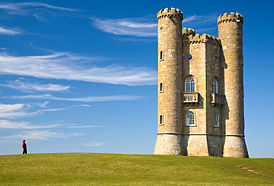
\includegraphics[scale=.7]{figures/seamCarving1.png}}
    \end{subfloatrow}
    \begin{subfloatrow}
        \floatbox[{\capbeside\thisfloatsetup{capbesideposition={right,center},capbesidewidth=5cm}}]{figure}[\FBwidth]
        {\caption{The energy of each pixel.}\label{fig:scEnergy}}
        {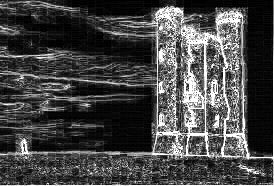
\includegraphics[scale=.7]{figures/seamCarving2.png}}
    \end{subfloatrow}
    \begin{subfloatrow}
        \floatbox[{\capbeside\thisfloatsetup{capbesideposition={right,center},capbesidewidth=5cm}}]{figure}[\FBwidth]
        {\caption{Potential seams to delete.}\label{fig:scSeams}}
        {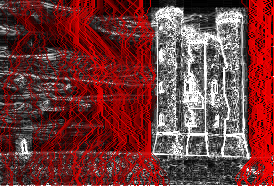
\includegraphics[scale=.7]{figures/seamCarving3.png}}
    \end{subfloatrow}
    \begin{subfloatrow}
        \floatbox[{\capbeside\thisfloatsetup{capbesideposition={right,center},capbesidewidth=11cm}}]{figure}[\FBwidth]
        {\caption{Low energy seams removed.}\label{fig:scRemoved}}
        {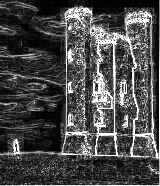
\includegraphics[scale=.7]{figures/seamCarving4.png}}
    \end{subfloatrow}
    \begin{subfloatrow}
        \floatbox[{\capbeside\thisfloatsetup{capbesideposition={right,center},capbesidewidth=9.5cm}}]{figure}[\FBwidth]
        {\caption{Resulting image.}}
        {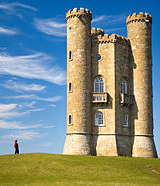
\includegraphics[scale=.7]{figures/seamCarving5.png}}
    \end{subfloatrow}
    \caption[Seam Carving Stages]{Each stage of the seam carving algorithm. Images taken from \cite{wikiSeamCarving}.}
\end{figure}

\setlength{\leftskip}{0cm}
\subsubsection{Graph Representation}
\label{sec:graphReps}
\setlength{\leftskip}{0.5cm}
\indent \indent
There are several advantages to representing an image using a graph. Firstly, graphs are discrete, mathematically simple objects that are well-suited to developing efficient, provably correct algorithms. Also, graph theory is a well-established research area with a wide variety of existing algorithms and theorems that can be utilised. More pertinent to this dissertation, graphs provide minimalistic representations of images that are flexible enough to account for different image types.
\smallskip \\ \indent
Graph-based image processing methods operate on \textit{pixel adjacency graphs}. More specifically, graphs whose vertex set is the set of image elements and edge set is given by an adjacency relation between image elements. A common approach to this uses the \textit{Euclidean adjacency relation} to define the edge set, formalised by Equation \ref{eq:adjacency}.
\begin{equation}
    d(v, w) \leq \rho
\end{equation}
for all vertices $v$, $w$ in the vertex set.  An example of some pixel adjacency graphs is given by Figure \ref{fig:pixelAdjacency}. When handling video files, three-dimensional pixel adjacency graphs are used to account for relationships between video frames. An example of these is depicted by Figure \ref{fig:3dAdjacency}.
\begin{figure}[h!]
    \centering
    \begin{subfigure}[b]{0.29\textwidth}
        \centering
        \captionsetup{justification=centering}
        \scalebox{1}{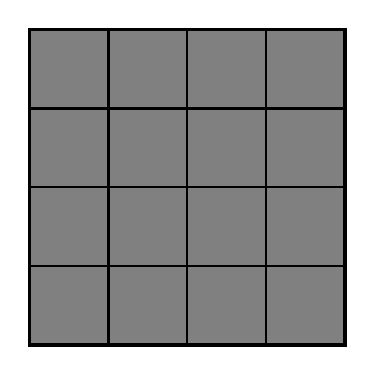
\begin{tikzpicture}
    \draw[draw=black,line width=0.5mm] (0,0) rectangle ++(4,4);
    \draw[draw=black,line width=0.3mm,fill=gray] (0,0) rectangle ++(1,1);
    \draw[draw=black,line width=0.3mm,fill=gray] (1,0) rectangle ++(1,1);
    \draw[draw=black,line width=0.3mm,fill=gray] (2,0) rectangle ++(1,1);
    \draw[draw=black,line width=0.3mm,fill=gray] (3,0) rectangle ++(1,1);
    \draw[draw=black,line width=0.3mm,fill=gray] (0,1) rectangle ++(1,1);
    \draw[draw=black,line width=0.3mm,fill=gray] (1,1) rectangle ++(1,1);
    \draw[draw=black,line width=0.3mm,fill=gray] (2,1) rectangle ++(1,1);
    \draw[draw=black,line width=0.3mm,fill=gray] (3,1) rectangle ++(1,1);
    \draw[draw=black,line width=0.3mm,fill=gray] (0,2) rectangle ++(1,1);
    \draw[draw=black,line width=0.3mm,fill=gray] (1,2) rectangle ++(1,1);
    \draw[draw=black,line width=0.3mm,fill=gray] (2,2) rectangle ++(1,1);
    \draw[draw=black,line width=0.3mm,fill=gray] (3,2) rectangle ++(1,1);
    \draw[draw=black,line width=0.3mm,fill=gray] (0,3) rectangle ++(1,1);
    \draw[draw=black,line width=0.3mm,fill=gray] (1,3) rectangle ++(1,1);
    \draw[draw=black,line width=0.3mm,fill=gray] (2,3) rectangle ++(1,1);
    \draw[draw=black,line width=0.3mm,fill=gray] (3,3) rectangle ++(1,1);
\end{tikzpicture}
}
        \caption{A 2D image with $4 \times 4$ pixels.}
    \end{subfigure} \hfill%
    \begin{subfigure}[b]{0.29\textwidth}
        \centering
        \captionsetup{justification=centering}
        \scalebox{1}{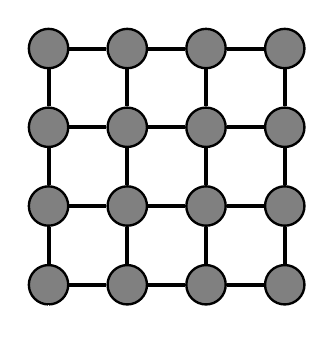
\begin{tikzpicture}
    \coordinate (origin) at (0,0);

    \node  (0) at (0,0.5) [draw,circle,line width=0.3mm,minimum width=0.5cm,fill=gray] {};
    \node  (1) at (1,0.5) [draw,circle,line width=0.3mm,minimum width=0.5cm,fill=gray] {};
    \node  (2) at (2,0.5) [draw,circle,line width=0.3mm,minimum width=0.5cm,fill=gray] {};
    \node  (3) at (3,0.5) [draw,circle,line width=0.3mm,minimum width=0.5cm,fill=gray] {};
    \node  (4) at (0,1.5) [draw,circle,line width=0.3mm,minimum width=0.5cm,fill=gray] {};
    \node  (5) at (1,1.5) [draw,circle,line width=0.3mm,minimum width=0.5cm,fill=gray] {};
    \node  (6) at (2,1.5) [draw,circle,line width=0.3mm,minimum width=0.5cm,fill=gray] {};
    \node  (7) at (3,1.5) [draw,circle,line width=0.3mm,minimum width=0.5cm,fill=gray] {};
    \node  (8) at (0,2.5) [draw,circle,line width=0.3mm,minimum width=0.5cm,fill=gray] {};
    \node  (9) at (1,2.5) [draw,circle,line width=0.3mm,minimum width=0.5cm,fill=gray] {};
    \node (10) at (2,2.5) [draw,circle,line width=0.3mm,minimum width=0.5cm,fill=gray] {};
    \node (11) at (3,2.5) [draw,circle,line width=0.3mm,minimum width=0.5cm,fill=gray] {};
    \node (12) at (0,3.5) [draw,circle,line width=0.3mm,minimum width=0.5cm,fill=gray] {};
    \node (13) at (1,3.5) [draw,circle,line width=0.3mm,minimum width=0.5cm,fill=gray] {};
    \node (14) at (2,3.5) [draw,circle,line width=0.3mm,minimum width=0.5cm,fill=gray] {};
    \node (15) at (3,3.5) [draw,circle,line width=0.3mm,minimum width=0.5cm,fill=gray] {};

    \draw[-,>=stealth,line width=0.5mm]  (0) to  (1);
    \draw[-,>=stealth,line width=0.5mm]  (1) to  (2);
    \draw[-,>=stealth,line width=0.5mm]  (2) to  (3);
    \draw[-,>=stealth,line width=0.5mm]  (4) to  (5);
    \draw[-,>=stealth,line width=0.5mm]  (5) to  (6);
    \draw[-,>=stealth,line width=0.5mm]  (6) to  (7);
    \draw[-,>=stealth,line width=0.5mm]  (8) to  (9);
    \draw[-,>=stealth,line width=0.5mm]  (9) to (10);
    \draw[-,>=stealth,line width=0.5mm] (10) to (11);
    \draw[-,>=stealth,line width=0.5mm] (12) to (13);
    \draw[-,>=stealth,line width=0.5mm] (13) to (14);
    \draw[-,>=stealth,line width=0.5mm] (14) to (15);

    \draw[-,>=stealth,line width=0.5mm]  (0) to  (4);
    \draw[-,>=stealth,line width=0.5mm]  (4) to  (8);
    \draw[-,>=stealth,line width=0.5mm]  (8) to  (12);
    \draw[-,>=stealth,line width=0.5mm]  (1) to  (5);
    \draw[-,>=stealth,line width=0.5mm]  (5) to  (9);
    \draw[-,>=stealth,line width=0.5mm]  (9) to  (13);
    \draw[-,>=stealth,line width=0.5mm]  (2) to  (6);
    \draw[-,>=stealth,line width=0.5mm]  (6) to (10);
    \draw[-,>=stealth,line width=0.5mm] (10) to (14);
    \draw[-,>=stealth,line width=0.5mm]  (3) to  (7);
    \draw[-,>=stealth,line width=0.5mm]  (7) to (11);
    \draw[-,>=stealth,line width=0.5mm] (11) to (15);

    \draw[-,>=stealth,line width=0mm,color=white] (origin) to (0);

\end{tikzpicture}
}
        \caption{A 4-connected pixel adjacency graph.}
    \end{subfigure} \hfill%
    \begin{subfigure}[b]{0.29\textwidth}
        \centering
        \captionsetup{justification=centering}
        \scalebox{1}{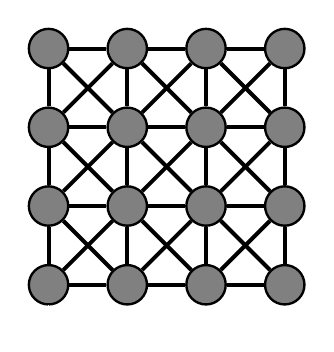
\begin{tikzpicture}
    \coordinate (origin) at (0,0);

    \node  (0) at (0,0.5) [draw,circle,line width=0.3mm,minimum width=0.5cm,fill=gray] {};
    \node  (1) at (1,0.5) [draw,circle,line width=0.3mm,minimum width=0.5cm,fill=gray] {};
    \node  (2) at (2,0.5) [draw,circle,line width=0.3mm,minimum width=0.5cm,fill=gray] {};
    \node  (3) at (3,0.5) [draw,circle,line width=0.3mm,minimum width=0.5cm,fill=gray] {};
    \node  (4) at (0,1.5) [draw,circle,line width=0.3mm,minimum width=0.5cm,fill=gray] {};
    \node  (5) at (1,1.5) [draw,circle,line width=0.3mm,minimum width=0.5cm,fill=gray] {};
    \node  (6) at (2,1.5) [draw,circle,line width=0.3mm,minimum width=0.5cm,fill=gray] {};
    \node  (7) at (3,1.5) [draw,circle,line width=0.3mm,minimum width=0.5cm,fill=gray] {};
    \node  (8) at (0,2.5) [draw,circle,line width=0.3mm,minimum width=0.5cm,fill=gray] {};
    \node  (9) at (1,2.5) [draw,circle,line width=0.3mm,minimum width=0.5cm,fill=gray] {};
    \node (10) at (2,2.5) [draw,circle,line width=0.3mm,minimum width=0.5cm,fill=gray] {};
    \node (11) at (3,2.5) [draw,circle,line width=0.3mm,minimum width=0.5cm,fill=gray] {};
    \node (12) at (0,3.5) [draw,circle,line width=0.3mm,minimum width=0.5cm,fill=gray] {};
    \node (13) at (1,3.5) [draw,circle,line width=0.3mm,minimum width=0.5cm,fill=gray] {};
    \node (14) at (2,3.5) [draw,circle,line width=0.3mm,minimum width=0.5cm,fill=gray] {};
    \node (15) at (3,3.5) [draw,circle,line width=0.3mm,minimum width=0.5cm,fill=gray] {};

    \draw[-,>=stealth,line width=0.5mm]  (0) to  (1);
    \draw[-,>=stealth,line width=0.5mm]  (1) to  (2);
    \draw[-,>=stealth,line width=0.5mm]  (2) to  (3);
    \draw[-,>=stealth,line width=0.5mm]  (4) to  (5);
    \draw[-,>=stealth,line width=0.5mm]  (5) to  (6);
    \draw[-,>=stealth,line width=0.5mm]  (6) to  (7);
    \draw[-,>=stealth,line width=0.5mm]  (8) to  (9);
    \draw[-,>=stealth,line width=0.5mm]  (9) to (10);
    \draw[-,>=stealth,line width=0.5mm] (10) to (11);
    \draw[-,>=stealth,line width=0.5mm] (12) to (13);
    \draw[-,>=stealth,line width=0.5mm] (13) to (14);
    \draw[-,>=stealth,line width=0.5mm] (14) to (15);

    \draw[-,>=stealth,line width=0.5mm]  (0) to  (4);
    \draw[-,>=stealth,line width=0.5mm]  (4) to  (8);
    \draw[-,>=stealth,line width=0.5mm]  (8) to  (12);
    \draw[-,>=stealth,line width=0.5mm]  (1) to  (5);
    \draw[-,>=stealth,line width=0.5mm]  (5) to  (9);
    \draw[-,>=stealth,line width=0.5mm]  (9) to  (13);
    \draw[-,>=stealth,line width=0.5mm]  (2) to  (6);
    \draw[-,>=stealth,line width=0.5mm]  (6) to (10);
    \draw[-,>=stealth,line width=0.5mm] (10) to (14);
    \draw[-,>=stealth,line width=0.5mm]  (3) to  (7);
    \draw[-,>=stealth,line width=0.5mm]  (7) to (11);
    \draw[-,>=stealth,line width=0.5mm] (11) to (15);

    \draw[-,>=stealth,line width=0.5mm]  (0) to  (5);
    \draw[-,>=stealth,line width=0.5mm]  (1) to  (6);
    \draw[-,>=stealth,line width=0.5mm]  (2) to  (7);
    \draw[-,>=stealth,line width=0.5mm]  (4) to (9);
    \draw[-,>=stealth,line width=0.5mm]  (5) to (10);
    \draw[-,>=stealth,line width=0.5mm]  (6) to (11);
    \draw[-,>=stealth,line width=0.5mm]  (8) to (13);
    \draw[-,>=stealth,line width=0.5mm]  (9) to (14);
    \draw[-,>=stealth,line width=0.5mm] (10) to (15);

    \draw[-,>=stealth,line width=0.5mm]  (1) to  (4);
    \draw[-,>=stealth,line width=0.5mm]  (2) to  (5);
    \draw[-,>=stealth,line width=0.5mm]  (3) to  (6);
    \draw[-,>=stealth,line width=0.5mm]  (5) to  (8);
    \draw[-,>=stealth,line width=0.5mm]  (6) to  (9);
    \draw[-,>=stealth,line width=0.5mm]  (7) to (10);
    \draw[-,>=stealth,line width=0.5mm]  (9) to (12);
    \draw[-,>=stealth,line width=0.5mm] (10) to (13);
    \draw[-,>=stealth,line width=0.5mm] (11) to (14);

    \draw[-,>=stealth,line width=0mm,color=white] (origin) to (0);

\end{tikzpicture}
}
        \caption{An 8-connected pixel adjacency graph.}
    \end{subfigure}%
    \caption[Pixel Adjacency Graphs]{Pixel adjacency graphs.}
    \label{fig:pixelAdjacency}
\end{figure}
\begin{figure}[h!]
    \centering
    \begin{subfigure}[b]{0.29\textwidth}
        \centering
        \captionsetup{justification=centering}
        \scalebox{1}{\begin{tikzpicture}
    \draw[draw=black,line width=0.5mm] (0,0) rectangle ++(3,3);
    \draw[draw=black,line width=0.3mm,fill=homomorphicGreen] (0,0) rectangle ++(1,1);
    \draw[draw=black,line width=0.3mm,fill=homomorphicGreen] (1,0) rectangle ++(1,1);
    \draw[draw=black,line width=0.3mm,fill=homomorphicGreen] (2,0) rectangle ++(1,1);
    \draw[draw=black,line width=0.3mm,fill=homomorphicGreen] (0,1) rectangle ++(1,1);
    \draw[draw=black,line width=0.3mm,fill=homomorphicGreen] (1,1) rectangle ++(1,1);
    \draw[draw=black,line width=0.3mm,fill=homomorphicGreen] (2,1) rectangle ++(1,1);
    \draw[draw=black,line width=0.3mm,fill=homomorphicGreen] (0,2) rectangle ++(1,1);
    \draw[draw=black,line width=0.3mm,fill=homomorphicGreen] (1,2) rectangle ++(1,1);
    \draw[draw=black,line width=0.3mm,fill=homomorphicGreen] (2,2) rectangle ++(1,1);
    

    \draw[draw=black,line width=0.5mm] (-0.5,-0.5) rectangle ++(3,3);
    \draw[draw=black,line width=0.3mm,fill=ckksRed] (-0.5,-0.5) rectangle ++(1,1);
    \draw[draw=black,line width=0.3mm,fill=ckksRed]  (0.5,-0.5) rectangle ++(1,1);
    \draw[draw=black,line width=0.3mm,fill=ckksRed]  (1.5,-0.5) rectangle ++(1,1);
    \draw[draw=black,line width=0.3mm,fill=ckksRed] (-0.5, 0.5) rectangle ++(1,1);
    \draw[draw=black,line width=0.3mm,fill=ckksRed]  (0.5, 0.5) rectangle ++(1,1);
    \draw[draw=black,line width=0.3mm,fill=ckksRed]  (1.5, 0.5) rectangle ++(1,1);
    \draw[draw=black,line width=0.3mm,fill=ckksRed] (-0.5, 1.5) rectangle ++(1,1);
    \draw[draw=black,line width=0.3mm,fill=ckksRed]  (0.5, 1.5) rectangle ++(1,1);
    \draw[draw=black,line width=0.3mm,fill=ckksRed]  (1.5, 1.5) rectangle ++(1,1);

    \draw[draw=black,line width=0.5mm] (-1,-1) rectangle ++(3,3);
    \draw[draw=black,line width=0.3mm,fill=mekksBlue] (-1,-1) rectangle ++(1,1);
    \draw[draw=black,line width=0.3mm,fill=mekksBlue]  (0,-1) rectangle ++(1,1);
    \draw[draw=black,line width=0.3mm,fill=mekksBlue]  (1,-1) rectangle ++(1,1);
    \draw[draw=black,line width=0.3mm,fill=mekksBlue] (-1, 0) rectangle ++(1,1);
    \draw[draw=black,line width=0.3mm,fill=mekksBlue]  (0, 0) rectangle ++(1,1);
    \draw[draw=black,line width=0.3mm,fill=mekksBlue]  (1, 0) rectangle ++(1,1);
    \draw[draw=black,line width=0.3mm,fill=mekksBlue] (-1, 1) rectangle ++(1,1);
    \draw[draw=black,line width=0.3mm,fill=mekksBlue]  (0, 1) rectangle ++(1,1);
    \draw[draw=black,line width=0.3mm,fill=mekksBlue]  (1, 1) rectangle ++(1,1);
\end{tikzpicture}
}
        \caption{A video with three frames of $3 \times 3$ pixels.}
    \end{subfigure} \hfill%
    \begin{subfigure}[b]{0.29\textwidth}
        \centering
        \captionsetup{justification=centering}
        \scalebox{0.5}{\begin{tikzpicture}
    \node  (0g) at (1,0,-2.5) [draw,circle,line width=0.3mm,minimum width=0.5cm,fill=lightgray] {};
    \node  (1g) at (4,0,-2.5) [draw,circle,line width=0.3mm,minimum width=0.5cm,fill=lightgray] {};
    \node  (2g) at (7,0,-2.5) [draw,circle,line width=0.3mm,minimum width=0.5cm,fill=lightgray] {};
    \node  (3g) at (1,3,-2.5) [draw,circle,line width=0.3mm,minimum width=0.5cm,fill=lightgray] {};
    \node  (4g) at (4,3,-2.5) [draw,circle,line width=0.3mm,minimum width=0.5cm,fill=homomorphicGreen] {};
    \node  (5g) at (7,3,-2.5) [draw,circle,line width=0.3mm,minimum width=0.5cm,fill=lightgray] {};
    \node  (6g) at (1,6,-2.5) [draw,circle,line width=0.3mm,minimum width=0.5cm,fill=lightgray] {};
    \node  (7g) at (4,6,-2.5) [draw,circle,line width=0.3mm,minimum width=0.5cm,fill=lightgray] {};
    \node  (8g) at (7,6,-2.5) [draw,circle,line width=0.3mm,minimum width=0.5cm,fill=lightgray] {};



    \node  (0r) at (1,0,0) [draw,circle,line width=0.3mm,minimum width=0.5cm,fill=lightgray] {};
    \node  (1r) at (4,0,0) [draw,circle,line width=0.3mm,minimum width=0.5cm,fill=ckksRed] {};
    \node  (2r) at (7,0,0) [draw,circle,line width=0.3mm,minimum width=0.5cm,fill=lightgray] {};
    \node  (3r) at (1,3,0) [draw,circle,line width=0.3mm,minimum width=0.5cm,fill=ckksRed] {};
    \node  (4r) at (4,3,0) [draw,circle,line width=0.3mm,minimum width=0.5cm,fill=ckksRed] {};
    \node  (5r) at (7,3,0) [draw,circle,line width=0.3mm,minimum width=0.5cm,fill=ckksRed] {};
    \node  (6r) at (1,6,0) [draw,circle,line width=0.3mm,minimum width=0.5cm,fill=lightgray] {};
    \node  (7r) at (4,6,0) [draw,circle,line width=0.3mm,minimum width=0.5cm,fill=ckksRed] {};
    \node  (8r) at (7,6,0) [draw,circle,line width=0.3mm,minimum width=0.5cm,fill=lightgray] {};



    \node  (0b) at (1,0,2.5) [draw,circle,line width=0.3mm,minimum width=0.5cm,fill=lightgray] {};
    \node  (1b) at (4,0,2.5) [draw,circle,line width=0.3mm,minimum width=0.5cm,fill=lightgray] {};
    \node  (2b) at (7,0,2.5) [draw,circle,line width=0.3mm,minimum width=0.5cm,fill=lightgray] {};
    \node  (3b) at (1,3,2.5) [draw,circle,line width=0.3mm,minimum width=0.5cm,fill=lightgray] {};
    \node  (4b) at (4,3,2.5) [draw,circle,line width=0.3mm,minimum width=0.5cm,fill=mekksBlue] {};
    \node  (5b) at (7,3,2.5) [draw,circle,line width=0.3mm,minimum width=0.5cm,fill=lightgray] {};
    \node  (6b) at (1,6,2.5) [draw,circle,line width=0.3mm,minimum width=0.5cm,fill=lightgray] {};
    \node  (7b) at (4,6,2.5) [draw,circle,line width=0.3mm,minimum width=0.5cm,fill=lightgray] {};
    \node  (8b) at (7,6,2.5) [draw,circle,line width=0.3mm,minimum width=0.5cm,fill=lightgray] {};



    \draw[-,>=stealth,line width=0.5mm]  (4r) to  (1r);
    \draw[-,>=stealth,line width=0.5mm]  (4r) to  (3r);
    \draw[-,>=stealth,line width=0.5mm]  (4r) to  (5r);
    \draw[-,>=stealth,line width=0.5mm]  (4r) to  (7r);
    \draw[-,>=stealth,line width=0.5mm]  (4r) to  (4b);
    \draw[-,>=stealth,line width=0.5mm]  (4r) to  (4g);



    \draw[-,>=stealth,line width=0.5mm,dashed]  (0g) to  (1g);
    \draw[-,>=stealth,line width=0.5mm,dashed]  (1g) to  (2g);
    \draw[-,>=stealth,line width=0.5mm,dashed]  (3g) to  (4g);
    \draw[-,>=stealth,line width=0.5mm,dashed]  (4g) to  (5g);
    \draw[-,>=stealth,line width=0.5mm,dashed]  (6g) to  (7g);
    \draw[-,>=stealth,line width=0.5mm,dashed]  (7g) to  (8g);
    \draw[-,>=stealth,line width=0.5mm,dashed]  (0g) to  (3g);
    \draw[-,>=stealth,line width=0.5mm,dashed]  (1g) to  (4g);
    \draw[-,>=stealth,line width=0.5mm,dashed]  (2g) to  (5g);
    \draw[-,>=stealth,line width=0.5mm,dashed]  (3g) to  (6g);
    \draw[-,>=stealth,line width=0.5mm,dashed]  (4g) to  (7g);
    \draw[-,>=stealth,line width=0.5mm,dashed]  (5g) to  (8g);
    \draw[-,>=stealth,line width=0.5mm,dashed]  (0r) to  (1r);
    \draw[-,>=stealth,line width=0.5mm,dashed]  (1r) to  (2r);
    \draw[-,>=stealth,line width=0.5mm,dashed]  (3r) to  (4r);
    \draw[-,>=stealth,line width=0.5mm,dashed]  (4r) to  (5r);
    \draw[-,>=stealth,line width=0.5mm,dashed]  (6r) to  (7r);
    \draw[-,>=stealth,line width=0.5mm,dashed]  (7r) to  (8r);
    \draw[-,>=stealth,line width=0.5mm,dashed]  (0r) to  (3r);
    \draw[-,>=stealth,line width=0.5mm,dashed]  (1r) to  (4r);
    \draw[-,>=stealth,line width=0.5mm,dashed]  (2r) to  (5r);
    \draw[-,>=stealth,line width=0.5mm,dashed]  (3r) to  (6r);
    \draw[-,>=stealth,line width=0.5mm,dashed]  (4r) to  (7r);
    \draw[-,>=stealth,line width=0.5mm,dashed]  (5r) to  (8r);
    \draw[-,>=stealth,line width=0.5mm,dashed]  (0b) to  (1b);
    \draw[-,>=stealth,line width=0.5mm,dashed]  (1b) to  (2b);
    \draw[-,>=stealth,line width=0.5mm,dashed]  (3b) to  (4b);
    \draw[-,>=stealth,line width=0.5mm,dashed]  (4b) to  (5b);
    \draw[-,>=stealth,line width=0.5mm,dashed]  (6b) to  (7b);
    \draw[-,>=stealth,line width=0.5mm,dashed]  (7b) to  (8b);
    \draw[-,>=stealth,line width=0.5mm,dashed]  (0b) to  (3b);
    \draw[-,>=stealth,line width=0.5mm,dashed]  (1b) to  (4b);
    \draw[-,>=stealth,line width=0.5mm,dashed]  (2b) to  (5b);
    \draw[-,>=stealth,line width=0.5mm,dashed]  (3b) to  (6b);
    \draw[-,>=stealth,line width=0.5mm,dashed]  (4b) to  (7b);
    \draw[-,>=stealth,line width=0.5mm,dashed]  (5b) to  (8b);
    \draw[-,>=stealth,line width=0.5mm,dashed]  (0b) to  (0r);
    \draw[-,>=stealth,line width=0.5mm,dashed]  (1b) to  (1r);
    \draw[-,>=stealth,line width=0.5mm,dashed]  (2b) to  (2r);
    \draw[-,>=stealth,line width=0.5mm,dashed]  (3b) to  (3r);
    \draw[-,>=stealth,line width=0.5mm,dashed]  (4b) to  (4r);
    \draw[-,>=stealth,line width=0.5mm,dashed]  (5b) to  (5r);
    \draw[-,>=stealth,line width=0.5mm,dashed]  (6b) to  (6r);
    \draw[-,>=stealth,line width=0.5mm,dashed]  (7b) to  (7r);
    \draw[-,>=stealth,line width=0.5mm,dashed]  (8b) to  (8r);
    \draw[-,>=stealth,line width=0.5mm,dashed]  (0g) to  (0r);
    \draw[-,>=stealth,line width=0.5mm,dashed]  (1g) to  (1r);
    \draw[-,>=stealth,line width=0.5mm,dashed]  (2g) to  (2r);
    \draw[-,>=stealth,line width=0.5mm,dashed]  (3g) to  (3r);
    \draw[-,>=stealth,line width=0.5mm,dashed]  (4g) to  (4r);
    \draw[-,>=stealth,line width=0.5mm,dashed]  (5g) to  (5r);
    \draw[-,>=stealth,line width=0.5mm,dashed]  (6g) to  (6r);
    \draw[-,>=stealth,line width=0.5mm,dashed]  (7g) to  (7r);
    \draw[-,>=stealth,line width=0.5mm,dashed]  (8g) to  (8r);
\end{tikzpicture}
}
        \caption{A 6-connected 3D pixel adjacency graph.}
    \end{subfigure} \hfill%
    \begin{subfigure}[b]{0.29\textwidth}
        \centering
        \captionsetup{justification=centering}
        \scalebox{0.5}{\begin{tikzpicture}
    \node  (0g) at (1,0,-2.5) [draw,circle,line width=0.3mm,minimum width=0.5cm,fill=lightgray] {};
    \node  (1g) at (4,0,-2.5) [draw,circle,line width=0.3mm,minimum width=0.5cm,fill=homomorphicGreen] {};
    \node  (2g) at (7,0,-2.5) [draw,circle,line width=0.3mm,minimum width=0.5cm,fill=lightgray] {};
    \node  (3g) at (1,3,-2.5) [draw,circle,line width=0.3mm,minimum width=0.5cm,fill=homomorphicGreen] {};
    \node  (4g) at (4,3,-2.5) [draw,circle,line width=0.3mm,minimum width=0.5cm,fill=homomorphicGreen] {};
    \node  (5g) at (7,3,-2.5) [draw,circle,line width=0.3mm,minimum width=0.5cm,fill=homomorphicGreen] {};
    \node  (6g) at (1,6,-2.5) [draw,circle,line width=0.3mm,minimum width=0.5cm,fill=lightgray] {};
    \node  (7g) at (4,6,-2.5) [draw,circle,line width=0.3mm,minimum width=0.5cm,fill=homomorphicGreen] {};
    \node  (8g) at (7,6,-2.5) [draw,circle,line width=0.3mm,minimum width=0.5cm,fill=lightgray] {};



    \node  (0r) at (1,0,0) [draw,circle,line width=0.3mm,minimum width=0.5cm,fill=ckksRed] {};
    \node  (1r) at (4,0,0) [draw,circle,line width=0.3mm,minimum width=0.5cm,fill=ckksRed] {};
    \node  (2r) at (7,0,0) [draw,circle,line width=0.3mm,minimum width=0.5cm,fill=ckksRed] {};
    \node  (3r) at (1,3,0) [draw,circle,line width=0.3mm,minimum width=0.5cm,fill=ckksRed] {};
    \node  (4r) at (4,3,0) [draw,circle,line width=0.3mm,minimum width=0.5cm,fill=ckksRed] {};
    \node  (5r) at (7,3,0) [draw,circle,line width=0.3mm,minimum width=0.5cm,fill=ckksRed] {};
    \node  (6r) at (1,6,0) [draw,circle,line width=0.3mm,minimum width=0.5cm,fill=ckksRed] {};
    \node  (7r) at (4,6,0) [draw,circle,line width=0.3mm,minimum width=0.5cm,fill=ckksRed] {};
    \node  (8r) at (7,6,0) [draw,circle,line width=0.3mm,minimum width=0.5cm,fill=ckksRed] {};


    \draw[-,>=stealth,line width=0.5mm]  (4r) to  (0r);
    \draw[-,>=stealth,line width=0.5mm]  (4r) to  (1r);
    \draw[-,>=stealth,line width=0.5mm]  (4r) to  (2r);
    \draw[-,>=stealth,line width=0.5mm]  (4r) to  (3r);
    \draw[-,>=stealth,line width=0.5mm]  (4r) to  (5r);
    \draw[-,>=stealth,line width=0.5mm]  (4r) to  (6r);
    \draw[-,>=stealth,line width=0.5mm]  (4r) to  (7r);
    \draw[-,>=stealth,line width=0.5mm]  (4r) to  (8r);



    \node  (0b) at (1,0,2.5) [draw,circle,line width=0.3mm,minimum width=0.5cm,fill=lightgray] {};
    \node  (1b) at (4,0,2.5) [draw,circle,line width=0.3mm,minimum width=0.5cm,fill=mekksBlue] {};
    \node  (2b) at (7,0,2.5) [draw,circle,line width=0.3mm,minimum width=0.5cm,fill=lightgray] {};
    \node  (3b) at (1,3,2.5) [draw,circle,line width=0.3mm,minimum width=0.5cm,fill=mekksBlue] {};
    \node  (4b) at (4,3,2.5) [draw,circle,line width=0.3mm,minimum width=0.5cm,fill=mekksBlue] {};
    \node  (5b) at (7,3,2.5) [draw,circle,line width=0.3mm,minimum width=0.5cm,fill=mekksBlue] {};
    \node  (6b) at (1,6,2.5) [draw,circle,line width=0.3mm,minimum width=0.5cm,fill=lightgray] {};
    \node  (7b) at (4,6,2.5) [draw,circle,line width=0.3mm,minimum width=0.5cm,fill=mekksBlue] {};
    \node  (8b) at (7,6,2.5) [draw,circle,line width=0.3mm,minimum width=0.5cm,fill=lightgray] {};



    
    \draw[-,>=stealth,line width=0.5mm]  (4r) to  (1b);
    \draw[-,>=stealth,line width=0.5mm]  (4r) to  (3b);
    \draw[-,>=stealth,line width=0.5mm]  (4r) to  (4b);
    \draw[-,>=stealth,line width=0.5mm]  (4r) to  (5b);
    \draw[-,>=stealth,line width=0.5mm]  (4r) to  (7b);
    \draw[-,>=stealth,line width=0.5mm]  (4r) to  (1g);
    \draw[-,>=stealth,line width=0.5mm]  (4r) to  (3g);
    \draw[-,>=stealth,line width=0.5mm]  (4r) to  (4g);
    \draw[-,>=stealth,line width=0.5mm]  (4r) to  (5g);
    \draw[-,>=stealth,line width=0.5mm]  (4r) to  (7g);



    \draw[-,>=stealth,line width=0.5mm,dashed]  (0g) to  (1g);
    \draw[-,>=stealth,line width=0.5mm,dashed]  (1g) to  (2g);
    \draw[-,>=stealth,line width=0.5mm,dashed]  (3g) to  (4g);
    \draw[-,>=stealth,line width=0.5mm,dashed]  (4g) to  (5g);
    \draw[-,>=stealth,line width=0.5mm,dashed]  (6g) to  (7g);
    \draw[-,>=stealth,line width=0.5mm,dashed]  (7g) to  (8g);
    \draw[-,>=stealth,line width=0.5mm,dashed]  (0g) to  (3g);
    \draw[-,>=stealth,line width=0.5mm,dashed]  (1g) to  (4g);
    \draw[-,>=stealth,line width=0.5mm,dashed]  (2g) to  (5g);
    \draw[-,>=stealth,line width=0.5mm,dashed]  (3g) to  (6g);
    \draw[-,>=stealth,line width=0.5mm,dashed]  (4g) to  (7g);
    \draw[-,>=stealth,line width=0.5mm,dashed]  (5g) to  (8g);
    \draw[-,>=stealth,line width=0.5mm,dashed]  (0r) to  (1r);
    \draw[-,>=stealth,line width=0.5mm,dashed]  (1r) to  (2r);
    \draw[-,>=stealth,line width=0.5mm,dashed]  (3r) to  (4r);
    \draw[-,>=stealth,line width=0.5mm,dashed]  (4r) to  (5r);
    \draw[-,>=stealth,line width=0.5mm,dashed]  (6r) to  (7r);
    \draw[-,>=stealth,line width=0.5mm,dashed]  (7r) to  (8r);
    \draw[-,>=stealth,line width=0.5mm,dashed]  (0r) to  (3r);
    \draw[-,>=stealth,line width=0.5mm,dashed]  (1r) to  (4r);
    \draw[-,>=stealth,line width=0.5mm,dashed]  (2r) to  (5r);
    \draw[-,>=stealth,line width=0.5mm,dashed]  (3r) to  (6r);
    \draw[-,>=stealth,line width=0.5mm,dashed]  (4r) to  (7r);
    \draw[-,>=stealth,line width=0.5mm,dashed]  (5r) to  (8r);
    \draw[-,>=stealth,line width=0.5mm,dashed]  (0b) to  (1b);
    \draw[-,>=stealth,line width=0.5mm,dashed]  (1b) to  (2b);
    \draw[-,>=stealth,line width=0.5mm,dashed]  (3b) to  (4b);
    \draw[-,>=stealth,line width=0.5mm,dashed]  (4b) to  (5b);
    \draw[-,>=stealth,line width=0.5mm,dashed]  (6b) to  (7b);
    \draw[-,>=stealth,line width=0.5mm,dashed]  (7b) to  (8b);
    \draw[-,>=stealth,line width=0.5mm,dashed]  (0b) to  (3b);
    \draw[-,>=stealth,line width=0.5mm,dashed]  (1b) to  (4b);
    \draw[-,>=stealth,line width=0.5mm,dashed]  (2b) to  (5b);
    \draw[-,>=stealth,line width=0.5mm,dashed]  (3b) to  (6b);
    \draw[-,>=stealth,line width=0.5mm,dashed]  (4b) to  (7b);
    \draw[-,>=stealth,line width=0.5mm,dashed]  (5b) to  (8b);
    \draw[-,>=stealth,line width=0.5mm,dashed]  (0b) to  (0r);
    \draw[-,>=stealth,line width=0.5mm,dashed]  (1b) to  (1r);
    \draw[-,>=stealth,line width=0.5mm,dashed]  (2b) to  (2r);
    \draw[-,>=stealth,line width=0.5mm,dashed]  (3b) to  (3r);
    \draw[-,>=stealth,line width=0.5mm,dashed]  (4b) to  (4r);
    \draw[-,>=stealth,line width=0.5mm,dashed]  (5b) to  (5r);
    \draw[-,>=stealth,line width=0.5mm,dashed]  (6b) to  (6r);
    \draw[-,>=stealth,line width=0.5mm,dashed]  (7b) to  (7r);
    \draw[-,>=stealth,line width=0.5mm,dashed]  (8b) to  (8r);
    \draw[-,>=stealth,line width=0.5mm,dashed]  (0g) to  (0r);
    \draw[-,>=stealth,line width=0.5mm,dashed]  (1g) to  (1r);
    \draw[-,>=stealth,line width=0.5mm,dashed]  (2g) to  (2r);
    \draw[-,>=stealth,line width=0.5mm,dashed]  (3g) to  (3r);
    \draw[-,>=stealth,line width=0.5mm,dashed]  (4g) to  (4r);
    \draw[-,>=stealth,line width=0.5mm,dashed]  (5g) to  (5r);
    \draw[-,>=stealth,line width=0.5mm,dashed]  (6g) to  (6r);
    \draw[-,>=stealth,line width=0.5mm,dashed]  (7g) to  (7r);
    \draw[-,>=stealth,line width=0.5mm,dashed]  (8g) to  (8r);
\end{tikzpicture}
}
        \caption{An 18-connected 3D pixel adjacency graph.}
    \end{subfigure}%
    \caption[3D Pixel Adjacency Graphs]{3D pixel adjacency graphs.}
    \label{fig:3dAdjacency}
\end{figure}
\smallskip \\ \indent
The pixel adjacency graphs can na\"ively be applied to any image by creating a node for each pixel and an edge for every adjacency. While this does provide some opportunity for optimisations in regards to inference algorithms, it is unlikely to reduce the \textit{video size}, so it will have little positive impact on \textit{transmission time}.
\smallskip \\ \indent
However, all hope is not lost. Improvements can be made to this representation to reduce the overall size of each frame in the video. Primarily, the pixel adjacency graph can be extended to become \textit{region adjacency graphs}. In this case, rather than representing each individual pixel with a node, similar regions of an image are amalgamated into a single node, reducing the number of elements that need to be transmitted. Figure \ref{fig:pixelToRegion} provides a pictorial example of this.
\begin{figure}[htp]
    \centering
    \begin{subfigure}[b]{0.45\textwidth}
        \centering
        \captionsetup{justification=centering}
        \scalebox{0.5}{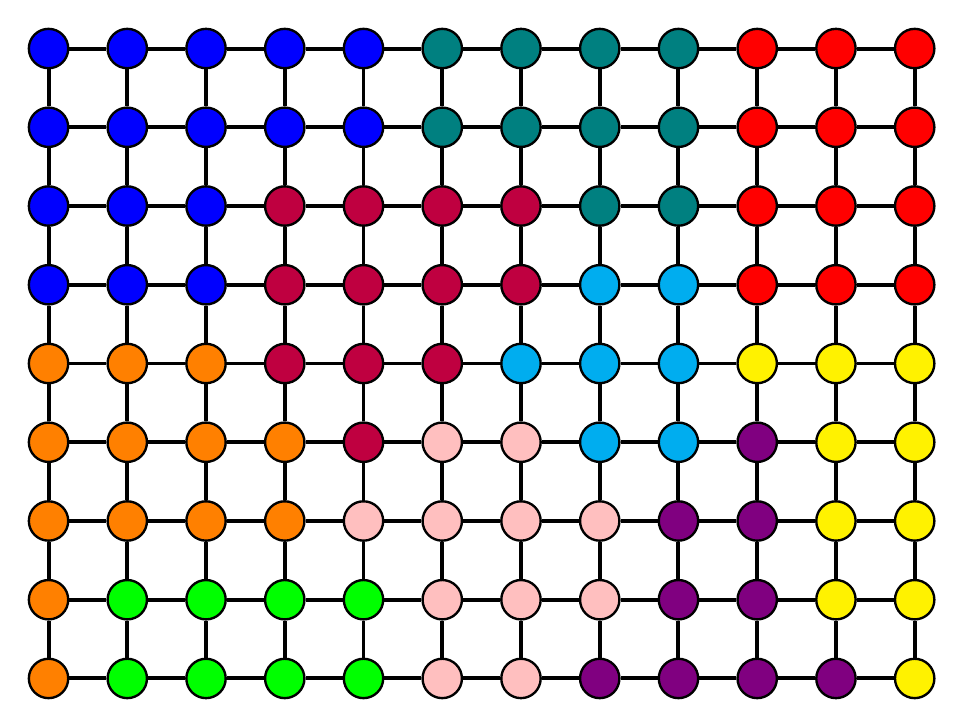
\begin{tikzpicture}
    \node (aa) at  (0,0) [draw,circle,line width=0.3mm,minimum width=0.5cm,fill=orange] {};
    \node (ba) at  (1,0) [draw,circle,line width=0.3mm,minimum width=0.5cm,fill=green] {};
    \node (ca) at  (2,0) [draw,circle,line width=0.3mm,minimum width=0.5cm,fill=green] {};
    \node (da) at  (3,0) [draw,circle,line width=0.3mm,minimum width=0.5cm,fill=green] {};
    \node (ea) at  (4,0) [draw,circle,line width=0.3mm,minimum width=0.5cm,fill=green] {};
    \node (fa) at  (5,0) [draw,circle,line width=0.3mm,minimum width=0.5cm,fill=pink] {};
    \node (ga) at  (6,0) [draw,circle,line width=0.3mm,minimum width=0.5cm,fill=pink] {};
    \node (ha) at  (7,0) [draw,circle,line width=0.3mm,minimum width=0.5cm,fill=violet] {};
    \node (ia) at  (8,0) [draw,circle,line width=0.3mm,minimum width=0.5cm,fill=violet] {};
    \node (ja) at  (9,0) [draw,circle,line width=0.3mm,minimum width=0.5cm,fill=violet] {};
    \node (ka) at (10,0) [draw,circle,line width=0.3mm,minimum width=0.5cm,fill=violet] {};
    \node (la) at (11,0) [draw,circle,line width=0.3mm,minimum width=0.5cm,fill=yellow] {};    

    \node (ab) at  (0,1) [draw,circle,line width=0.3mm,minimum width=0.5cm,fill=orange] {};
    \node (bb) at  (1,1) [draw,circle,line width=0.3mm,minimum width=0.5cm,fill=green] {};
    \node (cb) at  (2,1) [draw,circle,line width=0.3mm,minimum width=0.5cm,fill=green] {};
    \node (db) at  (3,1) [draw,circle,line width=0.3mm,minimum width=0.5cm,fill=green] {};
    \node (eb) at  (4,1) [draw,circle,line width=0.3mm,minimum width=0.5cm,fill=green] {};
    \node (fb) at  (5,1) [draw,circle,line width=0.3mm,minimum width=0.5cm,fill=pink] {};
    \node (gb) at  (6,1) [draw,circle,line width=0.3mm,minimum width=0.5cm,fill=pink] {};
    \node (hb) at  (7,1) [draw,circle,line width=0.3mm,minimum width=0.5cm,fill=pink] {};
    \node (ib) at  (8,1) [draw,circle,line width=0.3mm,minimum width=0.5cm,fill=violet] {};
    \node (jb) at  (9,1) [draw,circle,line width=0.3mm,minimum width=0.5cm,fill=violet] {};
    \node (kb) at (10,1) [draw,circle,line width=0.3mm,minimum width=0.5cm,fill=yellow] {};
    \node (lb) at (11,1) [draw,circle,line width=0.3mm,minimum width=0.5cm,fill=yellow] {};    

    \node (ac) at  (0,2) [draw,circle,line width=0.3mm,minimum width=0.5cm,fill=orange] {};
    \node (bc) at  (1,2) [draw,circle,line width=0.3mm,minimum width=0.5cm,fill=orange] {};
    \node (cc) at  (2,2) [draw,circle,line width=0.3mm,minimum width=0.5cm,fill=orange] {};
    \node (dc) at  (3,2) [draw,circle,line width=0.3mm,minimum width=0.5cm,fill=orange] {};
    \node (ec) at  (4,2) [draw,circle,line width=0.3mm,minimum width=0.5cm,fill=pink] {};
    \node (fc) at  (5,2) [draw,circle,line width=0.3mm,minimum width=0.5cm,fill=pink] {};
    \node (gc) at  (6,2) [draw,circle,line width=0.3mm,minimum width=0.5cm,fill=pink] {};
    \node (hc) at  (7,2) [draw,circle,line width=0.3mm,minimum width=0.5cm,fill=pink] {};
    \node (ic) at  (8,2) [draw,circle,line width=0.3mm,minimum width=0.5cm,fill=violet] {};
    \node (jc) at  (9,2) [draw,circle,line width=0.3mm,minimum width=0.5cm,fill=violet] {};
    \node (kc) at (10,2) [draw,circle,line width=0.3mm,minimum width=0.5cm,fill=yellow] {};
    \node (lc) at (11,2) [draw,circle,line width=0.3mm,minimum width=0.5cm,fill=yellow] {};    

    \node (ad) at  (0,3) [draw,circle,line width=0.3mm,minimum width=0.5cm,fill=orange] {};
    \node (bd) at  (1,3) [draw,circle,line width=0.3mm,minimum width=0.5cm,fill=orange] {};
    \node (cd) at  (2,3) [draw,circle,line width=0.3mm,minimum width=0.5cm,fill=orange] {};
    \node (dd) at  (3,3) [draw,circle,line width=0.3mm,minimum width=0.5cm,fill=orange] {};
    \node (ed) at  (4,3) [draw,circle,line width=0.3mm,minimum width=0.5cm,fill=purple] {};
    \node (fd) at  (5,3) [draw,circle,line width=0.3mm,minimum width=0.5cm,fill=pink] {};
    \node (gd) at  (6,3) [draw,circle,line width=0.3mm,minimum width=0.5cm,fill=pink] {};
    \node (hd) at  (7,3) [draw,circle,line width=0.3mm,minimum width=0.5cm,fill=cyan] {};
    \node (id) at  (8,3) [draw,circle,line width=0.3mm,minimum width=0.5cm,fill=cyan] {};
    \node (jd) at  (9,3) [draw,circle,line width=0.3mm,minimum width=0.5cm,fill=violet] {};
    \node (kd) at (10,3) [draw,circle,line width=0.3mm,minimum width=0.5cm,fill=yellow] {};
    \node (ld) at (11,3) [draw,circle,line width=0.3mm,minimum width=0.5cm,fill=yellow] {};    

    \node (ae) at  (0,4) [draw,circle,line width=0.3mm,minimum width=0.5cm,fill=orange] {};
    \node (be) at  (1,4) [draw,circle,line width=0.3mm,minimum width=0.5cm,fill=orange] {};
    \node (ce) at  (2,4) [draw,circle,line width=0.3mm,minimum width=0.5cm,fill=orange] {};
    \node (de) at  (3,4) [draw,circle,line width=0.3mm,minimum width=0.5cm,fill=purple] {};
    \node (ee) at  (4,4) [draw,circle,line width=0.3mm,minimum width=0.5cm,fill=purple] {};
    \node (fe) at  (5,4) [draw,circle,line width=0.3mm,minimum width=0.5cm,fill=purple] {};
    \node (ge) at  (6,4) [draw,circle,line width=0.3mm,minimum width=0.5cm,fill=cyan] {};
    \node (he) at  (7,4) [draw,circle,line width=0.3mm,minimum width=0.5cm,fill=cyan] {};
    \node (ie) at  (8,4) [draw,circle,line width=0.3mm,minimum width=0.5cm,fill=cyan] {};
    \node (je) at  (9,4) [draw,circle,line width=0.3mm,minimum width=0.5cm,fill=yellow] {};
    \node (ke) at (10,4) [draw,circle,line width=0.3mm,minimum width=0.5cm,fill=yellow] {};
    \node (le) at (11,4) [draw,circle,line width=0.3mm,minimum width=0.5cm,fill=yellow] {};    

    \node (bf) at  (1,5) [draw,circle,line width=0.3mm,minimum width=0.5cm,fill=blue] {};
    \node (af) at  (0,5) [draw,circle,line width=0.3mm,minimum width=0.5cm,fill=blue] {};
    \node (cf) at  (2,5) [draw,circle,line width=0.3mm,minimum width=0.5cm,fill=blue] {};
    \node (df) at  (3,5) [draw,circle,line width=0.3mm,minimum width=0.5cm,fill=purple] {};
    \node (ef) at  (4,5) [draw,circle,line width=0.3mm,minimum width=0.5cm,fill=purple] {};
    \node (ff) at  (5,5) [draw,circle,line width=0.3mm,minimum width=0.5cm,fill=purple] {};
    \node (gf) at  (6,5) [draw,circle,line width=0.3mm,minimum width=0.5cm,fill=purple] {};
    \node (hf) at  (7,5) [draw,circle,line width=0.3mm,minimum width=0.5cm,fill=cyan] {};
    \node (if) at  (8,5) [draw,circle,line width=0.3mm,minimum width=0.5cm,fill=cyan] {};
    \node (jf) at  (9,5) [draw,circle,line width=0.3mm,minimum width=0.5cm,fill=red] {};
    \node (kf) at (10,5) [draw,circle,line width=0.3mm,minimum width=0.5cm,fill=red] {};
    \node (lf) at (11,5) [draw,circle,line width=0.3mm,minimum width=0.5cm,fill=red] {};    
    
    \node (ag) at  (0,6) [draw,circle,line width=0.3mm,minimum width=0.5cm,fill=blue] {};
    \node (bg) at  (1,6) [draw,circle,line width=0.3mm,minimum width=0.5cm,fill=blue] {};
    \node (cg) at  (2,6) [draw,circle,line width=0.3mm,minimum width=0.5cm,fill=blue] {};
    \node (dg) at  (3,6) [draw,circle,line width=0.3mm,minimum width=0.5cm,fill=purple] {};
    \node (eg) at  (4,6) [draw,circle,line width=0.3mm,minimum width=0.5cm,fill=purple] {};
    \node (fg) at  (5,6) [draw,circle,line width=0.3mm,minimum width=0.5cm,fill=purple] {};
    \node (gg) at  (6,6) [draw,circle,line width=0.3mm,minimum width=0.5cm,fill=purple] {};
    \node (hg) at  (7,6) [draw,circle,line width=0.3mm,minimum width=0.5cm,fill=teal] {};
    \node (ig) at  (8,6) [draw,circle,line width=0.3mm,minimum width=0.5cm,fill=teal] {};
    \node (jg) at  (9,6) [draw,circle,line width=0.3mm,minimum width=0.5cm,fill=red] {};
    \node (kg) at (10,6) [draw,circle,line width=0.3mm,minimum width=0.5cm,fill=red] {};
    \node (lg) at (11,6) [draw,circle,line width=0.3mm,minimum width=0.5cm,fill=red] {};    
    
    \node (ah) at  (0,7) [draw,circle,line width=0.3mm,minimum width=0.5cm,fill=blue] {};
    \node (bh) at  (1,7) [draw,circle,line width=0.3mm,minimum width=0.5cm,fill=blue] {};
    \node (ch) at  (2,7) [draw,circle,line width=0.3mm,minimum width=0.5cm,fill=blue] {};
    \node (dh) at  (3,7) [draw,circle,line width=0.3mm,minimum width=0.5cm,fill=blue] {};
    \node (eh) at  (4,7) [draw,circle,line width=0.3mm,minimum width=0.5cm,fill=blue] {};
    \node (fh) at  (5,7) [draw,circle,line width=0.3mm,minimum width=0.5cm,fill=teal] {};
    \node (gh) at  (6,7) [draw,circle,line width=0.3mm,minimum width=0.5cm,fill=teal] {};
    \node (hh) at  (7,7) [draw,circle,line width=0.3mm,minimum width=0.5cm,fill=teal] {};
    \node (ih) at  (8,7) [draw,circle,line width=0.3mm,minimum width=0.5cm,fill=teal] {};
    \node (jh) at  (9,7) [draw,circle,line width=0.3mm,minimum width=0.5cm,fill=red] {};
    \node (kh) at (10,7) [draw,circle,line width=0.3mm,minimum width=0.5cm,fill=red] {};
    \node (lh) at (11,7) [draw,circle,line width=0.3mm,minimum width=0.5cm,fill=red] {};    
    
    \node (ai) at  (0,8) [draw,circle,line width=0.3mm,minimum width=0.5cm,fill=blue] {};
    \node (bi) at  (1,8) [draw,circle,line width=0.3mm,minimum width=0.5cm,fill=blue] {};
    \node (ci) at  (2,8) [draw,circle,line width=0.3mm,minimum width=0.5cm,fill=blue] {};
    \node (di) at  (3,8) [draw,circle,line width=0.3mm,minimum width=0.5cm,fill=blue] {};
    \node (ei) at  (4,8) [draw,circle,line width=0.3mm,minimum width=0.5cm,fill=blue] {};
    \node (fi) at  (5,8) [draw,circle,line width=0.3mm,minimum width=0.5cm,fill=teal] {};
    \node (gi) at  (6,8) [draw,circle,line width=0.3mm,minimum width=0.5cm,fill=teal] {};
    \node (hi) at  (7,8) [draw,circle,line width=0.3mm,minimum width=0.5cm,fill=teal] {};
    \node (ii) at  (8,8) [draw,circle,line width=0.3mm,minimum width=0.5cm,fill=teal] {};
    \node (ji) at  (9,8) [draw,circle,line width=0.3mm,minimum width=0.5cm,fill=red] {};
    \node (ki) at (10,8) [draw,circle,line width=0.3mm,minimum width=0.5cm,fill=red] {};
    \node (li) at (11,8) [draw,circle,line width=0.3mm,minimum width=0.5cm,fill=red] {};    




    \draw[-,line width=0.5mm] (aa) to (ba);
    \draw[-,line width=0.5mm] (ba) to (ca);
    \draw[-,line width=0.5mm] (ca) to (da);
    \draw[-,line width=0.5mm] (da) to (ea);
    \draw[-,line width=0.5mm] (ea) to (fa);
    \draw[-,line width=0.5mm] (fa) to (ga);
    \draw[-,line width=0.5mm] (ga) to (ha);
    \draw[-,line width=0.5mm] (ha) to (ia);
    \draw[-,line width=0.5mm] (ia) to (ja);
    \draw[-,line width=0.5mm] (ja) to (ka);
    \draw[-,line width=0.5mm] (ka) to (la);

    \draw[-,line width=0.5mm] (ab) to (bb);
    \draw[-,line width=0.5mm] (bb) to (cb);
    \draw[-,line width=0.5mm] (cb) to (db);
    \draw[-,line width=0.5mm] (db) to (eb);
    \draw[-,line width=0.5mm] (eb) to (fb);
    \draw[-,line width=0.5mm] (fb) to (gb);
    \draw[-,line width=0.5mm] (gb) to (hb);
    \draw[-,line width=0.5mm] (hb) to (ib);
    \draw[-,line width=0.5mm] (ib) to (jb);
    \draw[-,line width=0.5mm] (jb) to (kb);
    \draw[-,line width=0.5mm] (kb) to (lb);

    \draw[-,line width=0.5mm] (ac) to (bc);
    \draw[-,line width=0.5mm] (bc) to (cc);
    \draw[-,line width=0.5mm] (cc) to (dc);
    \draw[-,line width=0.5mm] (dc) to (ec);
    \draw[-,line width=0.5mm] (ec) to (fc);
    \draw[-,line width=0.5mm] (fc) to (gc);
    \draw[-,line width=0.5mm] (gc) to (hc);
    \draw[-,line width=0.5mm] (hc) to (ic);
    \draw[-,line width=0.5mm] (ic) to (jc);
    \draw[-,line width=0.5mm] (jc) to (kc);
    \draw[-,line width=0.5mm] (kc) to (lc);

    \draw[-,line width=0.5mm] (ad) to (bd);
    \draw[-,line width=0.5mm] (bd) to (cd);
    \draw[-,line width=0.5mm] (cd) to (dd);
    \draw[-,line width=0.5mm] (dd) to (ed);
    \draw[-,line width=0.5mm] (ed) to (fd);
    \draw[-,line width=0.5mm] (fd) to (gd);
    \draw[-,line width=0.5mm] (gd) to (hd);
    \draw[-,line width=0.5mm] (hd) to (id);
    \draw[-,line width=0.5mm] (id) to (jd);
    \draw[-,line width=0.5mm] (jd) to (kd);
    \draw[-,line width=0.5mm] (kd) to (ld);

    \draw[-,line width=0.5mm] (ae) to (be);
    \draw[-,line width=0.5mm] (be) to (ce);
    \draw[-,line width=0.5mm] (ce) to (de);
    \draw[-,line width=0.5mm] (de) to (ee);
    \draw[-,line width=0.5mm] (ee) to (fe);
    \draw[-,line width=0.5mm] (fe) to (ge);
    \draw[-,line width=0.5mm] (ge) to (he);
    \draw[-,line width=0.5mm] (he) to (ie);
    \draw[-,line width=0.5mm] (ie) to (je);
    \draw[-,line width=0.5mm] (je) to (ke);
    \draw[-,line width=0.5mm] (ke) to (le);

    \draw[-,line width=0.5mm] (ae) to (be);
    \draw[-,line width=0.5mm] (be) to (ce);
    \draw[-,line width=0.5mm] (ce) to (de);
    \draw[-,line width=0.5mm] (de) to (ee);
    \draw[-,line width=0.5mm] (ee) to (fe);
    \draw[-,line width=0.5mm] (fe) to (ge);
    \draw[-,line width=0.5mm] (ge) to (he);
    \draw[-,line width=0.5mm] (he) to (ie);
    \draw[-,line width=0.5mm] (ie) to (je);
    \draw[-,line width=0.5mm] (je) to (ke);
    \draw[-,line width=0.5mm] (ke) to (le);

    \draw[-,line width=0.5mm] (af) to (bf);
    \draw[-,line width=0.5mm] (bf) to (cf);
    \draw[-,line width=0.5mm] (cf) to (df);
    \draw[-,line width=0.5mm] (df) to (ef);
    \draw[-,line width=0.5mm] (ef) to (ff);
    \draw[-,line width=0.5mm] (ff) to (gf);
    \draw[-,line width=0.5mm] (gf) to (hf);
    \draw[-,line width=0.5mm] (hf) to (if);
    \draw[-,line width=0.5mm] (if) to (jf);
    \draw[-,line width=0.5mm] (jf) to (kf);
    \draw[-,line width=0.5mm] (kf) to (lf);

    \draw[-,line width=0.5mm] (ag) to (bg);
    \draw[-,line width=0.5mm] (bg) to (cg);
    \draw[-,line width=0.5mm] (cg) to (dg);
    \draw[-,line width=0.5mm] (dg) to (eg);
    \draw[-,line width=0.5mm] (eg) to (fg);
    \draw[-,line width=0.5mm] (fg) to (gg);
    \draw[-,line width=0.5mm] (gg) to (hg);
    \draw[-,line width=0.5mm] (hg) to (ig);
    \draw[-,line width=0.5mm] (ig) to (jg);
    \draw[-,line width=0.5mm] (jg) to (kg);
    \draw[-,line width=0.5mm] (kg) to (lg);

    \draw[-,line width=0.5mm] (ah) to (bh);
    \draw[-,line width=0.5mm] (bh) to (ch);
    \draw[-,line width=0.5mm] (ch) to (dh);
    \draw[-,line width=0.5mm] (dh) to (eh);
    \draw[-,line width=0.5mm] (eh) to (fh);
    \draw[-,line width=0.5mm] (fh) to (gh);
    \draw[-,line width=0.5mm] (gh) to (hh);
    \draw[-,line width=0.5mm] (hh) to (ih);
    \draw[-,line width=0.5mm] (ih) to (jh);
    \draw[-,line width=0.5mm] (jh) to (kh);
    \draw[-,line width=0.5mm] (kh) to (lh);

    \draw[-,line width=0.5mm] (ai) to (bi);
    \draw[-,line width=0.5mm] (bi) to (ci);
    \draw[-,line width=0.5mm] (ci) to (di);
    \draw[-,line width=0.5mm] (di) to (ei);
    \draw[-,line width=0.5mm] (ei) to (fi);
    \draw[-,line width=0.5mm] (fi) to (gi);
    \draw[-,line width=0.5mm] (gi) to (hi);
    \draw[-,line width=0.5mm] (hi) to (ii);
    \draw[-,line width=0.5mm] (ii) to (ji);
    \draw[-,line width=0.5mm] (ji) to (ki);
    \draw[-,line width=0.5mm] (ki) to (li);




    \draw[-,line width=0.5mm] (aa) to (ab);
    \draw[-,line width=0.5mm] (ab) to (ac);
    \draw[-,line width=0.5mm] (ac) to (ad);
    \draw[-,line width=0.5mm] (ad) to (ae);
    \draw[-,line width=0.5mm] (ae) to (af);
    \draw[-,line width=0.5mm] (af) to (ag);
    \draw[-,line width=0.5mm] (ag) to (ah);
    \draw[-,line width=0.5mm] (ah) to (ai);

    \draw[-,line width=0.5mm] (ba) to (bb);
    \draw[-,line width=0.5mm] (bb) to (bc);
    \draw[-,line width=0.5mm] (bc) to (bd);
    \draw[-,line width=0.5mm] (bd) to (be);
    \draw[-,line width=0.5mm] (be) to (bf);
    \draw[-,line width=0.5mm] (bf) to (bg);
    \draw[-,line width=0.5mm] (bg) to (bh);
    \draw[-,line width=0.5mm] (bh) to (bi);

    \draw[-,line width=0.5mm] (ca) to (cb);
    \draw[-,line width=0.5mm] (cb) to (cc);
    \draw[-,line width=0.5mm] (cc) to (cd);
    \draw[-,line width=0.5mm] (cd) to (ce);
    \draw[-,line width=0.5mm] (ce) to (cf);
    \draw[-,line width=0.5mm] (cf) to (cg);
    \draw[-,line width=0.5mm] (cg) to (ch);
    \draw[-,line width=0.5mm] (ch) to (ci);
    
    \draw[-,line width=0.5mm] (da) to (db);
    \draw[-,line width=0.5mm] (db) to (dc);
    \draw[-,line width=0.5mm] (dc) to (dd);
    \draw[-,line width=0.5mm] (dd) to (de);
    \draw[-,line width=0.5mm] (de) to (df);
    \draw[-,line width=0.5mm] (df) to (dg);
    \draw[-,line width=0.5mm] (dg) to (dh);
    \draw[-,line width=0.5mm] (dh) to (di);
    
    \draw[-,line width=0.5mm] (ea) to (eb);
    \draw[-,line width=0.5mm] (eb) to (ec);
    \draw[-,line width=0.5mm] (ec) to (ed);
    \draw[-,line width=0.5mm] (ed) to (ee);
    \draw[-,line width=0.5mm] (ee) to (ef);
    \draw[-,line width=0.5mm] (ef) to (eg);
    \draw[-,line width=0.5mm] (eg) to (eh);
    \draw[-,line width=0.5mm] (eh) to (ei);
    
    \draw[-,line width=0.5mm] (fa) to (fb);
    \draw[-,line width=0.5mm] (fb) to (fc);
    \draw[-,line width=0.5mm] (fc) to (fd);
    \draw[-,line width=0.5mm] (fd) to (fe);
    \draw[-,line width=0.5mm] (fe) to (ff);
    \draw[-,line width=0.5mm] (ff) to (fg);
    \draw[-,line width=0.5mm] (fg) to (fh);
    \draw[-,line width=0.5mm] (fh) to (fi);

    \draw[-,line width=0.5mm] (ga) to (gb);
    \draw[-,line width=0.5mm] (gb) to (gc);
    \draw[-,line width=0.5mm] (gc) to (gd);
    \draw[-,line width=0.5mm] (gd) to (ge);
    \draw[-,line width=0.5mm] (ge) to (gf);
    \draw[-,line width=0.5mm] (gf) to (gg);
    \draw[-,line width=0.5mm] (gg) to (gh);
    \draw[-,line width=0.5mm] (gh) to (gi);

    \draw[-,line width=0.5mm] (ha) to (hb);
    \draw[-,line width=0.5mm] (hb) to (hc);
    \draw[-,line width=0.5mm] (hc) to (hd);
    \draw[-,line width=0.5mm] (hd) to (he);
    \draw[-,line width=0.5mm] (he) to (hf);
    \draw[-,line width=0.5mm] (hf) to (hg);
    \draw[-,line width=0.5mm] (hg) to (hh);
    \draw[-,line width=0.5mm] (hh) to (hi);

    \draw[-,line width=0.5mm] (ia) to (ib);
    \draw[-,line width=0.5mm] (ib) to (ic);
    \draw[-,line width=0.5mm] (ic) to (id);
    \draw[-,line width=0.5mm] (id) to (ie);
    \draw[-,line width=0.5mm] (ie) to (if);
    \draw[-,line width=0.5mm] (if) to (ig);
    \draw[-,line width=0.5mm] (ig) to (ih);
    \draw[-,line width=0.5mm] (ih) to (ii);

    \draw[-,line width=0.5mm] (ja) to (jb);
    \draw[-,line width=0.5mm] (jb) to (jc);
    \draw[-,line width=0.5mm] (jc) to (jd);
    \draw[-,line width=0.5mm] (jd) to (je);
    \draw[-,line width=0.5mm] (je) to (jf);
    \draw[-,line width=0.5mm] (jf) to (jg);
    \draw[-,line width=0.5mm] (jg) to (jh);
    \draw[-,line width=0.5mm] (jh) to (ji);

    \draw[-,line width=0.5mm] (ka) to (kb);
    \draw[-,line width=0.5mm] (kb) to (kc);
    \draw[-,line width=0.5mm] (kc) to (kd);
    \draw[-,line width=0.5mm] (kd) to (ke);
    \draw[-,line width=0.5mm] (ke) to (kf);
    \draw[-,line width=0.5mm] (kf) to (kg);
    \draw[-,line width=0.5mm] (kg) to (kh);
    \draw[-,line width=0.5mm] (kh) to (ki);

    \draw[-,line width=0.5mm] (la) to (lb);
    \draw[-,line width=0.5mm] (lb) to (lc);
    \draw[-,line width=0.5mm] (lc) to (ld);
    \draw[-,line width=0.5mm] (ld) to (le);
    \draw[-,line width=0.5mm] (le) to (lf);
    \draw[-,line width=0.5mm] (lf) to (lg);
    \draw[-,line width=0.5mm] (lg) to (lh);
    \draw[-,line width=0.5mm] (lh) to (li);
\end{tikzpicture}
}
        \caption{A pixel adjacency graph.}
    \end{subfigure}
    \begin{subfigure}[b]{0.45\textwidth}
        \centering
        \captionsetup{justification=centering}
        \scalebox{0.5}{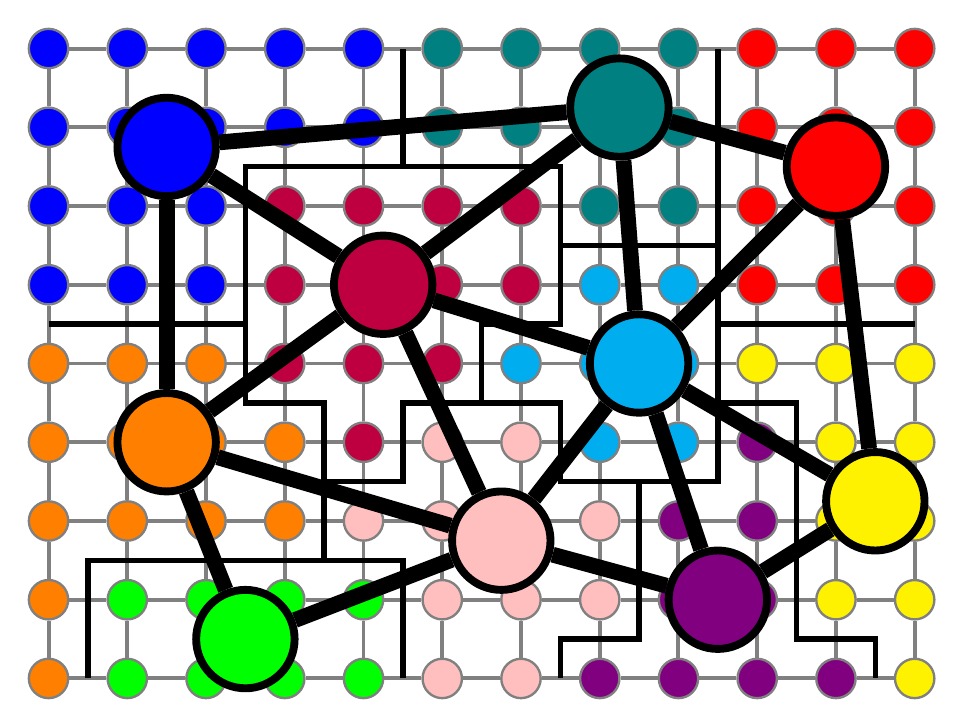
\begin{tikzpicture}
    \node (aa) at  (0,0) [draw,circle,line width=0.3mm,minimum width=0.5cm,draw=gray,fill=orange] {};
    \node (ba) at  (1,0) [draw,circle,line width=0.3mm,minimum width=0.5cm,draw=gray,fill=green] {};
    \node (ca) at  (2,0) [draw,circle,line width=0.3mm,minimum width=0.5cm,draw=gray,fill=green] {};
    \node (da) at  (3,0) [draw,circle,line width=0.3mm,minimum width=0.5cm,draw=gray,fill=green] {};
    \node (ea) at  (4,0) [draw,circle,line width=0.3mm,minimum width=0.5cm,draw=gray,fill=green] {};
    \node (fa) at  (5,0) [draw,circle,line width=0.3mm,minimum width=0.5cm,draw=gray,fill=pink] {};
    \node (ga) at  (6,0) [draw,circle,line width=0.3mm,minimum width=0.5cm,draw=gray,fill=pink] {};
    \node (ha) at  (7,0) [draw,circle,line width=0.3mm,minimum width=0.5cm,draw=gray,fill=violet] {};
    \node (ia) at  (8,0) [draw,circle,line width=0.3mm,minimum width=0.5cm,draw=gray,fill=violet] {};
    \node (ja) at  (9,0) [draw,circle,line width=0.3mm,minimum width=0.5cm,draw=gray,fill=violet] {};
    \node (ka) at (10,0) [draw,circle,line width=0.3mm,minimum width=0.5cm,draw=gray,fill=violet] {};
    \node (la) at (11,0) [draw,circle,line width=0.3mm,minimum width=0.5cm,draw=gray,fill=yellow] {};    

    \node (ab) at  (0,1) [draw,circle,line width=0.3mm,minimum width=0.5cm,draw=gray,fill=orange] {};
    \node (bb) at  (1,1) [draw,circle,line width=0.3mm,minimum width=0.5cm,draw=gray,fill=green] {};
    \node (cb) at  (2,1) [draw,circle,line width=0.3mm,minimum width=0.5cm,draw=gray,fill=green] {};
    \node (db) at  (3,1) [draw,circle,line width=0.3mm,minimum width=0.5cm,draw=gray,fill=green] {};
    \node (eb) at  (4,1) [draw,circle,line width=0.3mm,minimum width=0.5cm,draw=gray,fill=green] {};
    \node (fb) at  (5,1) [draw,circle,line width=0.3mm,minimum width=0.5cm,draw=gray,fill=pink] {};
    \node (gb) at  (6,1) [draw,circle,line width=0.3mm,minimum width=0.5cm,draw=gray,fill=pink] {};
    \node (hb) at  (7,1) [draw,circle,line width=0.3mm,minimum width=0.5cm,draw=gray,fill=pink] {};
    \node (ib) at  (8,1) [draw,circle,line width=0.3mm,minimum width=0.5cm,draw=gray,fill=violet] {};
    \node (jb) at  (9,1) [draw,circle,line width=0.3mm,minimum width=0.5cm,draw=gray,fill=violet] {};
    \node (kb) at (10,1) [draw,circle,line width=0.3mm,minimum width=0.5cm,draw=gray,fill=yellow] {};
    \node (lb) at (11,1) [draw,circle,line width=0.3mm,minimum width=0.5cm,draw=gray,fill=yellow] {};    

    \node (ac) at  (0,2) [draw,circle,line width=0.3mm,minimum width=0.5cm,draw=gray,fill=orange] {};
    \node (bc) at  (1,2) [draw,circle,line width=0.3mm,minimum width=0.5cm,draw=gray,fill=orange] {};
    \node (cc) at  (2,2) [draw,circle,line width=0.3mm,minimum width=0.5cm,draw=gray,fill=orange] {};
    \node (dc) at  (3,2) [draw,circle,line width=0.3mm,minimum width=0.5cm,draw=gray,fill=orange] {};
    \node (ec) at  (4,2) [draw,circle,line width=0.3mm,minimum width=0.5cm,draw=gray,fill=pink] {};
    \node (fc) at  (5,2) [draw,circle,line width=0.3mm,minimum width=0.5cm,draw=gray,fill=pink] {};
    \node (gc) at  (6,2) [draw,circle,line width=0.3mm,minimum width=0.5cm,draw=gray,fill=pink] {};
    \node (hc) at  (7,2) [draw,circle,line width=0.3mm,minimum width=0.5cm,draw=gray,fill=pink] {};
    \node (ic) at  (8,2) [draw,circle,line width=0.3mm,minimum width=0.5cm,draw=gray,fill=violet] {};
    \node (jc) at  (9,2) [draw,circle,line width=0.3mm,minimum width=0.5cm,draw=gray,fill=violet] {};
    \node (kc) at (10,2) [draw,circle,line width=0.3mm,minimum width=0.5cm,draw=gray,fill=yellow] {};
    \node (lc) at (11,2) [draw,circle,line width=0.3mm,minimum width=0.5cm,draw=gray,fill=yellow] {};    

    \node (ad) at  (0,3) [draw,circle,line width=0.3mm,minimum width=0.5cm,draw=gray,fill=orange] {};
    \node (bd) at  (1,3) [draw,circle,line width=0.3mm,minimum width=0.5cm,draw=gray,fill=orange] {};
    \node (cd) at  (2,3) [draw,circle,line width=0.3mm,minimum width=0.5cm,draw=gray,fill=orange] {};
    \node (dd) at  (3,3) [draw,circle,line width=0.3mm,minimum width=0.5cm,draw=gray,fill=orange] {};
    \node (ed) at  (4,3) [draw,circle,line width=0.3mm,minimum width=0.5cm,draw=gray,fill=purple] {};
    \node (fd) at  (5,3) [draw,circle,line width=0.3mm,minimum width=0.5cm,draw=gray,fill=pink] {};
    \node (gd) at  (6,3) [draw,circle,line width=0.3mm,minimum width=0.5cm,draw=gray,fill=pink] {};
    \node (hd) at  (7,3) [draw,circle,line width=0.3mm,minimum width=0.5cm,draw=gray,fill=cyan] {};
    \node (id) at  (8,3) [draw,circle,line width=0.3mm,minimum width=0.5cm,draw=gray,fill=cyan] {};
    \node (jd) at  (9,3) [draw,circle,line width=0.3mm,minimum width=0.5cm,draw=gray,fill=violet] {};
    \node (kd) at (10,3) [draw,circle,line width=0.3mm,minimum width=0.5cm,draw=gray,fill=yellow] {};
    \node (ld) at (11,3) [draw,circle,line width=0.3mm,minimum width=0.5cm,draw=gray,fill=yellow] {};    

    \node (ae) at  (0,4) [draw,circle,line width=0.3mm,minimum width=0.5cm,draw=gray,fill=orange] {};
    \node (be) at  (1,4) [draw,circle,line width=0.3mm,minimum width=0.5cm,draw=gray,fill=orange] {};
    \node (ce) at  (2,4) [draw,circle,line width=0.3mm,minimum width=0.5cm,draw=gray,fill=orange] {};
    \node (de) at  (3,4) [draw,circle,line width=0.3mm,minimum width=0.5cm,draw=gray,fill=purple] {};
    \node (ee) at  (4,4) [draw,circle,line width=0.3mm,minimum width=0.5cm,draw=gray,fill=purple] {};
    \node (fe) at  (5,4) [draw,circle,line width=0.3mm,minimum width=0.5cm,draw=gray,fill=purple] {};
    \node (ge) at  (6,4) [draw,circle,line width=0.3mm,minimum width=0.5cm,draw=gray,fill=cyan] {};
    \node (he) at  (7,4) [draw,circle,line width=0.3mm,minimum width=0.5cm,draw=gray,fill=cyan] {};
    \node (ie) at  (8,4) [draw,circle,line width=0.3mm,minimum width=0.5cm,draw=gray,fill=cyan] {};
    \node (je) at  (9,4) [draw,circle,line width=0.3mm,minimum width=0.5cm,draw=gray,fill=yellow] {};
    \node (ke) at (10,4) [draw,circle,line width=0.3mm,minimum width=0.5cm,draw=gray,fill=yellow] {};
    \node (le) at (11,4) [draw,circle,line width=0.3mm,minimum width=0.5cm,draw=gray,fill=yellow] {};    

    \node (af) at  (0,5) [draw,circle,line width=0.3mm,minimum width=0.5cm,draw=gray,fill=blue] {};
    \node (bf) at  (1,5) [draw,circle,line width=0.3mm,minimum width=0.5cm,draw=gray,fill=blue] {};
    \node (cf) at  (2,5) [draw,circle,line width=0.3mm,minimum width=0.5cm,draw=gray,fill=blue] {};
    \node (df) at  (3,5) [draw,circle,line width=0.3mm,minimum width=0.5cm,draw=gray,fill=purple] {};
    \node (ef) at  (4,5) [draw,circle,line width=0.3mm,minimum width=0.5cm,draw=gray,fill=purple] {};
    \node (ff) at  (5,5) [draw,circle,line width=0.3mm,minimum width=0.5cm,draw=gray,fill=purple] {};
    \node (gf) at  (6,5) [draw,circle,line width=0.3mm,minimum width=0.5cm,draw=gray,fill=purple] {};
    \node (hf) at  (7,5) [draw,circle,line width=0.3mm,minimum width=0.5cm,draw=gray,fill=cyan] {};
    \node (if) at  (8,5) [draw,circle,line width=0.3mm,minimum width=0.5cm,draw=gray,fill=cyan] {};
    \node (jf) at  (9,5) [draw,circle,line width=0.3mm,minimum width=0.5cm,draw=gray,fill=red] {};
    \node (kf) at (10,5) [draw,circle,line width=0.3mm,minimum width=0.5cm,draw=gray,fill=red] {};
    \node (lf) at (11,5) [draw,circle,line width=0.3mm,minimum width=0.5cm,draw=gray,fill=red] {};    
    
    \node (ag) at  (0,6) [draw,circle,line width=0.3mm,minimum width=0.5cm,draw=gray,fill=blue] {};
    \node (bg) at  (1,6) [draw,circle,line width=0.3mm,minimum width=0.5cm,draw=gray,fill=blue] {};
    \node (cg) at  (2,6) [draw,circle,line width=0.3mm,minimum width=0.5cm,draw=gray,fill=blue] {};
    \node (dg) at  (3,6) [draw,circle,line width=0.3mm,minimum width=0.5cm,draw=gray,fill=purple] {};
    \node (eg) at  (4,6) [draw,circle,line width=0.3mm,minimum width=0.5cm,draw=gray,fill=purple] {};
    \node (fg) at  (5,6) [draw,circle,line width=0.3mm,minimum width=0.5cm,draw=gray,fill=purple] {};
    \node (gg) at  (6,6) [draw,circle,line width=0.3mm,minimum width=0.5cm,draw=gray,fill=purple] {};
    \node (hg) at  (7,6) [draw,circle,line width=0.3mm,minimum width=0.5cm,draw=gray,fill=teal] {};
    \node (ig) at  (8,6) [draw,circle,line width=0.3mm,minimum width=0.5cm,draw=gray,fill=teal] {};
    \node (jg) at  (9,6) [draw,circle,line width=0.3mm,minimum width=0.5cm,draw=gray,fill=red] {};
    \node (kg) at (10,6) [draw,circle,line width=0.3mm,minimum width=0.5cm,draw=gray,fill=red] {};
    \node (lg) at (11,6) [draw,circle,line width=0.3mm,minimum width=0.5cm,draw=gray,fill=red] {};    
    
    \node (ah) at  (0,7) [draw,circle,line width=0.3mm,minimum width=0.5cm,draw=gray,fill=blue] {};
    \node (bh) at  (1,7) [draw,circle,line width=0.3mm,minimum width=0.5cm,draw=gray,fill=blue] {};
    \node (ch) at  (2,7) [draw,circle,line width=0.3mm,minimum width=0.5cm,draw=gray,fill=blue] {};
    \node (dh) at  (3,7) [draw,circle,line width=0.3mm,minimum width=0.5cm,draw=gray,fill=blue] {};
    \node (eh) at  (4,7) [draw,circle,line width=0.3mm,minimum width=0.5cm,draw=gray,fill=blue] {};
    \node (fh) at  (5,7) [draw,circle,line width=0.3mm,minimum width=0.5cm,draw=gray,fill=teal] {};
    \node (gh) at  (6,7) [draw,circle,line width=0.3mm,minimum width=0.5cm,draw=gray,fill=teal] {};
    \node (hh) at  (7,7) [draw,circle,line width=0.3mm,minimum width=0.5cm,draw=gray,fill=teal] {};
    \node (ih) at  (8,7) [draw,circle,line width=0.3mm,minimum width=0.5cm,draw=gray,fill=teal] {};
    \node (jh) at  (9,7) [draw,circle,line width=0.3mm,minimum width=0.5cm,draw=gray,fill=red] {};
    \node (kh) at (10,7) [draw,circle,line width=0.3mm,minimum width=0.5cm,draw=gray,fill=red] {};
    \node (lh) at (11,7) [draw,circle,line width=0.3mm,minimum width=0.5cm,draw=gray,fill=red] {};    
    
    \node (ai) at  (0,8) [draw,circle,line width=0.3mm,minimum width=0.5cm,draw=gray,fill=blue] {};
    \node (bi) at  (1,8) [draw,circle,line width=0.3mm,minimum width=0.5cm,draw=gray,fill=blue] {};
    \node (ci) at  (2,8) [draw,circle,line width=0.3mm,minimum width=0.5cm,draw=gray,fill=blue] {};
    \node (di) at  (3,8) [draw,circle,line width=0.3mm,minimum width=0.5cm,draw=gray,fill=blue] {};
    \node (ei) at  (4,8) [draw,circle,line width=0.3mm,minimum width=0.5cm,draw=gray,fill=blue] {};
    \node (fi) at  (5,8) [draw,circle,line width=0.3mm,minimum width=0.5cm,draw=gray,fill=teal] {};
    \node (gi) at  (6,8) [draw,circle,line width=0.3mm,minimum width=0.5cm,draw=gray,fill=teal] {};
    \node (hi) at  (7,8) [draw,circle,line width=0.3mm,minimum width=0.5cm,draw=gray,fill=teal] {};
    \node (ii) at  (8,8) [draw,circle,line width=0.3mm,minimum width=0.5cm,draw=gray,fill=teal] {};
    \node (ji) at  (9,8) [draw,circle,line width=0.3mm,minimum width=0.5cm,draw=gray,fill=red] {};
    \node (ki) at (10,8) [draw,circle,line width=0.3mm,minimum width=0.5cm,draw=gray,fill=red] {};
    \node (li) at (11,8) [draw,circle,line width=0.3mm,minimum width=0.5cm,draw=gray,fill=red] {};    




    \draw[-,line width=0.5mm,color=gray] (aa) to (ba);
    \draw[-,line width=0.5mm,color=gray] (ba) to (ca);
    \draw[-,line width=0.5mm,color=gray] (ca) to (da);
    \draw[-,line width=0.5mm,color=gray] (da) to (ea);
    \draw[-,line width=0.5mm,color=gray] (ea) to (fa);
    \draw[-,line width=0.5mm,color=gray] (fa) to (ga);
    \draw[-,line width=0.5mm,color=gray] (ga) to (ha);
    \draw[-,line width=0.5mm,color=gray] (ha) to (ia);
    \draw[-,line width=0.5mm,color=gray] (ia) to (ja);
    \draw[-,line width=0.5mm,color=gray] (ja) to (ka);
    \draw[-,line width=0.5mm,color=gray] (ka) to (la);

    \draw[-,line width=0.5mm,color=gray] (ab) to (bb);
    \draw[-,line width=0.5mm,color=gray] (bb) to (cb);
    \draw[-,line width=0.5mm,color=gray] (cb) to (db);
    \draw[-,line width=0.5mm,color=gray] (db) to (eb);
    \draw[-,line width=0.5mm,color=gray] (eb) to (fb);
    \draw[-,line width=0.5mm,color=gray] (fb) to (gb);
    \draw[-,line width=0.5mm,color=gray] (gb) to (hb);
    \draw[-,line width=0.5mm,color=gray] (hb) to (ib);
    \draw[-,line width=0.5mm,color=gray] (ib) to (jb);
    \draw[-,line width=0.5mm,color=gray] (jb) to (kb);
    \draw[-,line width=0.5mm,color=gray] (kb) to (lb);

    \draw[-,line width=0.5mm,color=gray] (ac) to (bc);
    \draw[-,line width=0.5mm,color=gray] (bc) to (cc);
    \draw[-,line width=0.5mm,color=gray] (cc) to (dc);
    \draw[-,line width=0.5mm,color=gray] (dc) to (ec);
    \draw[-,line width=0.5mm,color=gray] (ec) to (fc);
    \draw[-,line width=0.5mm,color=gray] (fc) to (gc);
    \draw[-,line width=0.5mm,color=gray] (gc) to (hc);
    \draw[-,line width=0.5mm,color=gray] (hc) to (ic);
    \draw[-,line width=0.5mm,color=gray] (ic) to (jc);
    \draw[-,line width=0.5mm,color=gray] (jc) to (kc);
    \draw[-,line width=0.5mm,color=gray] (kc) to (lc);

    \draw[-,line width=0.5mm,color=gray] (ad) to (bd);
    \draw[-,line width=0.5mm,color=gray] (bd) to (cd);
    \draw[-,line width=0.5mm,color=gray] (cd) to (dd);
    \draw[-,line width=0.5mm,color=gray] (dd) to (ed);
    \draw[-,line width=0.5mm,color=gray] (ed) to (fd);
    \draw[-,line width=0.5mm,color=gray] (fd) to (gd);
    \draw[-,line width=0.5mm,color=gray] (gd) to (hd);
    \draw[-,line width=0.5mm,color=gray] (hd) to (id);
    \draw[-,line width=0.5mm,color=gray] (id) to (jd);
    \draw[-,line width=0.5mm,color=gray] (jd) to (kd);
    \draw[-,line width=0.5mm,color=gray] (kd) to (ld);

    \draw[-,line width=0.5mm,color=gray] (ae) to (be);
    \draw[-,line width=0.5mm,color=gray] (be) to (ce);
    \draw[-,line width=0.5mm,color=gray] (ce) to (de);
    \draw[-,line width=0.5mm,color=gray] (de) to (ee);
    \draw[-,line width=0.5mm,color=gray] (ee) to (fe);
    \draw[-,line width=0.5mm,color=gray] (fe) to (ge);
    \draw[-,line width=0.5mm,color=gray] (ge) to (he);
    \draw[-,line width=0.5mm,color=gray] (he) to (ie);
    \draw[-,line width=0.5mm,color=gray] (ie) to (je);
    \draw[-,line width=0.5mm,color=gray] (je) to (ke);
    \draw[-,line width=0.5mm,color=gray] (ke) to (le);

    \draw[-,line width=0.5mm,color=gray] (ae) to (be);
    \draw[-,line width=0.5mm,color=gray] (be) to (ce);
    \draw[-,line width=0.5mm,color=gray] (ce) to (de);
    \draw[-,line width=0.5mm,color=gray] (de) to (ee);
    \draw[-,line width=0.5mm,color=gray] (ee) to (fe);
    \draw[-,line width=0.5mm,color=gray] (fe) to (ge);
    \draw[-,line width=0.5mm,color=gray] (ge) to (he);
    \draw[-,line width=0.5mm,color=gray] (he) to (ie);
    \draw[-,line width=0.5mm,color=gray] (ie) to (je);
    \draw[-,line width=0.5mm,color=gray] (je) to (ke);
    \draw[-,line width=0.5mm,color=gray] (ke) to (le);

    \draw[-,line width=0.5mm,color=gray] (af) to (bf);
    \draw[-,line width=0.5mm,color=gray] (bf) to (cf);
    \draw[-,line width=0.5mm,color=gray] (cf) to (df);
    \draw[-,line width=0.5mm,color=gray] (df) to (ef);
    \draw[-,line width=0.5mm,color=gray] (ef) to (ff);
    \draw[-,line width=0.5mm,color=gray] (ff) to (gf);
    \draw[-,line width=0.5mm,color=gray] (gf) to (hf);
    \draw[-,line width=0.5mm,color=gray] (hf) to (if);
    \draw[-,line width=0.5mm,color=gray] (if) to (jf);
    \draw[-,line width=0.5mm,color=gray] (jf) to (kf);
    \draw[-,line width=0.5mm,color=gray] (kf) to (lf);

    \draw[-,line width=0.5mm,color=gray] (ag) to (bg);
    \draw[-,line width=0.5mm,color=gray] (bg) to (cg);
    \draw[-,line width=0.5mm,color=gray] (cg) to (dg);
    \draw[-,line width=0.5mm,color=gray] (dg) to (eg);
    \draw[-,line width=0.5mm,color=gray] (eg) to (fg);
    \draw[-,line width=0.5mm,color=gray] (fg) to (gg);
    \draw[-,line width=0.5mm,color=gray] (gg) to (hg);
    \draw[-,line width=0.5mm,color=gray] (hg) to (ig);
    \draw[-,line width=0.5mm,color=gray] (ig) to (jg);
    \draw[-,line width=0.5mm,color=gray] (jg) to (kg);
    \draw[-,line width=0.5mm,color=gray] (kg) to (lg);

    \draw[-,line width=0.5mm,color=gray] (ah) to (bh);
    \draw[-,line width=0.5mm,color=gray] (bh) to (ch);
    \draw[-,line width=0.5mm,color=gray] (ch) to (dh);
    \draw[-,line width=0.5mm,color=gray] (dh) to (eh);
    \draw[-,line width=0.5mm,color=gray] (eh) to (fh);
    \draw[-,line width=0.5mm,color=gray] (fh) to (gh);
    \draw[-,line width=0.5mm,color=gray] (gh) to (hh);
    \draw[-,line width=0.5mm,color=gray] (hh) to (ih);
    \draw[-,line width=0.5mm,color=gray] (ih) to (jh);
    \draw[-,line width=0.5mm,color=gray] (jh) to (kh);
    \draw[-,line width=0.5mm,color=gray] (kh) to (lh);

    \draw[-,line width=0.5mm,color=gray] (ai) to (bi);
    \draw[-,line width=0.5mm,color=gray] (bi) to (ci);
    \draw[-,line width=0.5mm,color=gray] (ci) to (di);
    \draw[-,line width=0.5mm,color=gray] (di) to (ei);
    \draw[-,line width=0.5mm,color=gray] (ei) to (fi);
    \draw[-,line width=0.5mm,color=gray] (fi) to (gi);
    \draw[-,line width=0.5mm,color=gray] (gi) to (hi);
    \draw[-,line width=0.5mm,color=gray] (hi) to (ii);
    \draw[-,line width=0.5mm,color=gray] (ii) to (ji);
    \draw[-,line width=0.5mm,color=gray] (ji) to (ki);
    \draw[-,line width=0.5mm,color=gray] (ki) to (li);




    \draw[-,line width=0.5mm,color=gray] (aa) to (ab);
    \draw[-,line width=0.5mm,color=gray] (ab) to (ac);
    \draw[-,line width=0.5mm,color=gray] (ac) to (ad);
    \draw[-,line width=0.5mm,color=gray] (ad) to (ae);
    \draw[-,line width=0.5mm,color=gray] (ae) to (af);
    \draw[-,line width=0.5mm,color=gray] (af) to (ag);
    \draw[-,line width=0.5mm,color=gray] (ag) to (ah);
    \draw[-,line width=0.5mm,color=gray] (ah) to (ai);

    \draw[-,line width=0.5mm,color=gray] (ba) to (bb);
    \draw[-,line width=0.5mm,color=gray] (bb) to (bc);
    \draw[-,line width=0.5mm,color=gray] (bc) to (bd);
    \draw[-,line width=0.5mm,color=gray] (bd) to (be);
    \draw[-,line width=0.5mm,color=gray] (be) to (bf);
    \draw[-,line width=0.5mm,color=gray] (bf) to (bg);
    \draw[-,line width=0.5mm,color=gray] (bg) to (bh);
    \draw[-,line width=0.5mm,color=gray] (bh) to (bi);

    \draw[-,line width=0.5mm,color=gray] (ca) to (cb);
    \draw[-,line width=0.5mm,color=gray] (cb) to (cc);
    \draw[-,line width=0.5mm,color=gray] (cc) to (cd);
    \draw[-,line width=0.5mm,color=gray] (cd) to (ce);
    \draw[-,line width=0.5mm,color=gray] (ce) to (cf);
    \draw[-,line width=0.5mm,color=gray] (cf) to (cg);
    \draw[-,line width=0.5mm,color=gray] (cg) to (ch);
    \draw[-,line width=0.5mm,color=gray] (ch) to (ci);
    
    \draw[-,line width=0.5mm,color=gray] (da) to (db);
    \draw[-,line width=0.5mm,color=gray] (db) to (dc);
    \draw[-,line width=0.5mm,color=gray] (dc) to (dd);
    \draw[-,line width=0.5mm,color=gray] (dd) to (de);
    \draw[-,line width=0.5mm,color=gray] (de) to (df);
    \draw[-,line width=0.5mm,color=gray] (df) to (dg);
    \draw[-,line width=0.5mm,color=gray] (dg) to (dh);
    \draw[-,line width=0.5mm,color=gray] (dh) to (di);
    
    \draw[-,line width=0.5mm,color=gray] (ea) to (eb);
    \draw[-,line width=0.5mm,color=gray] (eb) to (ec);
    \draw[-,line width=0.5mm,color=gray] (ec) to (ed);
    \draw[-,line width=0.5mm,color=gray] (ed) to (ee);
    \draw[-,line width=0.5mm,color=gray] (ee) to (ef);
    \draw[-,line width=0.5mm,color=gray] (ef) to (eg);
    \draw[-,line width=0.5mm,color=gray] (eg) to (eh);
    \draw[-,line width=0.5mm,color=gray] (eh) to (ei);
    
    \draw[-,line width=0.5mm,color=gray] (fa) to (fb);
    \draw[-,line width=0.5mm,color=gray] (fb) to (fc);
    \draw[-,line width=0.5mm,color=gray] (fc) to (fd);
    \draw[-,line width=0.5mm,color=gray] (fd) to (fe);
    \draw[-,line width=0.5mm,color=gray] (fe) to (ff);
    \draw[-,line width=0.5mm,color=gray] (ff) to (fg);
    \draw[-,line width=0.5mm,color=gray] (fg) to (fh);
    \draw[-,line width=0.5mm,color=gray] (fh) to (fi);

    \draw[-,line width=0.5mm,color=gray] (ga) to (gb);
    \draw[-,line width=0.5mm,color=gray] (gb) to (gc);
    \draw[-,line width=0.5mm,color=gray] (gc) to (gd);
    \draw[-,line width=0.5mm,color=gray] (gd) to (ge);
    \draw[-,line width=0.5mm,color=gray] (ge) to (gf);
    \draw[-,line width=0.5mm,color=gray] (gf) to (gg);
    \draw[-,line width=0.5mm,color=gray] (gg) to (gh);
    \draw[-,line width=0.5mm,color=gray] (gh) to (gi);

    \draw[-,line width=0.5mm,color=gray] (ha) to (hb);
    \draw[-,line width=0.5mm,color=gray] (hb) to (hc);
    \draw[-,line width=0.5mm,color=gray] (hc) to (hd);
    \draw[-,line width=0.5mm,color=gray] (hd) to (he);
    \draw[-,line width=0.5mm,color=gray] (he) to (hf);
    \draw[-,line width=0.5mm,color=gray] (hf) to (hg);
    \draw[-,line width=0.5mm,color=gray] (hg) to (hh);
    \draw[-,line width=0.5mm,color=gray] (hh) to (hi);

    \draw[-,line width=0.5mm,color=gray] (ia) to (ib);
    \draw[-,line width=0.5mm,color=gray] (ib) to (ic);
    \draw[-,line width=0.5mm,color=gray] (ic) to (id);
    \draw[-,line width=0.5mm,color=gray] (id) to (ie);
    \draw[-,line width=0.5mm,color=gray] (ie) to (if);
    \draw[-,line width=0.5mm,color=gray] (if) to (ig);
    \draw[-,line width=0.5mm,color=gray] (ig) to (ih);
    \draw[-,line width=0.5mm,color=gray] (ih) to (ii);

    \draw[-,line width=0.5mm,color=gray] (ja) to (jb);
    \draw[-,line width=0.5mm,color=gray] (jb) to (jc);
    \draw[-,line width=0.5mm,color=gray] (jc) to (jd);
    \draw[-,line width=0.5mm,color=gray] (jd) to (je);
    \draw[-,line width=0.5mm,color=gray] (je) to (jf);
    \draw[-,line width=0.5mm,color=gray] (jf) to (jg);
    \draw[-,line width=0.5mm,color=gray] (jg) to (jh);
    \draw[-,line width=0.5mm,color=gray] (jh) to (ji);

    \draw[-,line width=0.5mm,color=gray] (ka) to (kb);
    \draw[-,line width=0.5mm,color=gray] (kb) to (kc);
    \draw[-,line width=0.5mm,color=gray] (kc) to (kd);
    \draw[-,line width=0.5mm,color=gray] (kd) to (ke);
    \draw[-,line width=0.5mm,color=gray] (ke) to (kf);
    \draw[-,line width=0.5mm,color=gray] (kf) to (kg);
    \draw[-,line width=0.5mm,color=gray] (kg) to (kh);
    \draw[-,line width=0.5mm,color=gray] (kh) to (ki);

    \draw[-,line width=0.5mm,color=gray] (la) to (lb);
    \draw[-,line width=0.5mm,color=gray] (lb) to (lc);
    \draw[-,line width=0.5mm,color=gray] (lc) to (ld);
    \draw[-,line width=0.5mm,color=gray] (ld) to (le);
    \draw[-,line width=0.5mm,color=gray] (le) to (lf);
    \draw[-,line width=0.5mm,color=gray] (lf) to (lg);
    \draw[-,line width=0.5mm,color=gray] (lg) to (lh);
    \draw[-,line width=0.5mm,color=gray] (lh) to (li);




    \draw[-,line width=0.7mm] (0.5,0) to (0.5,1.5);
    \draw[-,line width=0.7mm] (0.465,1.5) to (4.535,1.5);
    \draw[-,line width=0.7mm] (4.5,0) to (4.5,1.5);
    \draw[-,line width=0.7mm] (3.5,1.5) to (3.5,3.535);
    \draw[-,line width=0.7mm] (3.5,3.5) to (2.465,3.5);
    \draw[-,line width=0.7mm] (2.5,3.5) to (2.5,6.5);
    \draw[-,line width=0.7mm] (0,4.5) to (2.5,4.5);
    \draw[-,line width=0.7mm] (2.465,6.5) to (6.535,6.5);
    \draw[-,line width=0.7mm] (4.5,6.5) to (4.5,8);
    \draw[-,line width=0.7mm] (6.5,6.5) to (6.5,4.465);
    \draw[-,line width=0.7mm] (6.5,4.5) to (5.465,4.5);
    \draw[-,line width=0.7mm] (5.5,4.5) to (5.5,3.5);
    \draw[-,line width=0.7mm] (4.5,3.5) to (6.535,3.5);
    \draw[-,line width=0.7mm] (4.5,3.535) to (4.5,2.465);
    \draw[-,line width=0.7mm] (3.5,2.5) to (4.5,2.5);
    \draw[-,line width=0.7mm] (6.5,5.5) to (8.5,5.5);
    \draw[-,line width=0.7mm] (8.5,2.465) to (8.5,8);
    \draw[-,line width=0.7mm] (6.5,3.5) to (6.5,2.465);
    \draw[-,line width=0.7mm] (6.5,2.5) to (8.5,2.5);
    \draw[-,line width=0.7mm] (7.5,2.5) to (7.5,0.465);
    \draw[-,line width=0.7mm] (8.5,4.5) to (11,4.5);
    \draw[-,line width=0.7mm] (8.5,3.5) to (9.5,3.5);
    \draw[-,line width=0.7mm] (6.5,0) to (6.5,0.535);
    \draw[-,line width=0.7mm] (6.5,0.5) to (7.5,0.5);
    \draw[-,line width=0.7mm] (9.5,0.5) to (9.5,3.535);
    \draw[-,line width=0.7mm] (9.465,0.5) to (10.535,0.5);
    \draw[-,line width=0.7mm] (10.5,0.5) to (10.5,0);




    \node (orange) at (1.5,3) [draw,circle,line width=1mm,minimum width=1.25cm,fill=orange] {};    
    \node (green) at (2.5,0.5) [draw,circle,line width=1mm,minimum width=1.25cm,fill=green] {};    
    \node (blue) at (1.5,6.75) [draw,circle,line width=1mm,minimum width=1.25cm,fill=blue] {};    
    \node (purple) at (4.25,5) [draw,circle,line width=1mm,minimum width=1.25cm,fill=purple] {};    
    \node (pink) at (5.75,1.75) [draw,circle,line width=1mm,minimum width=1.25cm,fill=pink] {};    
    \node (cyan) at (7.5,4) [draw,circle,line width=1mm,minimum width=1.25cm,fill=cyan] {};    
    \node (teal) at (7.25,7.25) [draw,circle,line width=1mm,minimum width=1.25cm,fill=teal] {};    
    \node (violet) at (8.5,1) [draw,circle,line width=1mm,minimum width=1.25cm,fill=violet] {};    
    \node (yellow) at (10.5,2.25) [draw,circle,line width=1mm,minimum width=1.25cm,fill=yellow] {};    
    \node (red) at (10,6.5) [draw,circle,line width=1mm,minimum width=1.25cm,fill=red] {};    



    \draw[-,line width=2mm] (blue) to (orange);
    \draw[-,line width=2mm] (blue) to (purple);
    \draw[-,line width=2mm] (blue) to (teal);
    \draw[-,line width=2mm] (orange) to (purple);
    \draw[-,line width=2mm] (orange) to (green);
    \draw[-,line width=2mm] (orange) to (pink);
    \draw[-,line width=2mm] (green) to (pink);
    \draw[-,line width=2mm] (purple) to (teal);
    \draw[-,line width=2mm] (purple) to (cyan);
    \draw[-,line width=2mm] (purple) to (pink);
    \draw[-,line width=2mm] (teal) to (red);
    \draw[-,line width=2mm] (teal) to (cyan);
    \draw[-,line width=2mm] (cyan) to (pink);
    \draw[-,line width=2mm] (cyan) to (violet);
    \draw[-,line width=2mm] (cyan) to (yellow);
    \draw[-,line width=2mm] (cyan) to (red);
    \draw[-,line width=2mm] (pink) to (violet);
    \draw[-,line width=2mm] (yellow) to (red);
    \draw[-,line width=2mm] (yellow) to (violet);

\end{tikzpicture}
}
        \caption{The corresponding region adjacency graph.}
    \end{subfigure}
    \caption[Pixel to Region Conversion]{Converting a pixel adjacency graph to a region adjacency graph.}
    \label{fig:pixelToRegion}
\end{figure}
\smallskip \\ \indent
To achieve this, the notion of similarity of pixels must be quantified. An unsophisticated method might convert the pixel adjacency graph into a weighted graph, creating a formula converting the difference in the intensity of the pixels to a weight. An example of this is normalising the difference between values - if the pixels have precisely the same intensity, give their edge a weight of $1$; if they are exact opposites (i.e., one black and one white), give their edge a weight of $0$. Once this has been completed, nodes with sufficiently high weight can be combined into a single node. 
\smallskip \\ \indent
Immediate issues begin to arise when considering this method. Firstly, what function should be used to assign weights? Secondly, how should nodes be combined if the pixels have different values? Should the mean value be taken? The median? One chosen at random? Moreover, how many nodes should be combined? What will happen if too many or too few are collected together?
\smallskip \\ \indent
The concerns surrounding weighting edges indicate that this problem may be more complicated than it first appears. In fact, grouping the nodes is a form of low-level image segmentation. While this makes the problem more computationally complex, it has the advantage that there exist well-established algorithms providing reasonable solutions to it. Unsupervised clustering algorithms such as \textit{the watershed transform} \cite{Watershed} or \textit{k-means clustering} \cite{KMeans} are two such methods that have been applied to this problem previously.
\smallskip \\ \indent
More importantly to this investigation, the number of regions in the image will directly impact the transmission time. Reducing the number of nodes in the graph is advantageous because it reduces the amount of data transmitted. However, in doing so, it also reduces the image's resolution. Consequently, removing too many nodes from the graph will remove any clarity of the contents of the image, making the process worthless. Figure \ref{fig:regions} depicts this. Therefore, this balance must be struck heuristically to find the optimal point between maximising performance benefits and minimising loss of image data. Moreover, this optimal point is likely to be different for every image, adding a further layer of complexity.
\begin{figure}[htp]
    \centering
    \begin{subfigure}[t]{0.29\textwidth}
        \centering
        \captionsetup{justification=centering}
        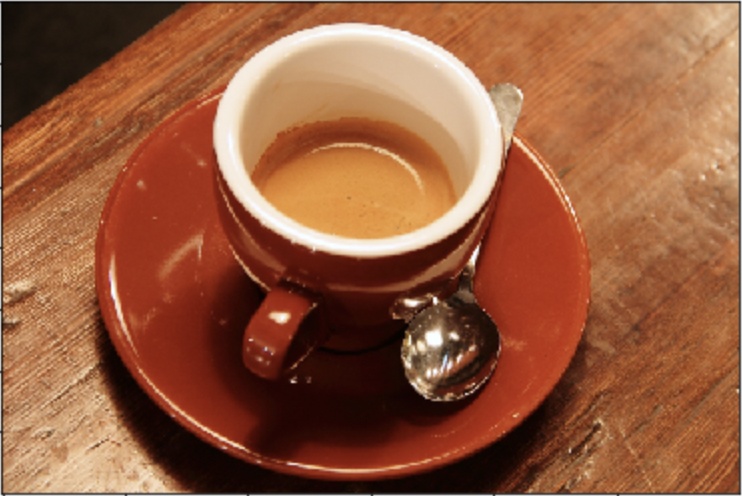
\includegraphics[scale=0.34]{figures/adjacencyBefore}
        \caption{A photograph of a cup of coffee.}
    \end{subfigure} \hfill%
    \begin{subfigure}[t]{0.29\textwidth}
        \centering
        \captionsetup{justification=centering}
        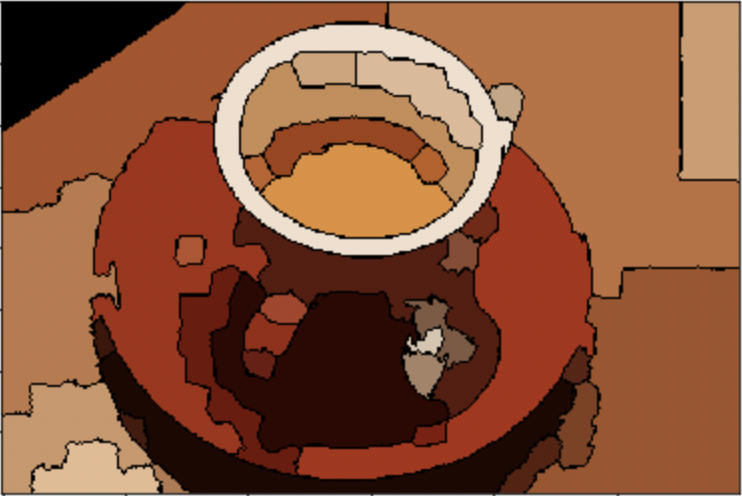
\includegraphics[scale=0.34]{figures/adjacencyMiddle}
        \caption{The picture of coffee split into approximately 400 regions.}
    \end{subfigure} \hfill%
    \begin{subfigure}[t]{0.29\textwidth}
        \centering
        \captionsetup{justification=centering}
        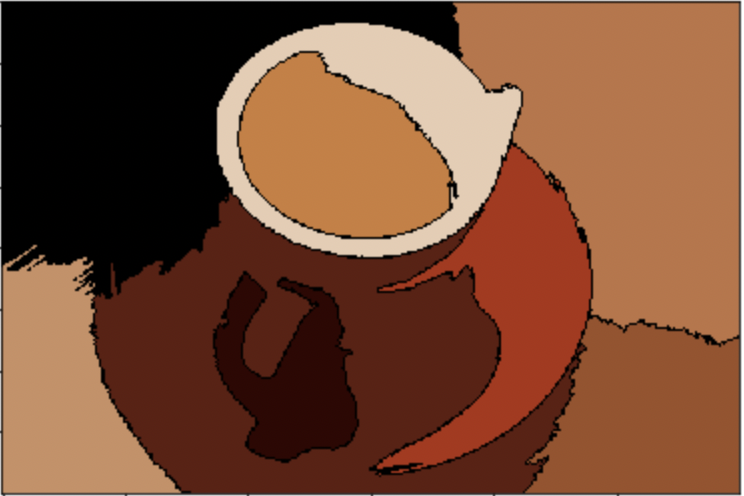
\includegraphics[scale=0.34]{figures/adjacencyAfter}
        \caption{The picture of coffee split into approximately 10 regions.}
    \end{subfigure}%
    \caption[Tuning Region Adjacency Graphs]{A demonstration of the impact of reducing the number of regions on image quality. Images taken from \cite{Foveal}.}
    \label{fig:regions}
\end{figure}
\smallskip \\ \indent
Using similar techniques to seam carving, it is possible to make this trade-off less severe. For example, \textit{Foveal sampling} is a method of recreating the visual activity of the eye in the mapping of an image ~\cite{Foveal}. The \textit{Fovea centralis} is a region of the retina responsible for the sharp central vision used by mammals to focus on particular objects. Foveal sampling uses the shape of the Fovea centralis to produce a graph that can be overlayed onto an image, extracting the areas that an observer will focus on. Consequently, more regions are created in areas critical to perception, and fewer in areas out of focus. This allows the region budget to be more efficiently used, so the overall number required can be smaller without impacting image quality as significantly. Similar techniques have been applied using saliency maps or other methods for determining the importance of regions in an image.
\begin{figure}[htp]
    \centering
    \begin{subfigure}[t]{0.29\textwidth}
        \centering
        \captionsetup{justification=centering}
        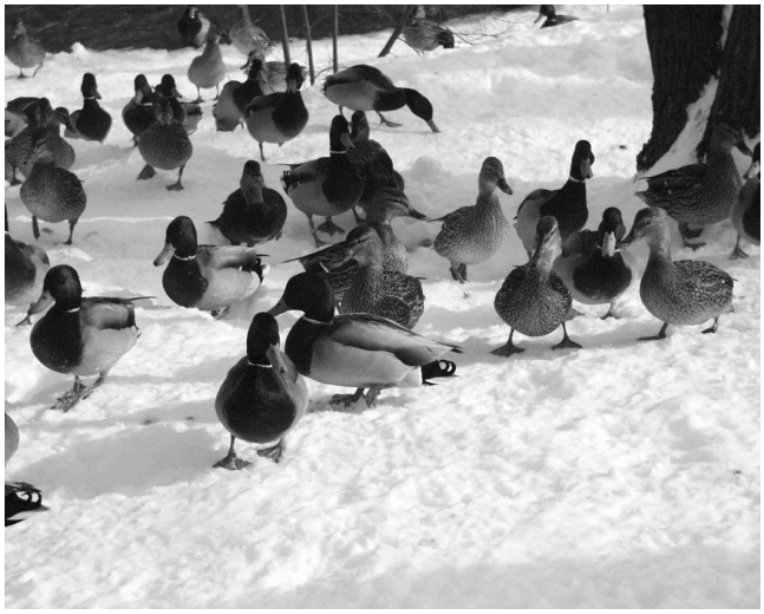
\includegraphics[scale=0.34]{figures/fovealBefore}
        \caption{A photograph of some ducks.}
    \end{subfigure} \hfill%
    \begin{subfigure}[t]{0.29\textwidth}
        \centering
        \captionsetup{justification=centering}
        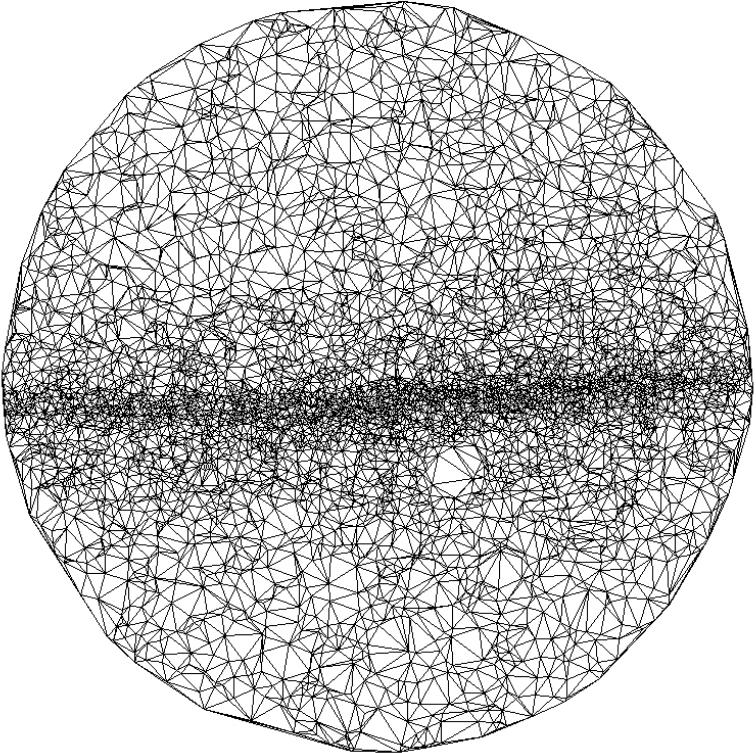
\includegraphics[scale=0.34]{figures/fovealMap}
        \caption{The retinal topography of a kangaroo.}
    \end{subfigure} \hfill%
    \begin{subfigure}[t]{0.29\textwidth}
        \centering
        \captionsetup{justification=centering}
        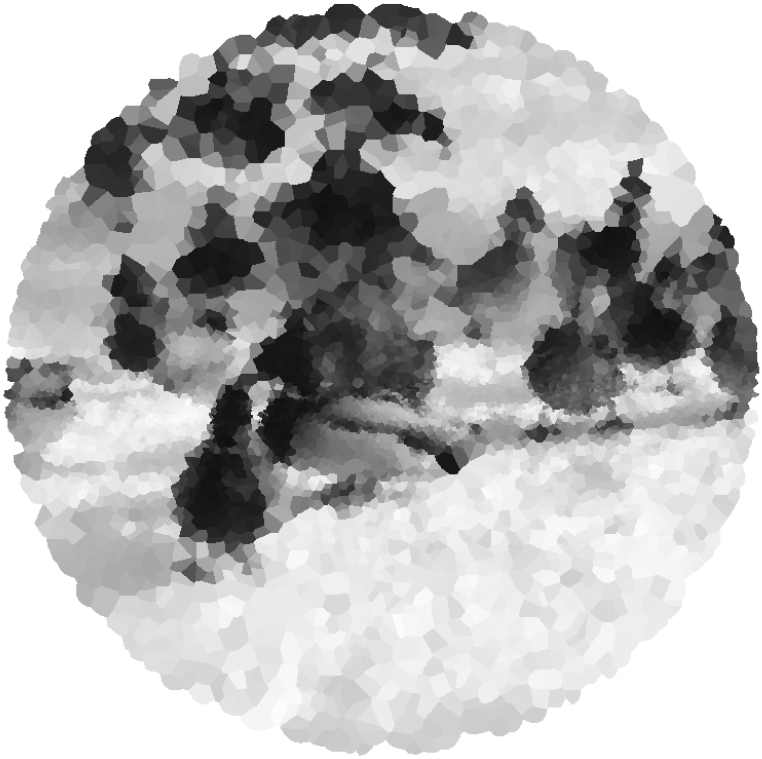
\includegraphics[scale=0.34]{figures/fovealResult}
        \caption{The photograph of ducks sampled using the retinal topography of a kangaroo.}
    \end{subfigure}%
    \caption[Foveal Sampling]{An example of foveal sampling. Images taken from \cite{Foveal}.}
    \label{fig:foveal}
\end{figure}

\setlength{\leftskip}{0cm}
\subsection{Transmission Rate}
\label{sec:parallelisation}
\setlength{\leftskip}{0.5cm}
\indent \indent
Where the previous sections aimed to improve video transmission time by reducing the size of video files, this section targets the bottlenecks limiting the transmission rate of the system. To do this, the project investigates the application of parallel computing.
\smallskip \\ \indent
Parallel computing is often conflated with \textit{concurrent computing}. However, the terms are distinct, and can exist both separately and together. In parallel computing, a task is broken down into numerous, very similar sub-tasks that can be completed independently and recombined later ~\cite{ParallelismVsConcurrency}. In concurrent computing, the various sub-tasks will address unrelated processes varying in nature, often requiring inter-process communication during execution ~\cite{ParallelismVsConcurrency}. This area of the project began considering parallelisation alone to attempt to maximise performance gains, but expanded into concurrency as the breadth of functionality that could benefit from these modifications became apparent. In Figure \ref{fig:parallelStack}, the abstract layers of the networking processes have been coloured to indicate whether concurrent or parallel computing is used.
\begin{figure}[htp]
    \centering
    \scalebox{0.6}{\begin{tikzpicture}
    \node (videoa2) at (0.4,0.4) [draw,thick,minimum width=5cm,minimum height=5cm,fill=abstractYellow] {};
    \node (videoa1) at (0.2,0.2) [draw,thick,minimum width=5cm,minimum height=5cm,fill=abstractYellow] {};
    \node (videoa0) at (0,0) [draw,thick,minimum width=5cm,minimum height=5cm,fill=abstractYellow] {\LARGE\textrm{Video}};


    \node (packing) at (7,0) [draw,thick,minimum width=5cm,minimum height=2cm,fill=mekksBlue] {\LARGE\textrm{Packing}};


    \node (packeta1)  at (13.6,2.175) [draw,thick,minimum width=5cm,minimum height=0.35cm,fill=abstractYellow] {};
    \node (packeta2)  at (13.6,1.7) [draw,thick,minimum width=5cm,minimum height=0.35cm,fill=abstractYellow] {};
    \node (packeta3)  at (13.6,1.225) [draw,thick,minimum width=5cm,minimum height=0.35cm,fill=abstractYellow] {};
    \node (packeta4)  at (13.6,0.75) [draw,thick,minimum width=5cm,minimum height=0.35cm,fill=abstractYellow] {};
    \node (packeta5)  at (13.6,0.275) [draw,thick,minimum width=5cm,minimum height=0.35cm,fill=abstractYellow] {};
    \node (packeta6)  at (13.6,-0.2) [draw,thick,minimum width=5cm,minimum height=0.35cm,fill=abstractYellow] {};
    \node (packeta7)  at (13.6,-0.675) [draw,thick,minimum width=5cm,minimum height=0.35cm,fill=abstractYellow] {};
    \node (packeta8)  at (13.6,-1.15) [draw,thick,minimum width=5cm,minimum height=0.35cm,fill=abstractYellow] {};
    \node (packeta9)  at (13.6,-1.625) [draw,thick,minimum width=5cm,minimum height=0.35cm,fill=abstractYellow] {};
    \node (packeta10) at (13.6,-2.1) [draw,thick,minimum width=5cm,minimum height=0.35cm,fill=abstractYellow] {};


    \node (send) at (20.2,0) [draw,thick,minimum width=5cm,minimum height=2cm,fill=ckksRed] {\LARGE\textrm{Send}};


    \node (receive) at (20.2,-7) [draw,thick,minimum width=5cm,minimum height=2cm,fill=ckksRed] {\LARGE\textrm{Receive}};


    \node (packetb1)  at (13.6,-4.825) [draw,thick,minimum width=5cm,minimum height=0.35cm,fill=abstractYellow] {};
    \node (packetb2)  at (13.6,-5.3) [draw,thick,minimum width=5cm,minimum height=0.35cm,fill=abstractYellow] {};
    \node (packetb3)  at (13.6,-5.775) [draw,thick,minimum width=5cm,minimum height=0.35cm,fill=abstractYellow] {};
    \node (packetb4)  at (13.6,-6.25) [draw,thick,minimum width=5cm,minimum height=0.35cm,fill=abstractYellow] {};
    \node (packetb5)  at (13.6,-6.725) [draw,thick,minimum width=5cm,minimum height=0.35cm,fill=abstractYellow] {};
    \node (packetb6)  at (13.6,-7.2) [draw,thick,minimum width=5cm,minimum height=0.35cm,fill=abstractYellow] {};
    \node (packetb7)  at (13.6,-7.675) [draw,thick,minimum width=5cm,minimum height=0.35cm,fill=abstractYellow] {};
    \node (packetb8)  at (13.6,-8.15) [draw,thick,minimum width=5cm,minimum height=0.35cm,fill=abstractYellow] {};
    \node (packetb9)  at (13.6,-8.625) [draw,thick,minimum width=5cm,minimum height=0.35cm,fill=abstractYellow] {};
    \node (packetb10) at (13.6,-9.1) [draw,thick,minimum width=5cm,minimum height=0.35cm,fill=abstractYellow] {};


    \node (unpacking) at (7,-7) [draw,thick,minimum width=5cm,minimum height=2cm,fill=mekksBlue] {\LARGE\textrm{Unpacking}};


    \node (videob2) at (0.4,-6.6) [draw,thick,minimum width=5cm,minimum height=5cm,fill=abstractYellow] {};
    \node (videob1) at (0.2,-6.8) [draw,thick,minimum width=5cm,minimum height=5cm,fill=abstractYellow] {};
    \node (videob0) at (0,-7) [draw,thick,minimum width=5cm,minimum height=5cm,fill=abstractYellow] {\LARGE\textrm{Video}};


    \draw[->,>=stealth,line width=1mm] ([xshift=0.4cm]videoa0.east) to (packing.west);
    \draw[->,>=stealth,line width=1mm] (packing.east) to ([yshift=-0.25cm]packeta5.west);
    \draw[->,>=stealth,line width=1mm] ([yshift=-0.25cm]packeta5.east) to (send.west);

    \draw[->,>=stealth,line width=1mm] ([xshift=-2cm]send.south) to ([xshift=-2cm]receive.north);
    \draw[->,>=stealth,line width=1mm] ([xshift=-1.5cm]send.south) to ([xshift=-1.5cm]receive.north);
    \draw[->,>=stealth,line width=1mm] ([xshift=-1cm]send.south) to ([xshift=-1cm]receive.north);
    \draw[->,>=stealth,line width=1mm] ([xshift=-0.5cm]send.south) to ([xshift=-0.5cm]receive.north);
    \draw[->,>=stealth,line width=1mm] ([xshift=0cm]send.south) to ([xshift=0cm]receive.north);
    \draw[->,>=stealth,line width=1mm] ([xshift=0.5cm]send.south) to ([xshift=0.5cm]receive.north);
    \draw[->,>=stealth,line width=1mm] ([xshift=1cm]send.south) to ([xshift=1cm]receive.north);
    \draw[->,>=stealth,line width=1mm] ([xshift=1.5cm]send.south) to ([xshift=1.5cm]receive.north);
    \draw[->,>=stealth,line width=1mm] ([xshift=2cm]send.south) to ([xshift=2cm]receive.north);

    \draw[->,>=stealth,line width=1mm] (receive.west) to ([yshift=-0.25cm]packetb5.east);
    \draw[->,>=stealth,line width=1mm] ([yshift=-0.25cm]packetb5.west) to (unpacking.east);
    \draw[->,>=stealth,line width=1mm] (unpacking.west) to ([xshift=0.4cm]videob0.east);
\end{tikzpicture}
}
    \captionsetup{justification=centering}
    \caption[Abstract view of parallel processes]{The stages required for a video to be sent across the network.\medskip\\Parallel processes:\sethlcolor{ckksRed} \hl{\quad\quad\quad\quad}\smallskip\\Concurrent processes:\sethlcolor{mekksBlue} \hl{\quad\quad\quad\quad}}
    \label{fig:parallelStack}
\end{figure}
\smallskip \\ \indent
Traditionally, computer design has focussed on \textit{serial computation}. To solve a computational problem, a sequence of instructions was written, they were executed in order, and a result was returned. As predicted by Moore's law, technology scaling was able to double the performance of processors so that they could compute more complex expressions more efficiently for decades ~\cite{Moore}. However, factors like Dennard scaling mean this cannot last forever ~\cite{Dennard}. Therefore, to continue improving performance, computer architects turned to multiprocessing. Rather than making processor components more efficient so that a single instruction executes faster, similar performance gains can be made by executing multiple instructions simultaneously. Consequently, since evidence suggests processors will continue to be optimised to parallel computation, this seemed like a viable opportunity for investigating where performance might be gained in future iterations of surveillance technology.

\setlength{\leftskip}{0cm}
\subsubsection{Communication}
\setlength{\leftskip}{0.5cm}
\indent \indent
Parallelisation already exists in some communication protocols. The \textit{transmission control protocol} (TCP) uses a \textit{sliding window protocol} to send a group of data packets concurrently, ensuring they are ordered correctly at the receiving end. Figure \ref{fig:slidingWindow} depicts this. This and similar protocols exist in the \textit{data-link} layer of the \textit{OSI network model}. The goal of this section of the investigation was to attempt to move the parallelisation higher up the abstract stack.
\begin{figure}[htp]
    \begin{subfigure}[b]{0.45\textwidth}
        \centering
        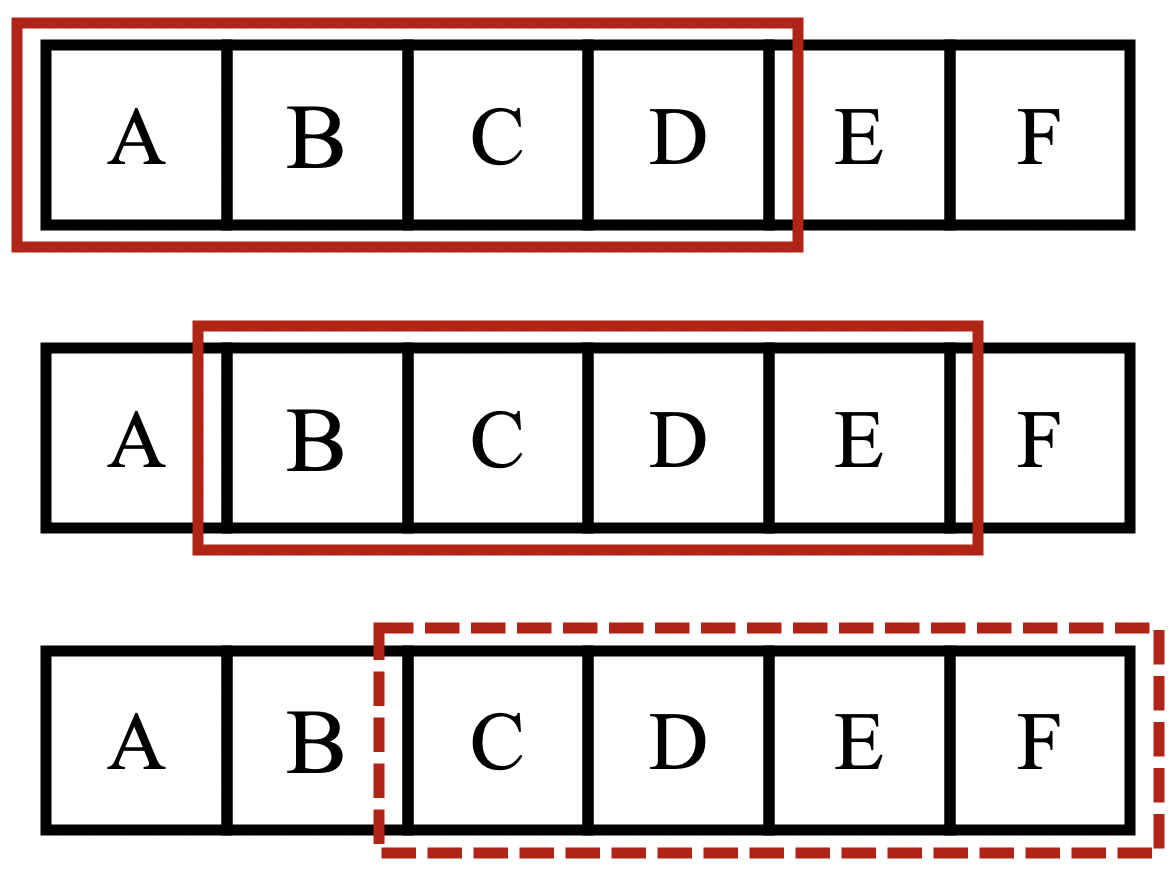
\includegraphics[scale=0.3]{figures/slidingWindow1}
        \caption{The sliding window (red) moves across the packets as each one is sent. Initially the first four packets are sent (top). When packet A is acknowledged, the window slides along one, and E is sent (middle). After the acknowledgement for B is received the window will slide along and F will eventually be sent (bottom).}
    \end{subfigure}\hfill%
    \begin{subfigure}[b]{0.45\textwidth}
        \centering
        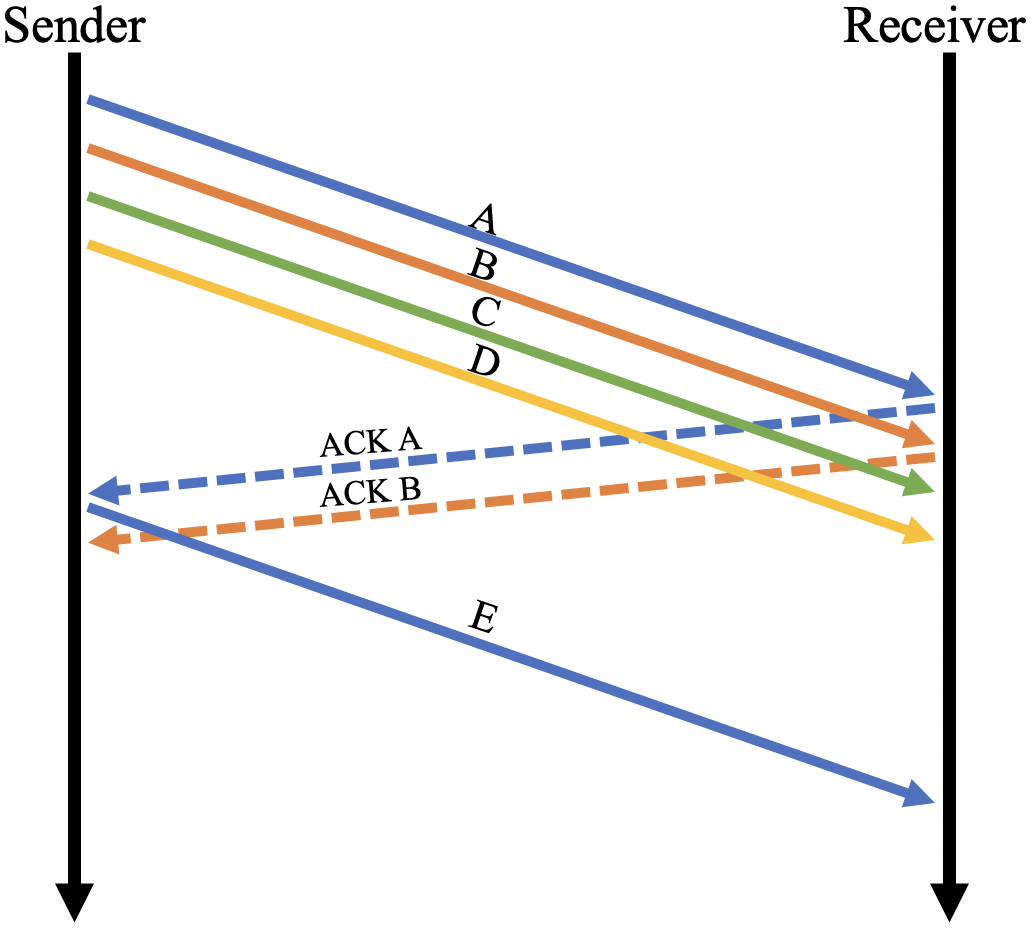
\includegraphics[scale=0.35]{figures/slidingWindow2}
        \caption{The packets currently in the window are sent at the same time, without waiting for any acknowledges. Once an acknowledgment has been received, the next packet in the queue can be sent.}
    \end{subfigure}%
    \caption[The Sliding Window Protocol]{A high-level view of TCP's sliding window protocol.}
    \label{fig:slidingWindow}
\end{figure}
\smallskip \\ \indent
Taking inspiration from sliding windows, instead of sending all video data in a single stream, videos are split into frames, and each frame is divided into packets. Meanwhile, a pool of threads can be created to represent the size of the window. When a packet is ready to be sent, it is assigned a thread from the pool, and the thread establishes a connection with the server, transmitting the data. Consequently, multiple connections will be open in parallel, so, in a given moment, more data will be sent.
\smallskip \\ \indent
However, there are limitations to this technique. Firstly, more data will have to be transmitted than in sequential communication. The algorithm is non-deterministic, so there can be no guarantees about the order in which the packets will arrive after transmission. Consequently, further information must be provided to ensure videos are reassembled correctly. More specifically, a frame number and packet identifier will have to be attached to each packet. While this is worth noting, the size of this additional data is negligible compared to HE data, so it is not a critical issue.
\smallskip \\ \indent
A more pressing concern is the overhead of creating threads and establishing connections. The cost is such that creating too many threads will remove parallelisation benefits or even go so far as to make data transmission slower. Consequently, an optimal balance between the cost of parallelisation and the amount of data to send must be found to maximise gains from this approach.

\setlength{\leftskip}{0cm}
\subsubsection{Data Manipulation}
\setlength{\leftskip}{0.5cm}
\indent \indent
Splitting videos into small packets has further advantages. Before data can be sent from the client to the server, and vice versa, it must be prepared. This can be referred to as \textit{packing} the data. Similarly, when it arrives at its destination, data must be reorganised, or \textit{unpacked}.
\smallskip \\ \indent
Succinctly depicted by Figure \ref{fig:packingAndUnpacking}, there are three distinct stages of the packing in the client \textit{encryption}, \textit{compression}, and \textit{serialisation}. The unpacking process will reverse these stages in order. In the server-side of the project, the encryption and decryption operations are missing from these pipelines.
\begin{figure}[htp]
    \begin{subfigure}[b]{0.5\textwidth}
        \centering
        \scalebox{0.8}{\begin{tikzpicture}
    \node (serialisation) at (0,0) [draw,thick,minimum width=7cm,minimum height=2cm,fill=mekksBlue] {\Large\textrm{Serialisation}};
    \node (compression) at (0,4) [draw,thick,minimum width=7cm,minimum height=2cm,fill=mekksBlue] {\Large\textrm{Compression}};
    \node (encryption) at (0,8) [draw,thick,minimum width=7cm,minimum height=2cm,pattern=north east lines, pattern color=mekksBlue] {\Large\textrm{Encryption}};

    \draw[->,>=stealth,line width=1mm] (encryption) to (compression);
    \draw[->,>=stealth,line width=1mm] (compression) to (serialisation);
\end{tikzpicture}
}
        \caption{The packing stack.}
        \label{fig:packing}
    \end{subfigure}%
    \begin{subfigure}[b]{0.5\textwidth}
        \centering
        \scalebox{0.8}{\begin{tikzpicture}
    \node (serialisation) at (0,0) [draw,thick,minimum width=7cm,minimum height=2cm,fill=ckksRed] {\Large\textrm{Serialisation}};
    \node (compression) at (0,4) [draw,thick,minimum width=7cm,minimum height=2cm,fill=ckksRed] {\Large\textrm{Compression}};
    \node (encryption) at (0,8) [draw,thick,minimum width=7cm,minimum height=2cm,pattern=north east lines, pattern color=ckksRed] {\Large\textrm{Encryption}};

    \draw[->,>=stealth,line width=1mm] (serialisation) to (compression);
    \draw[->,>=stealth,line width=1mm] (compression) to (encryption);
\end{tikzpicture}
}
        \caption{The unpacking stack.}
        \label{fig:unpacking}
    \end{subfigure}%
    \caption[Packing and Unpacking]{The packing and unpacking stacks. Block colours indicate processes occur in both client and server, patterned colours indicate the process is only occurs in the client.}
    \label{fig:packingAndUnpacking}
\end{figure}
\smallskip \\ \indent
In a na\"ive implementation, each pixel of a video would be encoded and encrypted independently. However, the CKKS scheme operates on vectors of real values. Therefore, breaking a frame down into rows provides the opportunity of \textit{vectorising} the application by encrypting each row of a frame as a single ciphertext object. This has the advantage of reducing the number of ciphertext objects needed – for an $n \times m$ pixel frame, the number of objects is reduced from $nm$ to $n$ - so reduces the memory consumption and significantly improving transmission time\footnote{This would fall under concurrency rather than parallelism because objects such as encoders, encryptors, and keys must be shared between processes.}.
\smallskip \\ \indent
Similarly, compressing and serialising subsections of a video rather than the whole video does not change the outcome but has the advantage of being parallelisable. Therefore, once encryption has been complete, these operations can be performed in the same thread, without having any disadvantages of requiring more threads to be created. The functions are only limited in their need for the previous stage to entirely terminate before they can begin. Consequently, the smaller the quantum of data they operate on, the quicker they will finish. However, the same concerns that occur during data transmission also occur here. That is, the overhead of creating threads must be balanced against reducing the decomposition of data.

\setlength{\leftskip}{0cm}




\section{Inference}
\label{sec:inference}
\setlength{\leftskip}{0.25cm}
\indent \indent
This section discusses the implementation of the inference models required for moving object detection. It will examine the necessary modifications to support HE video data and detail the more complex algorithms needed for unsupervised learning. Adaptations were required to incorporate the HE Boolean circuits and overcome operation depth limitations. The more straightforward adjustments are summarised in §\ref{sec:adaptations}, and the investigations into GMMs are given a more in-depth presentation in §\ref{sec:OMM} and §\ref{sec:EMAlg}.

\setlength{\leftskip}{0cm}
\subsection{Homomorphic Encryption Adaptations}
\label{sec:adaptations}
\setlength{\leftskip}{0.5cm}
\indent \indent
There were two main challenges to overcome when converting inference algorithms to the HE domain. Firstly, the number of operations that can be applied is limited by the depth of the ciphertext. Secondly, the set of operations supported by CKKS is more limited than is available when working with plain data. Consequently, algorithms needed to be modified, and compromises made to produce accurate results without introducing detrimental side effects - for example, to accommodate more operations, the depth of a ciphertext could be increased, but this significantly increases the memory usage of ciphertexts, so data transmission quickly becomes infeasible.
\smallskip \\ \indent
The adaptations required for each of the less complex algorithms are detailed below. A discussion of the techniques investigated for implementing GMMs is left to §\ref{sec:integration}, where more time can be given to an in-depth analysis.

\setlength{\leftskip}{0cm}
\subsubsection{Frame Differencing}
\setlength{\leftskip}{0.5cm}
\indent \indent
Frame differencing is a relatively simple algorithm to adapt for the HE domain. It only requires a single operation, \textit{subtraction}, that is provided by the standard CKKS implementation. Moreover, subtraction does not require a ciphertext to be rescaled. As such, its level is never decreased, so the size of the ciphertext can be minimised. As well as making networking more efficient, this also makes the inference algorithm faster because the data being operated over is smaller.
\smallskip \\ \indent
Therefore, the only modification required to operate over HE data is to replace the subtraction function in the traditional algorithm with a call to the subtraction circuit provided by the HE library.


\setlength{\leftskip}{0cm}
\subsubsection{Mean Filter}
\setlength{\leftskip}{0.5cm}
\indent \indent
The traditional mean filter algorithm has two standard implementation versions. One option is to calculate the mean from scratch every time. To do this, a list of all frames that have been observed so far must be stored; then, when a new frame is received, it can be added. From this, the pixels can be summed and divided by the size of the list to provide an array of mean values in the same shape as the video frames. In contrast, the second version does not require storing all previous frames. Instead, the mean frame is updated using an iterative formula every time a new frame is received.\smallskip \\ \indent
It is obvious that the second method will perform better in both time and space complexity than the first when considering plain video data. However, when investigating HE data, the distinction is not as straightforward. The second method becomes problematic in that the mean must have both \textit{multiplication} and \textit{addition} operations applied to it during the updating phase. Each time a multiplication circuit is applied, the ciphertext will be reduced. Therefore, the ciphertext must have the same number of levels as frames in the video. This quickly becomes infeasible. Increasing the size of ciphertext as far as would be required would significantly detriment the time complexity of the operations. Likewise, it would also make transmitting data between client and server much slower. Consequently, this method can be immediately ruled out.
\smallskip \\ \indent
The first method encounters different difficulties. One particular issue is the space complexity of storing all frames in the video. Since HE data can get very large, storing multiple copies of each frame significantly impacts the application's memory usage. Similarly, HE operations are noticeably slower than plaintext operations. Therefore, while the number of frames to be handled may not significantly impact the running time of plaintext implementations, as the video progresses, a HE implementation will become considerably slower. However, this method can be used to derive a solution. A compromise can be achieved by setting an upper bound on the number of preceding frames stored and forgetting the oldest frame whenever a new one arrives. Significantly, this may reduce the accuracy of moving object detection, so a balance must be struck between running time and inference quality.

\setlength{\leftskip}{0cm}
\subsubsection{Gaussian Average}
\setlength{\leftskip}{0.5cm}
\indent \indent
Similarly to one of the methods proposed for implementing mean filter inference, the mean and variance values required to fit the Gaussian distributions are calculated iteratively using Equation \ref{eq:mean2} and Equation \ref{eq:variance2} (also given by Equation \ref{eq:mean} and Equation \ref{eq:variance}).
\begin{equation}
    \label{eq:mean2}
    \mu_t =
    \begin{cases}
        f_0 & \text{if $t = 0$} \\
        \alpha f_t + (1 - \alpha) \mu_{t-1} & \text{otherwise}
    \end{cases}
\end{equation}
\begin{equation}
    \label{eq:variance2}
    \sigma^2_t =
    \begin{cases}
        c & \text{if $t = 0$} \\
        d^2 \alpha + (1 - \alpha) \sigma^2_{t-1} & \text{otherwise}
    \end{cases}
\end{equation}
where $\alpha$ determines the size of the temporal window, $d = |f_t - \mu_t|$ represents the Euclidean distance between a pixel and the mean, and $c$ is some constant.
\smallskip \\ \indent
Consequently, using these definitions, a Gaussian average inference implementation will be equally infeasible as the mean filter implementation. Fortunately, the implementation can be adapted to reduce the number of applications of multiplication required.   
\smallskip \\ \indent
The first step of the adaptation requires the observation that expanding the iterative definitions of the mean and variance highlights that the frames of the video are \textit{multiplicatively independent} of each other - in other words, the frames are multiplied by a constant value, and then they are added together. This is demonstrated in Equation \ref{eq:expansion} for the fifth frame of the video.
\begin{equation}
    \label{eq:expansion}
    \begin{split}
        \mu_4 &= \alpha f_4 + \alpha (1-\alpha) f_3 + \alpha (1-\alpha)^2 f_2 + \alpha (1-\alpha)^3 f_1 + (1-\alpha)^4 f_0 \\ 
        \sigma^2_4 &= \alpha d^2_4 + \alpha (1-\alpha) d^2_3  + \alpha (1-\alpha)^2 d^2_2 + \alpha (1-\alpha)^3 d^2_1 + (1-\alpha)^4 c
    \end{split}
\end{equation}
\indent
Interestingly, the coefficient terms for each frame are identical, so the computation can be shared across both calculations. More importantly, the value of $\alpha$ is predetermined, decided by the server before runtime to weight frames according to recency. Consequently, the coefficients can be pre-calculated in the clear before being encoded for HE multiplication. This means that only a single multiplication needs to be applied to each frame before the results can be summed to give the means and variances. Therefore, the number of levels required for a ciphertext is minimised, so the ciphertext size is minimised.
\smallskip \\ \indent
However, it must be noted that this is assuming each frame is known. Therefore, a list of preceding frames must be stored so that each formulae can be recalculated entirely each time a new frame is received. Like with a mean filter, this introduces the trade-off of running time against inference accuracy, as increasing the number of frames stored will make the results of inference more accurate but will take longer to calculate as more multiplications will have to be performed each time.


\setlength{\leftskip}{0cm}
\subsection{Online Mixture Model}
\label{sec:OMM}
\setlength{\leftskip}{0.5cm}
\indent \indent
In 1999 Stauffer and Grimson proposed \textit{adaptive background mixture models} for real-time moving object detection ~\cite{Stauffer}. To overcome a single Gaussian distribution's inability to cope with the changing lighting conditions in practice, they proposed a mixture of adaptive Gaussians. For each frame of the video, the parameters of the Gaussians are updated, and they are heuristically evaluated to hypothesise which are most likely part of the \textit{background process}. The advantage of this technique over other GMMs is that the model runs \textit{online}. Consequently, no training phase is required. Instead, the model can be fitted, and results returned in a single phase. While this is useful for real-time inference acting on a constant stream of data, it has the disadvantage of producing less accurate results earlier in the execution sequence.

\setlength{\leftskip}{0cm}
\subsubsection{Fitting}
\setlength{\leftskip}{0.5cm}
\indent \indent
For a particular pixel, the values that occur over time are known as the \textit{pixel process}. This is a time series of pixel values such that, at any time $t$, the process of pixel $(x,y)$ is defined by Equation \ref{eq:pixelProcess}.
\begin{equation}
    \label{eq:pixelProcess}
    \{X_0, \ldots, X_t\} = \{I(x,y,i) \; | \; 0 \leq i \leq t\}
\end{equation}
where $I$ is the image sequence.
\smallskip \\ \indent
Many guiding factors influence the definition of the model and updating procedure. For example, lighting changes must be tracked, static objects added to the scene must be incorporated into the background, and no camera sensor is perfect, so random noise in pixel values must be ignored. From these factors, it can be deduced that more recent observations will be more useful when determining Gaussian parameter estimates.
\smallskip \\ \indent
The recent history of a pixel can be modelled as a mixture of $K$ Gaussian distributions. $K$ is usually a value between 3 and 5, depending on available memory and computational power availability. Given a pixel process, the probability of observing the pixel value at time $t$ is given by
\begin{equation}
    \probP (X_t) = \sum^K_{i=1} \omega_{i,t} \times \eta(X_t, \mu_{i,t}, \Sigma_{i,t})
\end{equation}
where $\omega_{i,t}$ represents an estimate of the proportion of the data accounted for by the $i^{\text{th}}$ Gaussian at time $t$, $\mu_{i,t}$ and $\Sigma_{i,t}$ are the mean and covariance matrix of the $i^{\text{th}}$ Gaussian at time $t$ respectively. $\eta$ is the Gaussian probability density function given by Equation \ref{eq:pdf}.
\begin{equation}
    \label{eq:pdf}
    \eta (X, \mu, \Sigma) = \frac{1}{(2\pi)^\frac{n}{2} |\Sigma|^\frac{1}{2}} e^{-\frac{1}{2} (X - \mu)^T \Sigma^{-1} (X - \mu)}
\end{equation}
\indent
Rather than using the \textit{expectation maximisation algorithm} (see §\ref{sec:EMAlg} for more information) to maximise the likelihood of the observed data, Stauffer and Grimson suggested using a \textit{K-means} approximation to engender the online aspect of the system. Each pixel in a new frame is compared against the existing $K$ Gaussian distributions until a \textit{match} is found. A match occurs when a pixel value is within a predefined number of standard deviations of a distribution. The number of standard deviations will vary across distributions as each distribution will account for different factors such as lighter or shadier regions. 
\smallskip \\ \indent
In the event that none of the distributions match a pixel's value, the least likely Gaussian is replaced by a new distribution defined with the pixel value as its mean, an initially high variance, and low prior weight. Then, the prior weights are adjusted at time $t$ using Equation \ref{eq:priors}.
\begin{equation}
    \label{eq:priors}
    \omega_{k,t} = (1-\alpha)\omega_{k,t-1} + \alpha M_{k,t}
\end{equation}
where $\alpha$ is a learning rate, and $M$ is an indicator function of $1$ if Gaussian $k$ at time $t$ matched, and $0$ otherwise. After this approximation is complete, the weights are normalised.
\smallskip \\ \indent
For unmatched distributions, the $\mu$ and $\sigma$ parameters are unchanged. However, the parameters of the matching distributions are updated according to Equation \ref{eq:muAndSigma}, where $rho$ is defined by Equation \ref{eq:rho}.
\begin{subequations}
    \label{eq:muAndSigma}
    \begin{equation}
        \mu_t = (1 - \rho) \mu_{t-1} + \rho X_t
    \end{equation}
    \begin{equation}
        \Sigma^2_t = (1 - \rho) \Sigma^2_{t-1} + \rho(X_t - \mu_t)^T(X_t - \mu_t)
    \end{equation}
\end{subequations}
\begin{equation}
    \label{eq:rho}
    \rho = \alpha \eta(X_t, \mu_k, \Sigma_k)
\end{equation}

\setlength{\leftskip}{0cm}
\subsubsection{Predicting}
\setlength{\leftskip}{0.5cm}
\indent \indent
Once the parameters have been updated, the Gaussian most likely produced by the background process must be determined to segment the foreground and background. This decision is based on the assumption that there will be a relatively little variance in the Gaussian distributions when a static, persistent object is in the frame. In contrast, when a new object occludes the background, it will generate significant variance and not match an existing distribution. Consequently, a method of defining the proportion of the GMM representing the background process is required.
\smallskip \\ \indent
To achieve this, first, the Gaussians are ordered based on the value of $\frac{\omega}{\Sigma}$. The definitions of $\omega$ and $\Sigma$ mean that this value will increase as both the distribution gains more evidence and the variance decreases. This value will only differ from the last iteration for matching distributions, so the sorting process can be made more efficient. The ordered list can then be iterated over, and the first $B$ distributions are taken as the \textit{background model}, where
\begin{equation}
    \label{eq:gmmInequality}
    B = argmin_b \left( \sum^b_{k=1} \omega_k > T \right)
\end{equation}
The threshold, $T$, is a measure of how much data should be accounted for. In other words, the best-fitted distributions are taken until a certain portion of recent data has been considered. 
\smallskip \\ \indent
Once the background model has been decided, it can be used to label the pixel as either \textit{foreground} or \textit{background}, allowing the moving objects to be extracted as the foreground.

\setlength{\leftskip}{0cm}
\subsection{Expectation-Maximisation Algorithm}
\label{sec:EMAlg}
\setlength{\leftskip}{0.5cm}
\indent \indent
Proposed by Dempster et al.\ in 1977, the \textit{expectation-maximisation} (EM) algorithm is a general iterative method for maximising the likelihood of \textit{latent variables} using a statistical model ~\cite{Dempster}. There are two stages in the algorithm: the expectation stage, or \textit{E-step}, and the maximisation stage, or \textit{M-step}, which are iterated over until the model converges. The E-step generates a function for the expectation of the likelihood of the data points occurring given the current model parameters. The M-step computes new parameters to maximise the function found in the E-step. While this will always increase the \textit{marginal likelihood function}, there is no guarantee that the EM algorithm will converge to a maximum likelihood estimator. For example, the algorithm may converge on a local maximum. To overcome this, techniques such as \textit{random-restart hill climbing} can be employed ~\cite{HillClimbing}.
\smallskip \\ \indent
Although the EM algorithm can be applied to any statistical model, this dissertation will discuss its application to GMMs. The algorithm can be used to assign observed data points to components of the model such that the likelihood of the components generating the points is maximised. When applied to a GMM, the E-step can be formalised by the below process. To begin with, the \textit{pseudo-posterior} - the probability that an observation, $X_i$ belongs to a component $Z_k$  - is calculated using Equation \ref{eq:eStep1}.
\begin{align}
    \label{eq:eStep1}
    \gamma_{Z_i = k} = \probP (Z_i = k \; | \; X_i) &= \frac{\probP (X_i \; | \; Z_i = k) \probP(Z_i=k)}{\probP(X_i)} \\
                     &= \frac{\omega_k \mathcal{N}(x_i, \mu_i, \sigma_i)}{\sum_c \omega_c \mathcal{N} (x_c, \mu_c, \sigma_c)} 
\end{align}
where $\omega_k$ is the component weights of component $k$ and $\mathcal{N}(x_i, \mu_i, \sigma_i)$ gives the probability of $x_i$ under component $k$.
\smallskip \\ \indent
The \textit{auxillary function} defined by Equation \ref{eq:eStep2} can then be applied to the result, $\gamma_{Z_i = k}$, where $\theta^{(t-1)}$ is the parameter generated in the previous iteration and $\theta^{(t)}$ is the new parameter value. Using Jensen's inequality, it can be proven that this auxiliary function is the lower bound of the gain of the likelihood that is obtained by updating the parameter values, but this proof is excluded for brevity.
\begin{align}
    \label{eq:eStep2}
    Q(\theta^{(t)}, \theta^{(t-1)}) &= \mathbb{E}\left[ \log \probP(Z \; | \; \theta^{(t)}) \; | \; X, \theta^{(t-1)} \right] \\
    &= \sum^M_{k=1} \log \mathbb{L} (\theta_k \; | \; X, Z) \probP(Z_k | X, \theta^{(t-1)}) \\
    &= \sum^M_{k=1} \log \mathbb{L} (\theta_k \; | \; X, Z) \; \gamma_{Z_i = k}
\end{align}
where $\log \mathbb{L} (\theta_k \; | \; X, Z)$ is the log likelihood of a Gaussian component with updated parameters and $\probP(Z_k | X, \theta^{(t-1)})$ is the distribution of latent variables according to the current parameters.
\smallskip \\ \indent
After the auxiliary function has been generated, the M-step can begin. This means maximising the value of $Q$ to produce the optimal parameter value in Equation \ref{eq:mStep1}.
\begin{equation}
    \label{eq:mStep1}
    \theta^{(t+1)} = argmax_\theta \; Q(\theta^{(t)}, \theta^{(t-1)})
\end{equation}
where
\begin{equation}
    \label{eq:mStep2}
    Q(\theta^{(t)}, \theta^{(t+1)}) = \sum^M_{k=1} \sum^N_{i=1} \log \gamma_k \probP(Z_k \; | \; X_i, \theta^{(t-1)}) + \sum^M_{k=1} \sum^N_{i=1} \log \probP (x_i \; | \; \theta_k) \probP (Z_k \; | \; X_i, \theta^{(t-1)})
\end{equation}
\indent
From this, the optimal parameter values can be derived by differentiating Equation \ref{eq:mStep2} with respect to the means, covariances, and weights, and solving when equal to zero, in turn. The results of these calculations are given Equation \ref{eq:mStep3}, Equation \ref{eq:mStep4}, and Equation \ref{eq:mStep5}, respectively. In the equations, $N_k = \sum^N_{i=1} \gamma_{Z_i = k}$.
\begin{equation}
    \label{eq:mStep3}
    \hat{\mu}_k = \frac{\sum^N_{i=1} X_i \probP(Z_i = k \; | \; X_i, \theta^{(t-1)})}{\sum^N_{i=1} \probP(Z_i = k \; | \; X_i, \theta^{(t-1)})} = \frac{1}{N_k} \sum^N_{i=1} \gamma_{Z_i = k} \; X_i
\end{equation}
\begin{equation}
    \label{eq:mStep4}
    \hat{\sigma^2}_k = \frac{1}{N_k} \sum^N_{i=1} \gamma_{Z_i=k} (X_i - \mu_k)^2
\end{equation}
\begin{equation}
    \label{eq:mStep5}
    \hat{\omega}_k = \frac{N_k}{N}
\end{equation}


\setlength{\leftskip}{0cm}
